% !TEX TS-program = pdflatex
% !TeX spellcheck = en_GB

\documentclass{lmcs}

\usepackage[T1]{fontenc}
%\usepackage{geometry}                % See geometry.pdf to learn the layout options. There are lots.
%\geometry{a4paper}                   % ... or a4paper or a5paper or ...
%\geometry{landscape}                % Activate for for rotated page geometry
%\usepackage[parfill]{parskip}    % Activate to begin paragraphs with an empty line rather than an indent
\usepackage{graphicx}
\usepackage{DotArrow}
\usepackage{hyperref}
\usepackage{listings}
\lstset{basicstyle=\small}

%\usepackage{amsfonts}
%\usepackage{fancyhdr}
%\usepackage{cite}
%\usepackage{ifthen}
%\usepackage{amssymb}
%\usepackage{fancyhdr}
%\usepackage{pifont}
\usepackage{stmaryrd}
\usepackage{mathtools,mathpartir}
\usepackage{proof}
%\usepackage{setspace}
%\usepackage{indentfirst}
\usepackage{amsmath,amssymb,amscd,mathrsfs}
\DeclareGraphicsRule{.tif}{png}{.png}{`convert #1 `dirname #1`/`basename #1 .tif`.png}
\usepackage{epsfig,color,subfigure,enumitem}
\newcommand{\TODO}[1]{\textcolor{red}{\textbf{[TODO:#1]}}}
\newcommand{\NOTE}[1]{\textcolor{blue}{\textbf{[NOTE:#1]}}}
\newcommand{\ERIC}[1]{\textcolor{blue}{#1}}
\definecolor{darkgreen}{rgb}{0.1, 0.5, 0.1}
\newcommand{\LUDO}[1]{\textcolor{darkgreen}{#1}}
\newcommand{\RAB}[1]{\textcolor{magenta}{#1}}
\newcommand{\coloncolon}{{:\hspace{-.2ex}:}}
\newcommand{\bigcupdot}{\charfusion[\mathop]{\bigcup}{\cdot}}
\makeatletter
\newcommand{\raisemath}[1]{\mathpalette{\raisem@th{#1}}}
\newcommand{\raisem@th}[3]{\raisebox{#1}{$#2#3$}}
\makeatother
\newcommand{\shortotimes}{\!\otimes\!}
\usepackage{macrospNets}


%\usepackage[math]{cellspace}
%\setlength\cellspacetoplimit{ 37pt}
%\setlength\cellspacebottomlimit{18pt}

\pagestyle{plain}

% addition to the mathpartir package for red dotted rules,
% that we use for open-transitions


\newtheorem{theorem}{Theorem}
%\newtheorem{prop}{Proposition}
%\newtheorem{corollary}[theorem]{Corollary}
\newtheorem{lemma}{Lemma}
\newtheorem{algorithm}[theorem]{Algorithm}
%\newtheorem{remark}[theorem]{Remark}
\newtheorem{definition}{Definition}
\newtheorem{property}{Property}
\newtheorem{example}{Example}
%\newtheorem{problem}[theorem]{Problem}
%\newenvironment{proof}{\paragraph{Proof}}{}

\begin{document}

\title{Compositional equivalences based on Open pNets
%\thanks{This work was partially funded by the Associated Team FM4CPS
%  between INRIA and ECNU, Shanghai}
}
\author{Ludovic Henrio}
\address{Univ Lyon, EnsL, UCBL, CNRS, Inria,  LIP, F-69342, LYON Cedex 07, France.}
\email{ludovic.henrio@cnrs.fr}

\author{Eric Madelaine}
\address{INRIA Sophia Antipolis M\'edit\'erann\'ee, UCA, BP 93, 06902 Sophia Antipolis, France}
\email{eric.madelaine@inria.fr}
%\date{}                                           % Activate to display a given date or no date
\author{Rab\'ea Ameur-Boulifa}
                          % Activate to display a given date or no date

		%\section{}
%\subsection{}


\begin{abstract}

Establishing equivalences between programs or system is crucial both for verifying correctness of programs, by establishing that two implementations are equivalent, and for justifying optimisations and program transformations, by establishing that a modified program is equivalent to the source one. There exist several equivalence relations for programs, and bisimulations are among the most versatile of these equivalences. Among bisimulation relations one distinguishes strong bisimulation, that requires that each action of a program is simulated by a single action of the equivalent program, an weak bisimulations that  is a coarser relations, alowing some of the actions to be
  invisible or internal moves, and thus not simulated by the equivalent program.

pNets is a generalisation of automata that includes parameters, and hierarchical composition. Open pNets are pNets with holes, i.e. placeholders inside the hierarchical structure  that can be filled by sub-systems. Reasoning on open pNets allows us to reason on open systems.
  Open pNets have a notion of \emph{synchronised actions}
  generalizing the usual internal actions (e.g. $\tau$ of CCS, or $i$
  in Lotos).

This article defines bisimulation relations for the pNet model, to compare  systems described using the pNets model.
 We define a strong bisimulation for open pNets.
  In practice, as happens in process algebras, strong bisimulation is too strong, and
  we need to define some coarser relations, taking into account
  invisible or internal moves.
  We then define an equivalence relation similar to
  the classical \emph{weak bisimulation}, and study its properties.


Amon these properties we show compositionality: If two systems are proven equivalent they will be undistinguishable by their context, and they will also be undistinguishable when their holes are filled with equivalent systems.

  refinement preorders ?

  Algorithms ?

  Which significant (small) use-case ?

\end{abstract}

\maketitle

\section*{Status and TODO list}

TODOS: AVRIL 2019

- exemple (Eric: failure buffer)
- biblio (rabea)
- inuitions de preuves et intuition de bisim de cloture, etc. (Ludo)

%% \TODO{voisr si on redefinit les bigotimes pour prendre des maps et retourner des maps au lieu des substitutions (et on englobe dans une subst a la fin)}

%% \TODO{prendre soin des posts sur les actions partout}

%% ===> dealine 14 Juillet

%% TODOs du 19 decembre



%% - enlever 5.2 et citer avocs

%% - ajouter des proof sketch dans le papier

%% - def 11 point 2:
%% A, Pred, Post
%% -----------   in T
%% s->s'
%% et A(j)=tau
%% implies blablabla


%% OLD OLD OLD (check)
%% Notes de reunion 24 Sept


%% - etat de l art: il faudrait des refs sur bisim en gemneral, probablement avec pas mal de pi calcul (Eric?), des refs sur pourquoi pnets et des refs sur utilite de la weak bisim en verif



%% - target: JLamp

%% Conventions
%% [14/9/2018] 

%% Dans le texte pas de $\backslash$ devant pNet et pLTS

%% pNet devient P ou Q dans les equations; on garde $pLTS$

%% \medskip

%% TODOS et deadline


%% Global and questions:
%% \begin{itemize}
%% \item \TODO{should we use iff/implies or LeftRightArrow/Rightarrow}
%% \item related works
%% \end{itemize}
%% Ludo:
%% \begin{itemize}
%% \item[X] reorga sec weak bisim + thm -> 10 Juil
%% \item[X]  intro et orga globale du papier -> fin aout
%% \item[partial] explication dans semantique open pnets et composition
%% \item uniformisation pNet P Q
%% \end{itemize}





\tableofcontents

\section{Introduction}

\ERIC{imported from FORTE'16, but many of these works also had weak
  version... we need to have another look}

In the nineties, several 
works extended the basic behavioural models based on labelled
transition systems to address value-passing or parameterised systems, using
various symbolic encodings of the
transitions~\cite{deSimone85,Larsen87,HennessyLin:TCS95,Linconcur96}. 
In \cite{Linconcur96}, H.M. Lin addressed value-passing calculi, for which he
developed a symbolic behavioural semantics, and proved algebraic properties.
Separately J. Rathke~\cite{HennessyRathke:TCS98} defined another
symbolic semantics for 
a parameterised broadcast calculus, together with strong and weak bisimulation
equivalences, and developed a symbolic model-checker based on a tableau
method for these processes. 30 years later, no
practical verification approach and no verification platform are
using this kind of approaches to provide proof methods for
value-passing processes or open process expressions. 


This article provides a theoretical background that allows us to implement such a verification platform. We build upon the concept of pNets that allowed us to give a behavioural semantics of distributed components and verify the correctness of distributed applications in the past 15 years. pNets  is a
low level semantic framework for expressing the behaviour of various
classes of distributed languages, and as a common internal format for
our tools.  pNets allow the
specification of parameterised hierarchical labelled
transition systems:  labelled transition systems with parameters can be
combined hierarchically.


We develop here a semantics for a model of interacting processes with parameters and holes. 
The main interest of our symbolic approach is to define a method to
prove properties directly on open structures, that will be preserved
by any correct instantiation of the holes.
As a consequence, our model allows us to reason on composition
operators as well as on full-size distributed systems. The parametric
nature of the model and the properties of compositionability of the
equivalence relations thus play a major role here and are the main
strengths of  our contribution. 

\paragraph{Previous Works and Contribution}
While most of our previous works relied on closed, fully-instantiated semantics~\cite{BBCHM:article2008,AmeurBoulifa2017,HKM-FASE16}, it is only recently that we could design a first version of a  parameterised semantics for pNets with a strong bisimulation equivalence~\cite{henrio:Forte2016}. This article builds open this previous parameterised semantics and provide a cleaner version of the semantics with a slightly simplified formalism and extends it to deal with weak bisimulation. The slight simplification of the formula allowed us to adopt a much cleaner presentation where the theory for open automata, the algebra used to define the semantics of pNets with holes, can be studied independently from its application to pNets. Also, in previous work the study of compositionability was only partial, and in particular the proof that bisimulation is an equivalence is one new contribution of this article and provides a particularly interesting insight on the semantic model we use.
The new formalism allowed us to extend the work and define weak bisimulation  for open automata, which is entirely new. This allows us to define a weak bisimulation equivalence for open pNets with valuable properties of compositionality. 
To summarise, the contribution of this paper are the following
\begin{itemize}
\item The definition of open automata: an algebra of parameterised automata with hole with a strong bisimulation equivalence. This is an adaptation of~\cite{henrio:Forte2016} with an additional property stating that strong bisimulation equivalence is indeed an equivalence relation.
\item A semantics for open pNets expressed as translation to open automata. This is an adaptation of~\cite{henrio:Forte2016} with a complete proof that strong bisimulation is compositional.
\item A theory of weak bisimulation for open automata, and its properties. It relies on the definition of weak open transitions that are derived from transitions of the open automaton by concatenating invisible action transitions with one (visible or not) transition. The precise definition of the concatenation is also a major contribution of this article.
\item A resulting weak bisimulation equivalence for open pNets and a simple static condition on synchronisation vectors inside pNets that is sufficient to ensure that weak bisimulation is compositional.
\item An illustrative example \TODO{TODO}
\end{itemize}



\paragraph{Structure}
This article is organised as follows. Section~\ref{sec:notations}
provides the definition of pNets and introduces the notations used in
this paper, including the definition of open pNets. 
Section~\ref{sec:OT} defines open automata, i.e. automata
with parameters and transitions conditioned by the behaviour of
``holes''; a strong bisimulation equivalence for open automata is also
presented in this section. 
Section~\ref{section:op-semantics} gives
the semantics of open pNets expressed as open automata, and states
compositional properties on the strong bisimulation for open
pNets. 
Section~\ref{sec:weak} defines a weak bisimulation
equivalence on open automata and derives weak bisimilarity for pNets,
together with properties on compositionality of weak bisimulaiton for
open pNets. 
Finally, Section~\ref{sec:RW} discusses related works and Section~\ref{section:conclusion} concludes the
paper. 


\section{Background and notations}\label{sec:notations}
This section introduces the notations we will use in this article, and  recalls the definition of pNets~\cite{henrio:Forte2016} with an informal semantics  of the pNet constructs.
In general $x_i,y_i$ range over variables.

\subsection{Notations}
\subsubsection*{Term algebra.}
Our models rely on a notion of parameterised actions, that are
symbolic expressions using data types and variables. As our model aims
at encoding the low-level behaviour of possibly very different
programming languages, we do not want to impose one specific algebra
for denoting actions, nor any specific communication mechanism. So we
leave unspecified the constructors of the algebra that will allow building
expressions and actions. Moreover, we use a generic {\em action interaction}
mechanism, based on (some sort of) unification between two or more action
expressions, to express various kinds of communication or
synchronisation mechanisms.

%\def\Talg{\mathcal{T}_{\Sigma}}
%\def\BoolExprs{\mathcal{B}}
%\def\Exprs{\mathcal{E}} \TODO{use Exprs}
%\def\Actionalg{\mathcal{A}}

Formally, we assume the existence of a term algebra $\AlgT$,
where $\Sigma$ is the signature of the data and action constructors. Within $\AlgT$, we distinguish a set of
 expressions $\AlgE$, including a set of boolean
expressions $\AlgE$ ($\AlgB\subseteq\AlgE$). We let $e_i$ range over expressions ($e_i\in\AlgE$).
On top of $\AlgE$ we build the action algebra
$\AlgA$, with $\AlgA\subseteq\AlgT,
\AlgE\cap\AlgA=\emptyset$;
naturally action terms will use data expressions as subterms.

We distinguish two kinds of parameterised actions: one that distinguishes input variables and one that does not. Let $a$
range over action labels, $\symb{op}$ be operators, and $x_i$ range over
variable names.

We first define the set of actions that distinguish input variables, they will be used in the definition of \pLTS\ below:
\[
\begin{array}[l]{rcl@{\quad}p{5.5cm}}
  \alpha\in\AlgA&::=&a(p_1,\ldots,p_n)&\text{action terms}\\
  p_i&::=& ?x~|~e_i&\text{parameters (input variable or expression)}\\
  e_i&::=& \symb{Value}~|~x~|~\symb{op}(\symb{e}_1,..,\symb{e}_n)&\text{Expressions}
\end{array}
\]
The \emph{input variables} in an action term are those marked with a
$\symb{?}$.
We additionally suppose that each input variable does not
appear somewhere else in the same action term:
$p_i=?x\Rightarrow\forall j\neq i.\, x\notin \vars(p_j)$

The set of actions that do not distinguish input variables is denoted $\AlgAS$, it will be used in synchronisation vectors of pNets below:
\[\begin{array}[l]{rcl@{\quad}l}
  \alpha\in \AlgAS &::=&a(e_1,\ldots,e_n)
\end{array}
\]

The function
$\vars(t)$ identifies the set of variables in a term
$t\in\AlgT$, and $iv(t)$ returns the name of its input variables (without the '?' marker).
Action algebras can encode naturally usual point-to-point message passing calculi (using 
$a(?x_1,...,?x_n)$ for inputs, $a(v_1,..,v_n)$ for outputs), but it also allows
for more general synchronisation mechanisms, like gate negociation in Lotos, or broadcast
communications. 



\subsubsection*{Indexed sets}



In this article, we extensively use indexed structures
(maps) over some countable indexed sets.   The indices can typically be
integers, bounded or not. We use indexed sets in pNets because we want to consider a set of processes, and specify separately how to synchronise them. Roughly this could also be realised using tuples, however indexed sets are more general, can be infinite, and give a compact representation than using the position in a possibly long tuple.

An indexed family is denoted as
follows: $a_i^{i\in I}$ is a family of elements $a_i$ indexed over the
set $I$. Such a family
is equivalent to the mapping $(i\mapsto a_i)^{i\in I}$, and we will also use mapping 
notations to manipulate indexed sets.
To specify the set over which the structure is indexed, 
indexed structures are always denoted with an exponent of the form $i\in I$.
Consequently, $a_i^{i\in I}$ defines first $I$ the set over which the
family is indexed, and then $a_i$ the elements of the family.

For example $a^{i\in\{3\}}$ is
the mapping with a single entry $a$ at index $3$; exceptionally, such mappings with
only a few entries will also be denoted $(3\mapsto a)$.
%The operation  $A[j \mapsto a]$ updates the value associated to $j$ in map $A$ so that 
%it 
%now corresponds to $a$. 
When this is not ambiguous, we shall use abusive vocabulary and
notations for sets, and typically write ``indexed set over I'' when  
formally we should speak of multisets, and ``$x\in
A_i^{i\in I}$'' to mean $\exists i\in I.\, x=A_i$.
%An empty family is denoted $[]$. % (it can be defined as $a_i^{i\in\emptyset}$).
To simplify equations, an indexed set can be denoted $\set{M}$
instead of $M_l^{l\in L}$ when $L$ is irrelevant.

$\uplus$ is the disjoint union on sets. We extend it to  disjoint union  of indexed 
sets defined by the merge of the 
two sets provided they are indexed on disjoint families.
The elements
of the union of two indexed sets are then accessed by using an index of one of the two
joined families.
%We suppose here that disjoint unions are always well defined; this
%requires to choose disjoint  
%indices in the definition of the component system (e.g. name of
%methods of different interfaces).
$\setminus$ is the standard subtraction operation on indexed sets: $\dom(A\setminus B)=\dom(A)\setminus B$.

%%\smallskip\noindent
%\paragraph*{Indexed sets.}
%We extensively use indexed structures
%over some countable indexed sets, which are equivalent to mappings over
%the countable set. % . The indexes will usually be
%% integers, bounded or not. Such an indexed family is
%%denoted
%%follows:
%$a_i^{i\in I}$
%%, or equivalently  $(i\mapsto a_i)^{i\in I}$
%denotes a family of elements $a_i$ indexed over the
%set $I$. % Such a family
%% is equivalent to the mapping $(i\mapsto a_i)^{i\in I}$.
%% To specify the set over which the structure is indexed,
%% indexed structures are always denoted with an exponent of the form $i\in I$
%% (arithmetic only appears in the indexes if necessary).
%$a_i^{i\in I}$ defines both $I$ the set over which the family is
%indexed (called \emph{range}), and $a_i$ the elements of the family.
%E.g., $a^{i\in\{3\}}$ is the mapping with a single entry $a$ at index
%$3$ ; abbreviated $(3\mapsto a)$ in the following.
%When this is not
%ambiguous, we shall use notations for sets, and typically write
%``indexed set over I'' when formally we should speak of multisets, and
%write $x\in a_i^{i\in I}$ to mean $\exists i\in I.\, x=a_i$.  An empty
%family is denoted $\emptyset$. We
%denote classically with an overline -- $\set{a}$  -- a family when the indexing set 
%is
%not meaningful.  $\uplus$ is the disjoint union on
%indexed sets.

\subsubsection*{Substitutions}

We denote $y\gets e$ a substitution. The application of the substitution is denoted
$\subst{y\gets e}$, the operation replaces in a term all occurrences 
of the variable $y$ by the expression $e$ (note that the absence of binders makes this operation 
trivial). 
We use sets of assignments of the form $x_i:=e_i$, ranged over by $\Post$; $\subst{\Post}$ is the substitution that applies all the substitutions defined by $\Post$ in a parallel manner. $\otimes$ is the composition operator on substitutions: $(x_k\gets e_k)^{k\in K}\shortotimes \Post =  (x_k\gets e_k\subst{\Post})^{k\in K}$


Note that for any term $t$ we have: $t\subst{\Post\shortotimes\Post'} = (t\subst{\Post})\subst{\Post'}$.\\
%\ERIC{J'ai un probleme ici... quand $Post'$ agit sur des vars de $t$ qui ne sont pas substitutees par $Post$, alors les 2 defs de $\shortotimes$ ci-dessus ne sont pas equivalentes:}\\
%$F(x,z)(\subst{x\gets z}\shortotimes\subst{z\gets 1})=F(x,z)(\subst{x\gets 1})=F(1,z)$\\
%\ERIC{Alors que}\\
%$(F(x,z)\subst{x\gets z})\subst{z\gets 1})=F(z,z)\subst{z\gets 1}=F(1,1)$
%
%\ERIC{Une definition plus correcte serait peut-etre:}\\
%$(x_{k}\gets e_{k})^{k\in K}\shortotimes (x_{k'}\gets e_{k'})^{k'\in K'} =  
%(x_{k}\gets e_{k}\subst{(x_{k'}\gets e_{k'})^{k'\in K'}})^{k\in K} \cup (x_k\gets e_k)^{k\in K'\backslash K}$
%
%\LUDO{En fait comme on supose qu il y a pas de variable globale et donc que les post doivent affecter toutes les variables ce contre-exemple n est pas applicable! apres on peut definir comme ca si on veut ceinture et bretelles mais ca alourdit un peu la definitions}
%
%\ERIC{Heu Non... 
%  En pratique, dans la composition de posts de la regle WT3, les posts assignent bien toutes les variables de leur OT (strong), mais dans la composition, on fini par avoir des trous... Voir page 21-22. On est tombes tous les deux separemment, Rabea et moi, sur ce genre de cas.}
% 
%\LUDO{euuh ca doit etre lie qu fait qu il manque des ec leftarrowec dans les selfloop de l'OA de spec. Plutot que changer la def et les preuves je propose de rajouter la condition $vars(s')=dom(Post)$ pour tous les OAs ce qui ne change rien a part pour les selfloop que l on s autorisait apparemment a ecrire en omettant $x:=x$ ... au pire l'identite est un post toujours correct et valide}

\subsection{Parameterised Networks (pNets)}
\label{section:pnets}

pNets are tree-like structures, where the leaves are either
\emph{parameterised labelled transition systems (pLTSs)}, expressing the
behaviour of basic processes, or \emph{holes}, used as placeholders
for unknown processes. 
%, of which we only specify the set of possible
%actions, this set is named the \emph{sort}.
Nodes of the tree (pNet nodes) are synchronising artifacts, using a
set of \emph{synchronisation vectors} that express the possible
synchronisation between the parameterised actions of a subset of the
sub-trees.

%\LUDO{introduce magic op}
%$\CreateISet{a}{i}$ creates a single entry indexed set $(i\mapsto a)$ \emph{but only if 
%$a$ is not already an indexed set.}


A pLTS is a labelled transition system with variables; variables can be
used inside states, actions, guards, and
assignments. Without loss of generality and to simplify the formalisation, we suppose 
 that variables are local to each 
state: each state has its set of variables disjoint from the ones of the other states. Transmitting the value of
variables from one state to another can be done by explicit assignment. 
%Similarly, to simplify the management of variables and without loss of expressivity, we 
%suppose that transitions looping to the same state does not do assignments.
Note that we make no assumption on finiteness of the set of states nor
on finite branching of the transition relation.

\begin{definition}[pLTS]
\label{pLTS}
A pLTS is a tuple
$\pLTS\triangleq\mylangle S,s_0, \to\myrangle$ where:
\begin{itemize}
\item[$\bullet$]
$S$ is a set of states.
\item[$\bullet$]
$s_0 \in S$ is the initial state.
%\item[$\bullet$]
 %Variables in
%$\iv(\alpha)$ are assigned by the action, other variables can be assigned
%by the additional assignments.
\item[$\bullet$] $\to \subseteq S \times L \times S$ is the transition relation and 
$L$ is the set of labels of the form
$\langle \alpha,~e_b,~(x_j\!:= {e}_j)^{j\in J}\rangle$,
where $\alpha \in\AlgA$ is a parameterised action, $e_b \in
\AlgB$ is a guard, and the variables $x_j$ 
are assigned the expressions $e_j\in \AlgE$.
If 
$s \xrightarrow{\langle \alpha,~e_b,~(x_j\!:= {e}_j)^{j\in
		J}\rangle} s'\in \to $ then 
% REMOVED BECAUSE USELESS: $\iv(\alpha)\!\subseteq\! \vars(s')$, 
		$\vars(\alpha)\backslash \iv(\alpha)\!\subseteq\! \vars(s)$, 
		$\vars(e_b)\!\subseteq\! \vars(s)\cup\vars(\alpha)$, and
		$\forall j\!\in\! J .\,\left(\vars(e_j)\!\subseteq\! \vars(s)\cup\vars(\alpha)\land 
		x_j\!\in\!\vars(s') \right)$. %,  and $s= s'\Rightarrow J=\emptyset$.
Additionally we require that: $\{x_j|j\in J\} = \vars(s')$.
%\LUDO{I suggest to add: $\{x_j|j\in J\} = \vars(s')$ or $\{x_j|j\in J\} \cup \iv(\alpha)= \vars(s')$} 
\end{itemize}
\end{definition}

Now we define
pNet nodes as constructors for hierarchical behavioural structures.
A pNet has a set of sub-pNets that can be either pNets or pLTSs, and a
set of Holes, playing the role of process parameters. A pNet is thus a composition operator that can receive processes as parameters; it expresses how the actions of the sub-processes synchronise.

Each sub-pNets expose
a set of actions, called \emph{internal actions}. The synchronisation between global actions exposed by the pNet and
internal actions of its sub-pNets is given by  \emph{synchronisation vectors}: a
synchronisation vector synchronises one or several internal actions, and
exposes a single resulting global action.


We now define the structure of pNets, the following definition relies on the definition 
of holes, leaves and sorts formalised below in Definition~\ref{def-sortholeleave}. Informally, holes are process parameters, leavs provide the set of pLTSs at the leaves of the hierarchical structure of a pNet, and sorts give the signature of a pNete, i.e. the actions it exposes.

\begin{definition}[pNets]\label{def-pnets}
A pNet $\pNet$ is a hierarchical structure where leaves are pLTSs and holes:\\
$\pNet,\pNetQ\triangleq \pLTS~|~\mylangle \pNet_i^{i\in I}, \Sort_j^{j\in J}, \symb{SV}_k^{k\in 
K}\myrangle$
where
\begin{itemize}
\item[$\bullet$] $\pNet_i^{i\in I}$ is the family of sub-pNets indexed over $I$.
%  $\pNet_i^{i\in I}$ is a family of sub-pNets where $I\in\I_\P$ is the set over which sub-pNets are indexed.

\item[$\bullet$] $J$ is a set of indexes, called \emph{holes}.
$I$ and $J$ are \emph{disjoint}: $I\!\cap\! J=\emptyset$,  $I\!\cup\! J\neq\emptyset$
\item[$\bullet$] $\Sort_j \subseteq \AlgAS$ is a set of action terms, denoting the 
\emph{sort} of
hole $j$.

\item[$\bullet$] $\symb{SV}_k^{k\in K}$ is a set of
  synchronisation vectors. $\forall k\!\in\! K,
  \symb{SV}_k\!=\!\SV{\alpha_{l}^{l\in I_k \uplus J_k}}{\alpha'_k}{e_k}$ where
  $\alpha'_k\in \mathcal{A}_\P$, $I_k\subseteq I$, $J_k\subseteq J$,
  $\forall i\!\in\!
  I_k.\,\alpha_{i}\!\in\!\Sort(\pNet_i)$,  $\forall j\!\in\!
  J_k.\,\alpha_{j}\!\in\!\Sort_j$, and $\vars(\alpha'_k)\subseteq \bigcup_{l\in I_k\uplus 
  J_k}{\vars({\alpha_l})}$. The global action of a vector $\symb{SV}_k$ is
$\alpha'_k$. $e_k \in \AlgB$ is a guard associated to the vector such that
$\vars(e_k)\subseteq \bigcup_{l\in I_k\uplus J_k}{\vars({\alpha_l})}$.
\end{itemize}
Synchronisation vectors are identified modulo renaming of variables that appear in their 
action terms.
\end{definition}

The preceding definition relies on the auxiliary functions defined below:

\begin{definition}[Sorts, Holes, Leaves of pNets]\label{def-sortholeleave}~~

  \begin{itemize}
  \item The sort of a pNet is its signature, i.e. the set of actions it can
perform, where each action signature is an action 
label plus the arity of the action. In the definition of sorts, we do not need to 
distinguish
input variables and we remove the
\emph{input marker} (?) of variables.
\[
\begin{array}{l}
\Sortop(\mylangle S,s_0, \to\myrangle) = \{\alpha\subst{?x \gets x| 
x\in\symb{iv}(\alpha)}|s \xrightarrow{\langle \alpha,~e_b,~(x_j\!:= {e}_j)^{j\in
    J}\rangle} s'\in \to \} \\
\Sortop(\mylangle \set{\pNet}\!, %\pNet_i^{i\in I}, 
\set{\Sort},
\set{\symb{SV}}\myrangle)
=\{\alpha' |\, \SV{\set{\alpha}}{\alpha'}{e_b}\in\set{\symb{SV}}\}
\end{array}
\]

\item
The set of holes $\Holes(\pNet)$ of a pNet is the indexes of the holes of the pNet 
itself plus the indexes of all the holes of its subnets.
It is defined inductively (we suppose those indexes 
disjoints):
  \[\begin{array}{l}
\Holes(\mylangle S,s_0, \to\myrangle) \!=\! \emptyset\\
\Holes(\mylangle \pNet_i^{i\in I}\!,\set{\Sort}, \set{\symb{SV}}\myrangle) 
=J\uplus{\displaystyle \bigcup_{i\in 
I}\Holes(\pNet_i)}\\
\forall i\in I.\, \Holes(\pNet_i)\cap J=\emptyset\\
\forall i_1,i_2\in I.\,i_1\neq i_2\Rightarrow  \Holes(\pNet_{i_1})\cap\Holes(\pNet_{i_2})=\emptyset
\end{array}\]
\item
The set of leaves of a pNet is the set of all pLTSs occurring in the structure, as an 
indexed family of the form $\Leaves(\pNet)= \mylangle \pNet_i \myrangle^{i \in L}$.
\[\begin{array}{l}
\Leaves(\mylangle S,s_0, \to\myrangle) \!=\!\emptyset\\%\{\mylangle S,s_0, \to\myrangle\}\\
\Leaves(\mylangle \pNet_i^{i\in I}\!,%Sort_j^{j\in J}
\set{\Sort}\!, \set{\symb{SV}}\myrangle) = {\displaystyle \biguplus_{i\in 
I}\Leaves(\pNet_i)\uplus\{i\mapsto \pNet_i|\pNet_i \text{ is a }\pLTS\}}
\end{array}\]
\end{itemize}

A pNet $Q$ is \emph{closed} if it has no hole: $\Holes(Q)=\emptyset$; else it
is said to be \emph{open}.
\end{definition}
  
The informal semantics of pNets is as follows. pLTSs behave more or less like  classical automata with conditional branching and variables. The actions on the \pLTS s can send or receive values, potentially modifying the value of variables. 
pNets are synchronisation entities: a pNet composes several subnets and  synchronisation vectors define how the subnets interact, where a subnet is either a pNet or a pLTS. Synchronisation between subnets is defined by synchronisation vectors that express how an action of a subnet can be synchronised with actions of other subnet, and how the resulting synchronised action is visible to the outside of the pNet. Synchronisation vectors also allow to explicitly export an action of a subnet to the next level, or to allow to subnets to synchronise and only exporting a non-observable action (provided such an non-visible action labels exist in the action algebra. Finally, a pNet can leave subnets undefined and instead declare holes with a well-defined signature. Holes can then be filled with a subnet. This is defined as follows.



\begin{definition}[pNet composition]
	An open pNet: $\pNet = \mylangle \pNet_i^{i\in I}, \Sort_j^{j\in J}, 
	\set{\symb{SV}}\myrangle$
 can be (partially) filled by providing  a pNet $\pNetQ$ of the
	right sort to fill one of  its holes.	
	Suppose $j_0\in J$:
	%% \[\mylangle \pNet_i^{i\in I},S_j^{j\in J}, \symb{SV}_k^{k\in
	%%   K}\myrangle\left[(\pNet'_i)^{i\in L}\right]= \mylangle \pNet_i^{i\in
	%%   I}\left[(\pNet'_i)^{i\in L}\right]\uplus(\pNet'_i)^{i\in J\cap L},S_j^{j\in 
	%%J\setminus L},
	%% \symb{SV}_k^{k\in K}\myrangle
	%% \]
	\[\pNet\left[\pNetQ\right]_{j_0}= \mylangle 
	\pNet_i^{i\in I}\uplus\{j_0\mapsto \pNetQ\},\Sort_j^{j\in J\setminus \{j_0\}},
	\set{\symb{SV}}\myrangle
	\]
\end{definition}

pNets are composition entities equipped with a rich synchronisation mechanism: synchronisation vectors allows the expression of synchronisation between any number of entities and at the same time the passing of data between processes. Their strongest feature is that the data emitted by processes can be used can be used inside the synchronisation vector to do addressing: it is easy to synchronise a process indexed by $n$ with the action $a(v,n)$ of another process. This is very convenient to model systems and encode futures or message routing. pNets have been used to model GCM distributed component systems, illustrating the expressiveness of the model~\cite{AmeurBoulifa2017}. These works show that pNets are convenient to express the behaviour of the system in a compositional way, which is crucial for the definition of the semantics, especially when dealing with a hierarchical component system like GCM. Unfortunately, the semantics of pNets and the existing tools at this point were only able to deal with a closed system completely instantiated: pNets could be used as composition operator in the definition of the semantics, which was sufficient to perform finite-state model checking on a closed system, but there was no theory for the use of pNets as operators and no tool for proving properties on open system. The semantics of closed pNets~\cite{AmeurBoulifa2017}, defined as an instantiation of labelled transition systems, is not necessary to understand this article but can be useful to  understand the semantics of pNets in a simpler and more operational setting. The theory of pNets as operators able to fully take into account open systems is given in the following sections.

\subsection{Running Example}
To illustrate this work, we use a simple communication protocol, that provides safe transport of data between two processes, over unsafe media. 

Fig. \ref{SimpleProt:Spec} (left) shows the example principle, which corresponds to the hierarchical structure of a pNet: two unspecified
processes $P$ and $Q$ (holes) communicate messages, with a data value
argument, through the two protocol entities. Process $P$ sends an $\texttt{p-send(m)}$ message to the $\symb{Sender}$; this communication is denoted as $\texttt{\underline{in(m)}}$, where underline actions represent internal actions that cannot be further synchronised with the environment, similarly to the $\tau$ of CCS. In our formalisation we will also denote these actions $\tau$ for simplicity of notations but the examples are easier to read when invisible actions have significant names.
At the other end, process $Q$ receives the message from the $\symb{Receiver}$. The holes $P$ and $Q$ can also have other interactions with their environment, represented here by actions $\texttt{p-a}$ and $\texttt{q-b}$. The underlying network is modelled by a medium entity transporting messages from the sender to the receiver, and that is able to detect transport errors and signal them to the sender. The return $\symb{ack}$ message from $\symb{Receiver}$ to $\symb{Sender}$ is supposed to be safe. The final transmission of the message to the recipient (the hole Q) includes the value of the ``error counter'' $ec$.


Fig. \ref{SimpleProt:Spec} (right) shows a graphical view of the pNet that specifies the system:
the full system should be equivalent (e.g. through weak bisimulation)
to the two processes connected simply through a perfect medium.  
The pNet has a tree-like structure.  The root node of the tree {\it SimpleSystemSpec} is the top level of the pNet structure. It acts as the parallel operator. It consists of three nodes: two Holes $P$ and $Q$ and one subnet, denoted {\it PrefectBuffer}. Nodes of the tree are synchronized using four synchronization vectors, that  express the possible synchronizations between the parameterized actions of a subset of the nodes. For instance, in the vector "$< \texttt{p-send(m)},\texttt{in(m)},\_> \rightarrow \texttt{\underline{in(m)}}$ only $P$ and {\it PrefectBuffer} nodes are involved in the synchronization. The synchronization between these processes occurs when  process $P$  performs $\texttt{p-send(m)}$  action sending a message, and  the {\it PrefectBuffer} accepts the message through $\texttt{in(m)}$ action  at the same time; the result that will be returned at upper level is the internal action  $\texttt{\underline{in(m)}}$.


Fig. \ref{SimpleProt:Impl} shows the pNet model of the protocol implementation. When the $\symb{Medium}$ detects an error (modeled by a local $\tau$ action), it sends back a $\texttt{m\_error}$ message to the $\symb{Sender}$. The $\symb{Sender}$ increments its local error counter $ec$, and resends the message (including $ec$) to the $\symb{Medium}$, that will, eventually, transmit $m,ec$ to the $\symb{Receiver}$. Strictly speaking, as variables are local to each  state, we have two distinct $ec$ variables in the \textit{Sender} pLTS, one in state \texttt{s1}, another one in state \texttt{s2}, the value of the variable is updated along the transitions entering each of the two states.

\begin{figure}[t]
   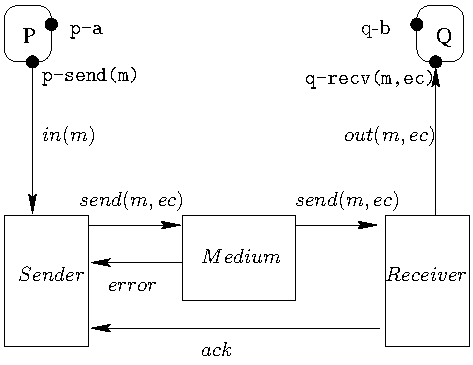
\includegraphics[width=.37\textwidth]{XFIG/SimpleProt-Schema}
   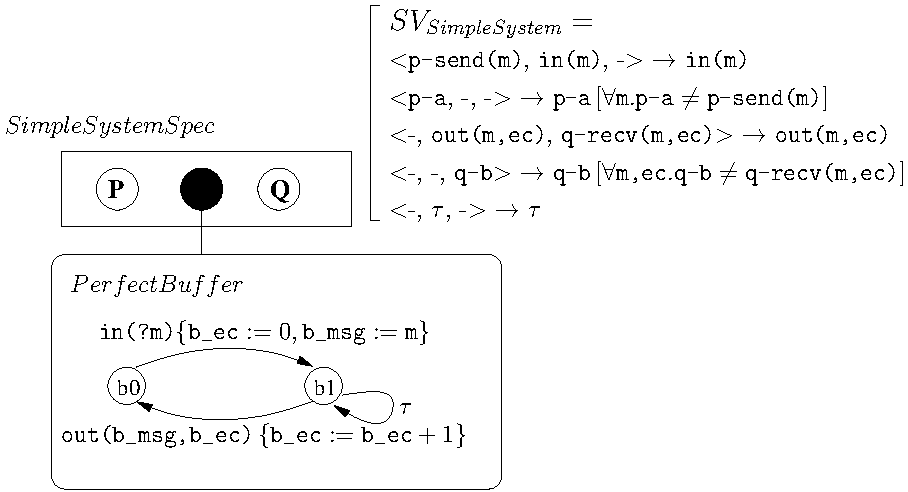
\includegraphics[width=.62\textwidth]{XFIG/SimpleProt2-Spec}
   \caption{pNet structure of the example and specification expressed as a pNet}
   \label{SimpleProt:Spec}

\end{figure}

  
\begin{figure}[t]
  \centerline{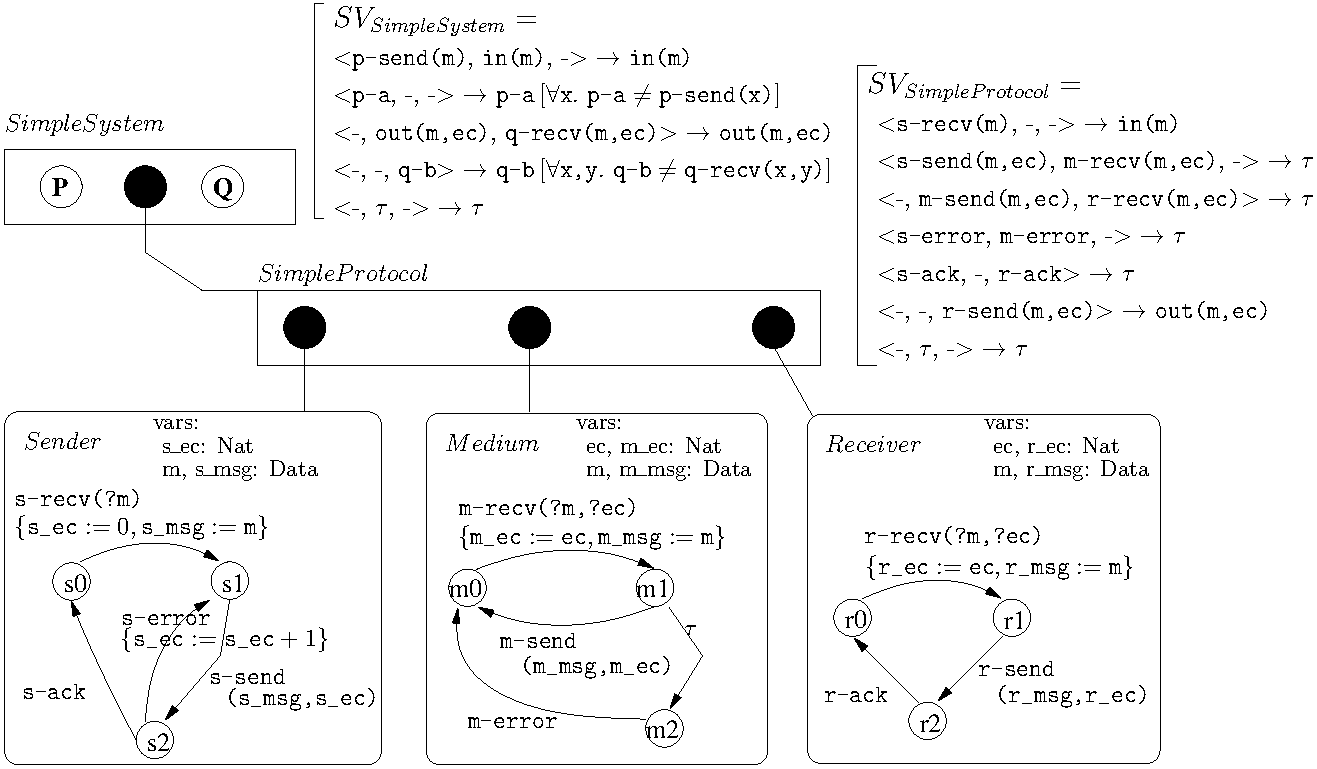
\includegraphics[width=.9\textwidth]{XFIG/SimpleProt2-pNet-tau}}
  \caption{Composed pNet with the Simple Protocol Implementation}  \label{SimpleProt:Impl}
\end{figure}

\section{A model of process composition}\label{sec:OT}


The semantics of open pNets will be defined  as an open automaton. An open
automaton is an automaton where each transition composes transitions of several LTSs with
action of some holes, the transition occurs if some predicates hold, and can involve a 
set of state modifications. This section defines open automata and a bisimulation theory for them.

\subsection{Open Automata}
 Open automata (OA) are not composition structures but they are made of transitions that are dependent of the actions of the holes, and they can reason on variables (potentially with only symbolic values). Formaly, each state of an OA has a set of \emph{state variables}, and all state variable sets are disjoint.
%\TODO{adopt a uniform notation for open transitions, almost each instance has a 
%different 
%notation! I suggest p,l,pr,po using \{\} for p,l,po as they are sets}
\begin{definition}[Open transitions]\label{def:OT}
	\label{def:OpenTransitions}
	An \emph{open transition} (OT) over a
	set $J$ of holes with sorts $\Sort_j^{j\in J}$ and a set of states $\mathcal{S}$ is 
	a structure of the form:	
	\begin{mathpar}
	\openrule
	{	\beta_j^{j\in J'}, \Pred, \Post}
	{s \OTarrow {\alpha}s'}
	\end{mathpar}
	Where $J'\subseteq J$, $s, s'\in\mathcal{S}$ and $\beta_j$
        is a transition of the hole $j$, with $\beta_j\in\Sort_j$. $\alpha$ is an action 
        label denoting the resulting action of this open transition.
        We call \emph{source variables} of an OT the union of all variables
        in the different terms
        $\beta_j$ and $\alpha$, and the state variables of $s$.
        \Pred\ is a predicate over the source variables. \Post\ is a set of 
	assignments that are effective \emph{after the open transition}, they are
        represented as a substitution of the form $({x_k\gets e_k})^{k\in K}$ 
	where $x_k$ are state variables of $s'$, and $e_k$ are expressions
        over the source variables. Open transitions are identified
        modulo logical equivalence on their predicate. 
\end{definition}

It is important to understand the difference between the red dotted rule and a normal 
inference rule. They correspond to two different logical levels.
 The open transition is itself a logical implication, but using a simple logic (this logic includes the boolean expressions $\AlgB$, boolean operators, and term equality). We differentiate classical (black) inference rules that use 
 an expressive logic and are paper rules from open transition rules that use a simpler 
 logic, 
 will be embedded into automata transitions, and could typically be handled in a 
 mechanical way.


An open automaton is then simply an automaton where each transition is an open transition.
\begin{definition}[Open automaton]
	\label{def:open-automaton}
	An \emph{open automaton} is a structure\\ $A =
	<J,\mathcal{S},s_0,\mathcal{T}>$ where:
	\begin{itemize}
		\item[$\bullet$]   $J$ is a  set of indices,
		\item[$\bullet$]   $\mathcal{S}$ is a set of states and $s_0$ an initial state
		  among $\mathcal{S}$,
                  \item[$\bullet$] for each state $s$, $vars(s)=\{v_s\}$ is a set of state variables, and each $v_s$ may have an initial value $init(v_s)$.
		\item[$\bullet$] $\mathcal{T}$ is a set of open transitions and for each
		$t\in \mathcal{T}$ there exist  $J'$ with  $J'
		\subseteq J$, such that $t$ is an open transition over  $J'$
		and  $\mathcal{S}$.
		
	\end{itemize}
		
We take in this article a semantics and logical understanding of these
automata. Open automata are closed by a simple form of refinement that
allows us to refine the predicate, or substitute any free variable by
an expression. More formally, let $\Post$ be any substitution and
$\Pred$ any predicate; suppose $\vars(t)\cap \dom(\Post)=\emptyset$ and
$\vars(t')\cap \dom(\Post)=\emptyset$. Then we have the following
implication: 
	
	 \begin{mathpar}
    \openrule
         {
           \set{\beta}, \Pred\,',\Post\,'}
          {t \OTarrow {\alpha} t'}\in\mathcal{T}
\implies
    \openrule
         {
           \set{\beta}\subst{\Post}, \Pred\,'\subst{\Post}\land\Pred,\Post\shortotimes\Post\,'}
         {t \OTarrow {\alpha\subst{\Post}} {t'}}\in\mathcal{T}
\end{mathpar}
\end{definition}

%\LUDO{I added this paragraph}
Because of the semantic interpretation of open automata, the set of open transition of an open automaton is infinite (for example because every free variable can be renamed). However an open automaton is characterized by a  subset of these open transition which is sufficient to generate, by substitution the other ones. In the following, we will abusively write that we define an ``open automaton'' when we provide only the set of open transitions that is sufficient to generate a proper open automaton by saturating each open transition by all possible substitutions.

Another consequence of the semantics and logical interpretation of the
formulas is that we make no distinction between the equality and the
equivalence on boolean formulas, i.e. equivalence of two predicates
$\Pred$ and $\Pred\,'$ can be denoted $\Pred=\Pred\,'$. 

	
Though the definition is simple, the fact that transitions are complex structures relating events must not be underestimated in order to understand the rest of the article. The first element of theory for open automata, i.e. the definition of a strong bisimulation, is given below.


\subsection{Bisimulation for open Automata}
\label{section:bisimulation}


The equivalence we need is a strong bisimulation between
pNets having exactly the same Holes with the same sorts, but using a
flexible matching 
between open transitions, to accommodate comparisons between pNet
expressions with different architectures.



We define now a bisimulation relation adapted to open automata and their parametric nature. The relation relates states of the open automaton and states equivalence between the open transitions between the states. Its key characteristics are 1) the introduction of predicates in the bisimulation relation: as states may contain variables, relation between states may depend on the value of the variables; 2) the bisimulation property relates elements of the open transitions and take into account predicates over variables, actions of the holes, and state modifications.
 We name it FH-bisimulation,
 as a short cut for the ``Formal Hypotheses'' over the holes behavior manipulated in the
 transitions, but also as a reference to the work of De Simone~\cite{deSimone85},
 that pioneered this idea.

Let $\mathcal{R}=\{(s,t|\Pred_{s,t})\}$ be a relation over the set $\mathcal{S}_1$ and 
$\mathcal{S}_2$ constrained by a predicate
More precisely, for any pair $(s,t)$, there is a 
   single
      $(s,t|\Pred_{s,t})\in\mathcal{R}$  stating that $s$ and $t$ are related 
      if $\Pred_{s,t}$       is 
      \\True, i.e. the states are related when the variables in $s$ and $t$ verify the 
      predicate $\Pred_{s,t}$.
 FH-bisimulation is defined formally: 
 \begin{definition}[Strong FH-bisimulation]\label{def-FH-bisim} ~\\

\noindent
\begin{minipage}{0.69\linewidth} 	Suppose that
   $A_1 = <\!J,\mathcal{S}_1, s_0,
   \mathcal{T}_1\!>$ and $A_2 = <\!J,\mathcal{S}_2,t_0, \mathcal{T}_2\!>$
   are open automata with identical holes of the same sort, with disjoint state variables.  

 Then 
$\mathcal{R}$ is an FH-bisimulation iff for any  states
$s\in\mathcal{S}_1$ and $t\in\mathcal{S}_2$, $(s,t|\Pred_{s,t})\in\mathcal{R}$, we 
have
the following:
\end{minipage}
\hspace{2mm}
\begin{minipage}{0.30\linewidth}
	\includegraphics[width=\linewidth]{XFIG/Bisim}
\end{minipage}




 \begin{itemize}
 \item  For any open transition $OT$ in $\mathcal{T}_1$:
 \begin{mathpar}
     \openrule
         {
           \beta_j^{j\in J'},\Pred_{OT},\Post_{OT}}
         {s \OTarrow {\alpha} s'}

\end{mathpar}
 there exist   open transitions $OT_x^{x\in X} \subseteq \mathcal{T}_2$:
 \begin{mathpar}
%    \left( fresh \ \set{\alpha_i}, \set{b_j}, v_x.\ \
    \openrule
         {
           \beta_{j x}^{j\in J_{x}}, \Pred_{OT_x},\Post_{OT_x}}
         {t \OTarrow {\alpha_x} t_x}
%         \right)
\end{mathpar}
 such that  $\forall x, J'=J_{x}, \exists \Pred_{s',t_x}. (s',t_x|\Pred_{s',t_x})\in 
 \mathcal{R}$; 
 and  \\
 $\Pred_{s,t} \land \Pred_{OT}\implies$\\
%\hspace{1cm}
 $\displaystyle{\bigvee_{x\in X}
   \left( \forall j. \beta_j=\beta_{jx}  \land \Pred_{OT_x}
     \land \alpha\!=\!\alpha_x \land  
     \Pred_{s',t_x}\subst{\Post_{OT}\uplus\Post_{OT_x}}\right)}$
     %     \symb{Subst}(\Pred_{target_x}, \Post_{OT} o \Post_{OT_x})
     %     \right)$.
%\bigskip
%
% $\Pred_{s,t} \land \Pred_{OT}\implies\bigvee_{x\in X} \Pred_x$
%and\\
%%\hspace{1cm}
% $ \forall{x\in X}. \Pred_x \land \Pred_{s,t} \land \Pred_{OT} \Rightarrow
%   \left( \forall j. \beta_j=\beta_{jx}  \land \Pred_{OT_x}
%     \land \alpha\!=\!\alpha_x \land  
%     \Pred_{s',t_x}\subst{\Post_{OT}\uplus\Post_{OT_x}}\right)$
%     %     \symb{Subst}(\Pred_{target_x}, \Post_{OT} o \Post_{OT_x})
%     %     \right)$.



%     \TODO{Eric: j'ai ajoute $\exists$ sur les predicats $\Pred_{s',t_x}$, qui n'etaient pas definis...}
     
 \item  and symmetrically any open transition from $t$ in $\mathcal{T}_2$ can be 
      covered by a set of transitions from $s$ in $\mathcal{T}_1$.
 \end{itemize}

% \TODO{Eric: il reste des petits bugs genre $s^{2'}_x$ plutot que
%   $s^{2}_x$}
 
%Where $\symb{Subst}(\Pred,\Post)$ is the parallel substitution of all
%assigned variables.

% \TODO{do we want formulas for this?}
 \end{definition}
Classically, $\Pred_{s',t_x}\subst{\Post_{OT}\uplus\Post_{OT_x}}$
applies in parallel the  
substitutions $\Post_{OT}$ and $\Post_{OT_x}$ (parallelism is crucial
inside each $\Post$ set but not between  $\Post_{OT}$ and
$\Post_{OT_x}$ that are independent), applying the assignments of the involved rules.
We can prove that such a bisimulation si an equivalence relation:




\begin{theorem}[FH-Bisimulation is an equivalence]\label{thm-equiv} Suppose $\mathcal{R}$ 
is an FH-bisimualtion. Then $\mathcal{R}$ is an equivalence, that is, $\mathcal{R}$ is 
reflexive, symmetric and transitive.
\end{theorem}

The proof of this theorem can be found in~\ref{thm-equiv-proof}. The
only non-trivial part of the proof is the proof of transitivity. It
relies on the following elements. First,  the transitive composition
of two relations with predicate is defined; this is not exactly
standard as it necessitates to define the right predicate for the
transitive composition and producing a single predicate to relate any
two states. Then the fact that one open transition is simulated by a
family of open transitions leads to a doubly indexed family of
simulating open transition; this needs particular care, also because
of the use of renaming (\Post) when proving that the predicates
satisfy the definition (property on $\Pred_{s,t} \land \Pred_{OT}$ in
the definition).  

%\TODO{have a look at the end of the sec}

\medskip



\subsubsection*{Note on finite versus infinite open automata:} as
mentionned in page \pageref{def:open-automaton}, we have defined two flavors of
automata. More precisely, in \cite{hou:hal-02406098}, we formely define
\emph{semantic open automata} (infinite as in Definition \ref{def:open-automaton}),
and \emph{structural open automata} (finite) that can be generated as
the semantics of pNets (see Definition \ref{def:operationalSemantics}), and used in the implementation. Then we define
an alternative version of our bisimulation, called
structural-FH-Bisimulation, based on structural open automata, and
prove that the \emph{semantic} and \emph{structural} FH-Bisimulations coincide.
In the sequel, all mentions of finite automata, and algorithms for
bisimulations, implicitly refer to their \emph{structural} versions.

If we assume that everything is finite (states and transitions in the
open automata, and the predicates in $\mathcal{R}$, then it is easy to
prove that it is decidable whether a relation is a 
FH-bisimulation, provided the logic of the predicates is
decidable (proof in \cite{henrio:Forte2016}). Formally:

\begin{theorem}[Decidability of FH-bisimulation]
Let $A_1$ and $A_2$ be finite open automata
and $\mathcal{R}$ a relation over their states $\mathcal{S}_1$ and
$\mathcal{S}_2$ constrained by a finite set of predicates. Assume that
the predicates inclusion is decidable over  
the action algebra $\mathcal{A}_P$. Then it is decidable whether the relation 
$\mathcal{R}$ is a FH-bisimulation.
  
\end{theorem}



\section{Semantics of Open pNets}
\label{section:op-semantics}

This section defines the semantics of an open pNet as a translation into an open automaton. 
In this translation, the states of the open automata are obtained from
the states of the pLTSs at the leaves of the composition. The
predicates on the transitions are obtained both from the predicates on
the pLTSs transitions and from the synchronisation vectors involved in
the transition. 

The definition of bisimulation for open automata allows us to derive a
bismulation theory for open pNets. As pNets are composition
structures, it then makes sense to prove composition lemmas: we prove
that the composition of strongly bisimilar pNets are themselves
bisimilar. 

\subsection{Deriving an open automaton from an open pNet}
To derive an open automaton from a pNet, we need to describe the set of states of the automaton, and then we will detail the construction rule for transitions of the automaton, this will rely on the derivation of predicate unifying synchronisation vectors and the actions of the pNets involved in a given synchronisation.

%Then the semantics of a pNet is characterized by a set of {\em open
%transitions}, where the hypotheses on process parameters are
%replaced by 1) transitions of the pLTSs at the leaves, and 2) formal
%hypotheses on the transitions of the holes. A {\em predicate} is used
%to relate the parameters and names appearing in the actions of the
%leaves and the holes involved in the rules, but also appearing in  the resulting action.

We define first states of open pNets as tuples of states. We denote them
 as $\triangleleft\ldots\triangleright$ for distinguishing tuple 
states from other tuples.
\begin{definition}[States of open pNets]\label{def-states}
  A state of an open pNet is a tuple (not necessarily finite) of the
  states of its leaves.

  For any pNet \pNet, let $\Leaves(\pNet) = \mylangle S_i,{s_i}_0, \to_i\myrangle^{i \in L}$ be 
  the set of pLTS at its leaves,
  then $States(\pNet) = \{\triangleleft s_i^{i\in L}
  \triangleright| \forall i\in L. s_i \in S_i\}$.
A pLTS being its own single leave:
  $States(\mylangle S,s_0, \to\myrangle) = \{\triangleleft s \triangleright| s \in S\}$.

The initial state is defined as:
$InitState(\pNet) = \triangleleft {{s_i}_0}^{i\in L}  \triangleright$.
\end{definition}



%% \begin{example} \emph{State of a pNet}
%%   The states of pNet \texttt{EnableCompL} are:
%%   $\triangleleft 00 \triangleright, \triangleleft 10 \triangleright, \triangleleft 11 \triangleright$
%% \end{example}

\paragraph{Predicates:}
%Let
%$\mylangle\set{\pNet},\set{\Sort},\set{\symb{SV}}\myrangle$
%be a pNet. 
Consider a synchronisation vector $\SV{{(\alpha'_i)}^{i\in I}, {(\beta'_j)}^{j\in J}} 
{\alpha'} 
{e_b}$. We 
define a
predicate $\Predsv$ relating
the actions of the involved sub-pNets and the resulting actions. This predicate verifies:
\[\begin{array}{l}\Predsv \Big(\SV{{(\alpha'_i)}^{i\in I}, {(\beta'_j)}^{j\in J}} 
{\alpha'} 
{e_b}, \alpha_i^{i\in I}, \beta_j^{j\in J}, \alpha\Big)\Leftrightarrow \\~\qquad\qquad%\bigg(
%
%\exists {(\alpha'_i)}^{i\in I},
%{(\beta'_j)}^{j\in J},v'.\, SV=
%\\~~\land
\forall i\in I.\, \alpha_i=\alpha'_i\land \forall j \in J.\, \beta_j=\beta'_j \land 
\alpha=\alpha' 
\land e_b
\end{array} 
%\bigg)
\]

Somehow, this predicate entails a verification of satisfiability in the sense that if the 
predicate $\Predsv$ is not satisfiable, then the transition associated with the 
synchronisation will not occur in the considered state, or will occur with a \False\ precondition which is equivalent.
If the action families do not match or if there is no valuation of
variables such that the above formula can be ensured the predicate is undefined.

The definition of this predicate is not constructive but it is easy to build the predicate constructively by brute-force unification of the sub-pNets actions with the corresponding vector actions, possibly followed by a simplification step.



%\TODO{Eric: rewrite example with new Protocolkeep only OT1, and adapt comments}
\begin{example}[An open-transition]
  \label{OT:SimpleProt}
At the upper level, the $\symb{SimpleSystem}$ pNet of Figure \ref{SimpleProt:Impl} has 2 holes and $\symb{SimpleProtocol}$ as
a subnet, itself containing 3 pLTSs. One of its possible open transitions
(synchronizing the hole $P$
with the $\symb{Sender}$ within the \emph{SimpleProtocol}) is:

 \smallskip\noindent
 \[  OT_1  = \openrule{
      \{\texttt{P}\mapsto \texttt{p-send(m)}\},  [\texttt{m=m'}],
        \{\texttt{s1\_m}\gets \texttt{m}\}
                      }
    {\ostate{s_0,m_0,r_0} \OTarrow{\underline{\texttt{in(m')}}} \ostate{s_1,m_0,r_0}}
    \]

    \smallskip
    The global states here are triples, build as the product of states of the 3 pLTS (remember the Holes have no state). The assignment
    $Post$ uses the variable $\texttt{m}$ from the action of hole $\texttt{P}$ to set the
    value of the sender state variable named $\texttt{s1\_m}$.
    

 %%  The \emph{SimpleProtocol} pNet of Fig. \ref{SimpleProt:Spec} has 3 controllers and no holes. One of its possible open-transition (the sender sending $(m)$ to the medium) is:

 %% \smallskip\noindent
 %% $  OT_2  = \openrule{
 %%   \emptyset; Pred=[send(SV2\_m)=send(s_1\_m);in(SV2\_m)=in(?m)];  \\ Post=\{m_1\_m:=?m\}
 %%                      }
 %%    {\ostate{s_1,m_0,r_0} \OTarrow{\underline{send(SV2\_m)}} \ostate{s_2,m_1,r_0}}
 %%    $

 %%    That can be simplified to:

 %%    \ERIC{Apres application des substitutions et simplification du predicat:}

 %%     $  OT_2  = \openrule{
 %%      \emptyset; Pred=\True;  \\ Post=\{m_1\_m:=s_1\_m\}
 %%                      }
 %%    {\ostate{s_1,m_0,r_0} \OTarrow{\underline{send(s_1\_m)}} \ostate{s_2,m_1,r_0}}
 %%    $

 %%    \smallskip
 %%    Note that the global states shows how the sender and the
 %%    first medium have evolved during this transition, the sender
 %%    moving from $s_1$ to $s_2$, and the first (forward) medium from
 %%    $m_0$ to $m_1$.
 %%    The predicate $Pred$ involves the state variables $s_1\_m$ and
 %%    $s_1\_sb$ of the sender, while the assignment $Post$ sets the
 %%    state variables of the medium.

    \smallskip

\end{example}

We build the semantics of open pNets as an open automaton over the states  given by 
Definition~\ref{def-states}. The open transitions first
 project the global state into states of the leaves, then apply
pLTS transitions on these states, and compose them with the sort of the holes. %The pNet
%structure does not appear in the open-automaton, only the
%set of Holes and the set of Leaves.
The semantics    instantiates fresh variables using the predicate $\fresh(x)$, additionally, for an action 
$\alpha$, $\fresh(\alpha)$ means all variables in $\alpha$ are fresh.


\begin{definition}[Semantics of open pNets]
	\label{def:operationalSemantics}
	The semantics of a pNet $\pNet$ is an open automaton $A\!= 
	<\!\!Holes(\pNet),States(\pNet),InitState(\pNet),\mathcal{T}\!\!>$ where $\mathcal{T}$   is the smallest set of open transitions such that $\mathcal{T}=\{OT\,|\,\pNet \models OT \}$ and	$\pNet \models OT$	is defined by the following  rules:
%	\begin{itemize}
%		\item $J$ is the set of holes: $Holes(p)= J$. 
		%  \item $\set{L}^L = Leaves(p), \set{H}^J = Holes(p)$
%		\item ${\mathcal{S}} = States(p)$ and $s_0 = InitState(p)$
%		\item $\mathcal{T}$ is the smallest set of open transitions		satisfying the rules below:
%	\end{itemize}
	
	%% \TODO{ We should be careful here: after (re) reading "Huimin
	%% 	Lin, 'Symbolic Transition Systems with Assignements', Concur'96" I
	%% 	think handling assignments is not trivial, even for comparisons of pLTSs. }


	
	The rule for a pLTS  checks that the guard 
	is verified and transforms assignments into post-conditions:		
\begin{mathpar}\inferrule
		{ s \xrightarrow{\langle \alpha,~e_b,~(x_j\!:= {e}_j)^{j\in
					J}\rangle} s'\in \to  }
		{ \mylangle  S,s_0, \to \myrangle
			\models
			\openrule
			{\emptyset ,
			e_b,\left\{x_j\gets e_j\right\}^{j\in J}}
			{\ostate{s} \OTarrow{\alpha} \ostate{s'}}
		}\quad {\TrUn}
\end{mathpar}
%	Note that this note is greatly simplified by the fact that variables are local to 
%	thread; introducing global state variables or accepting loops to the same 
%	state would 
%	require to reason 
%	on the scope of 
%	each variables, and to introduce additional variables to handle the several occurence 
%	of the same pLTS variable in the predicates. Indeed the constraints on pLTS 
%	transitions 
%	ensure that the same variable never appears both on the left and on the right of the 
%	equations of a predicate.
	
	The second rule deals with pNet nodes: for each possible
	synchronisation vector (of index $k$) applicable to the rule subject, the premisses
	include one {\em open transition} for each sub-pNet involved , one possible
	{\em action} for each Hole involved, and the predicate relating these
	with the resulting action of the vector. The sub-pNets involved are split between two 
	sets, $I_2$ for subnets that are pLTSs, and $I_1$ for the others, $J$ is the set of 
	holes involved in the transition\footnote{Formally, if $SV_k \!=\! \SV{({\alpha'})_m^{m 
	\in M}}{\alpha'}{e_b}$ is a synchronisation vector  of \pNet\  then $J=M\cap 
	\Holes(\pNet)$, $I_2=M\cap \Leaves(\pNet)$,  $I_1=M\setminus J \setminus 
	I_2$}.                                                                    
\begin{mathpar}
    \mprset {vskip=.8ex}
\inferrule
    {
\Leaves(\mylangle {\pNet}_m^{m\in I}, \set{\Sort}, \symb{SV}_k^{k\in 
    	K}\myrangle) \!=\! \pLTS_l^{l\in L} \qquad  	
k\!\in\! K \qquad SV_k \!=\! \SV{(\alpha'_m)^{m \in I_1\uplus I_2\uplus J}}{\alpha'}{e_b} 
\\
\\     	
	\forall m\!\!\in\!\! I_1. {\pNet_m 
	\models\openrule
    	{
    	\beta_{j}^{j\in J_m}, \Pred_m, \Post_m}
    	{\ostate{s_{i}^{i \in L_m}} \OTarrow {\alpha_m}
    		\ostate{(s_i^\prime)^{i\in L_m}}} }	
  \qquad
\forall m\!\!\in\!\! I_2.		{ \pNet_m 
    	 \models
    	\openrule
    	{\emptyset, \Pred_m, \Post_m}
    	{\ostate{s_m} \OTarrow {\alpha_m}
    		\ostate{s_m'}} }\\\\
    J' = \biguplus_{m\in I_1}\!\! J_m \uplus J	\\
    	\Pred = \bigwedge_{m\in I_1\uplus I_2}\!\! \Pred_m \land
    	\Predsv(SV_k,\alpha_m^{m\in I_1\uplus I_2},\beta_j^{j\in J},\alpha)\\ 
    	\forall i\in	L\backslash \left(\biguplus_{m\in I_1}\!\! L_m \uplus I_2\right).\,s'_i=s_i \\
    \fresh(\alpha'_m,\alpha',\beta_j^{j\in J},\alpha) 
    }
    {\mylangle {\pNet}_m^{m\in I}, \set{\Sort}, \symb{SV}_k^{k\in K}\myrangle
    	\models
    	{\openrule
    		{
    		\beta_j^{j\in J^\prime}, \Pred,  \biguplus_{m\in I_1\uplus I_2} 
    		\Post_m}
    		{\ostate{s_i^{i\in L}} \OTarrow {\alpha}
    			\ostate{(s_i^\prime)^{i\in L}}}
    	}
    }\quad {\TrDeux}
\end{mathpar}    
	\medskip
%        \TODO{may be explain how $\Pred(SV,a_i^{i\in I_k},b_j^{j\in
%            J_k},v)$ is built ? You mean more than what is written on previous page????}
	%%    \TODO{I have tentatively added the sort constraint on hole actions, that was
	%%not included in the first version... I'm unsure whether this is the best place to
	%%include it, because it may change the decidability conditions on predicates}
\end{definition}
        	A key to understand this rule is that the open transitions are
	expressed in terms of the leaves and holes of the pNet structure,
	i.e. a flatten view of the pNet: e.g. $L$ is the index set of the
	Leaves, $L_m$ the index set of the leaves of one subnet indexed $m$, so all $L_m$
	are disjoint subsets of $L$. Thus the states in the open transitions,
	at each level, are tuples including states of all the
	leaves of the pNet, not only those involved in the chosen
	synchronisation vector.


Note that  the construction is symbolic, and each open-transition deduced expresses a whole family of
behaviours, for any possible values of the variables.
%

In \cite{henrio:Forte2016}, we have shown a detailed example of the construction of a complex open transition, building a deduction tree using rules \TrUn and \TrDeux.

%% \LUDO{Je sais pas de quoi parle le prochain todo :-( l'exemple?}
%% \TODO{Ceci n'est pas nouveau, n'est-ce pas, est-ce utile pour le lecteur ici ? Ou est-ce qu'on bouge tous ces ``details techniques'' dans une annexe ? Si oui, je refais avec un morceau de ABP}
%% \begin{example} \emph{Using the operational rules to compute
%%     open-transitions}
%%   In Fig. \ref{usingrules:OT2} we show the deduction tree used to construct and prove the 
%%   open transition $OT_2$ of \texttt{EnableCompL} (see example page \pageref{OT:ABP-composed}).
%%   The rule uses \TrUn\ for the $\delta$ transition of $C_3$, for the $l$ transition of $C_4$, then combines the result using the $a_4$ vector of the bottom pNet node, and the $\underline{\delta(x)}$ vector of the top node.
  
%% \begin{figure}[h]
%% \begin{mathpar}
%%   \small
%%   \inferrule
%%     {\inferrule
%%         {0 \xrightarrow {\delta}_{C_3} 1}
%%         {C_3
%%           \models
%%             \openrule{
%%               0 \xrightarrow {\delta}_{C_3} 1,\,
%%               \{\xrightarrow{\delta(x_1)}_P\},\,
%%               v_1=\delta(x_1)}
%%                       {\ostate{0}\OTarrow{v_1}\ostate{1}}
%%         }\\
%% %      \sm{fresh}v         \\
%%       \inferrule%*[right={L_1}]
%%         {
%% %          \sm{fresh}{a_Q} \\
%%           \inferrule
%%               {0 \xrightarrow{l}_{C_4} 0}
%%               % {\ostate{0}\xrightarrow{l}\ostate{0}}
%%               {C_4
%%                 \models
%%                 \openrule{
%%                       0 \xrightarrow l_{C_4} 0,\,
%%                       \sm{Pred}_{C_4}}
%%                       {\ostate{0}\OTarrow{l}\ostate{0}}
%%               }
%%         }
%%         {
%%           \textrm{Q>>R}\models
%%               \openrule
%%                   { 0 \xrightarrow {l}_{C_4} 0,\,
%%                     \{\xrightarrow{acc(x_2)}_Q\},\,
%%                     \ v_2=acc(x_2)
%%                   }
%%                   {\ostate{0}\OTarrow{v_2}\ostate{0}}
%%         }   
%%     }
%%     {
%%      \textrm{P>>(Q>>R)}
%%      \models
%%      \openrule
%%          { 0 \xrightarrow{\delta}_{C_3} 1, \\ 0 \xrightarrow{l}_{C_4} 0,\\
%%            \{\xrightarrow{\delta(x)}_P,\,\xrightarrow{acc(x)}_Q\}, \\
%%             a_3=v_1 \wedge v=a_3 \wedge x_1=x_2
%%            }
%%          {\ostate{00} \OTarrow{v} \ostate{10}}
%%       }\vspace{-4ex}
%% \end{mathpar}
%%   \caption{Proof of transition $OT_2$ (with interaction of processes $P$ and $Q$) for 
%%   ``P>>(Q>>R)'' \TODO{Change for the new example or remove?}}
%%   \label{usingrules:OT2}
%% \end{figure}

%% \end{example}




We have shown in \cite{henrio:Forte2016} that an open-pNet
with finite synchronisation sets, finitely many leaves and
holes, and each pLTS at leaves having a finite number of states and
(symbolic) transitions, has a finite automaton. The algorithm for building such an automaton can be found in~\cite{QBMZ-AVOCS18}.

%% \subsection{Post-processing: Elimination of intermediate variables}

%% While building the open transitions, many new variable names are
%% created, as fresh local variables of synchronisation vectors, and
%% fresh result variables of intermediate OTs. While these are required
%% for the semantic construction, they are not significant in the
%% resulting open automaton. In fact they carry information on the
%% internal structure of the pNet system, and this information should
%% \_not\_ be visible when looking at the system as a black box, and in
%% particular when comparing its behaviour with another system, e.g. by
%% bisimulation. 

%% In the resulting predicate the only significant variables are :\\
%% - the input variables of pLTS transitions \TODO{heu, non, meme pas, si
%%   ce sont des comm internes!}\\
%% - the actions of holes\\
%% - the result action at toplevel.

%% So we transform the predicates of the resulting OTs, eliminating all
%% intermediate variables. \TODO{Explain why this should work !! Maybe
%%   need to be more precise on unification in the matching...} 


%\TODO{Eric: full (???) result of the tool execution on the running example on the Simple Prot Spec: Done, on the Counetr version !}

%\begin{figure}[ht]
%   \centerline{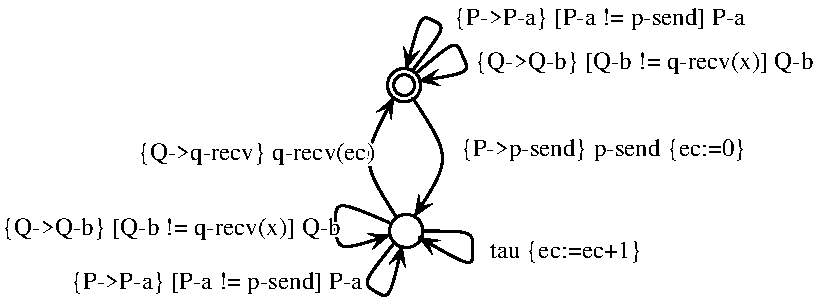
\includegraphics[width=11cm]{ATG/SPSpecOpen}}
%   \caption{Specification OA}
%   \label{SimpleProtCounter:SpecOA}
%\end{figure}



\begin{figure}[ht]
   \centerline{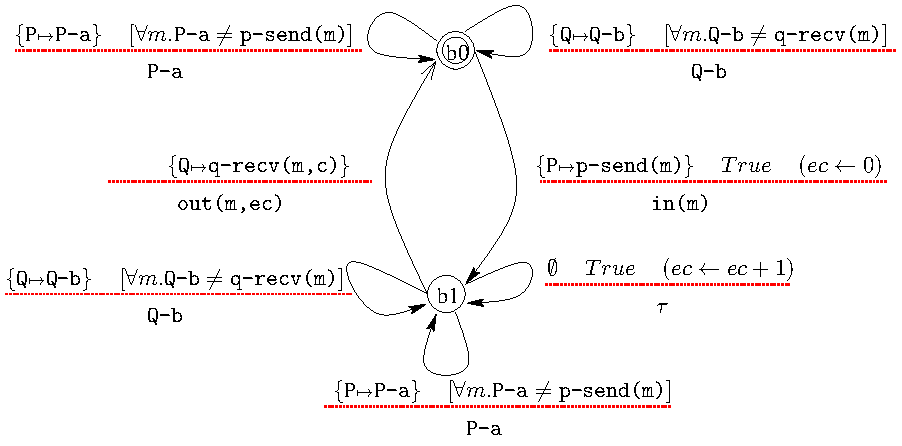
\includegraphics[width=12cm]{XFIG/SPSpecOpen}}
   \caption{Specification OA}
   \label{SimpleProtCounter:SpecOA}
\end{figure}


\paragraph{Example} Figure \ref{SimpleProtCounter:SpecOA} shows the open automaton computed from the Specification pNet given in Figure \ref{SimpleProt:Spec}. 
For later references, we give to the transitions of this (strong)
Specification automaton as $SS_i$ while transitions of the
Implementation automaton will be labelled $SI_i$. In the figure we
have annotated each global state with the set of corresponding state variables.


 \begin{figure}[ht]
  \centerline{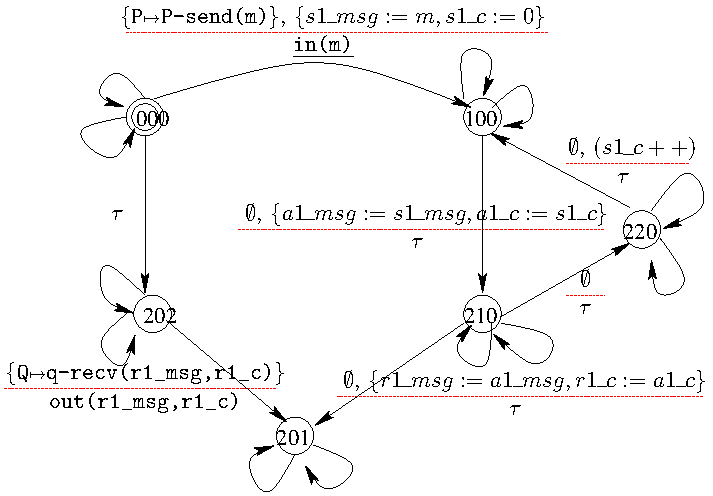
\includegraphics[width=15cm]{XFIG/SPImplOpen}}
  \caption{Open Automaton of the Simple Protocol Implementation}  \label{SimpleProtCounter:ImplOA}
\end{figure}


    Figure \ref{SimpleProtCounter:ImplOA} shows the open automaton of the implementation $SimpleSystem$ (Figure \ref{SimpleProt:Impl}). In this drawing, we have short labels for states, representing $\ostate{s_0,m_0,r_0}$ by \texttt{000}. Note that open transitions are denoted $\texttt{OT}_i$ and tau open transition by  $\texttt{OT}_{\tau}$. The resulting behavior is quite simple:  we have a main loop including receiving a message from $P$ and transmitting the same message to $Q$, with some intermediate $\tau$ actions from the internal communications between the protocol processes. In most of the transitions, you can observe that data is propagated between the successive state variables (holding the message, and the error counter value). On the right of the figure, you have a loop of $\tau$ actions ($\texttt{OT}_4$, $\texttt{OT}_5$ and $\texttt{OT}_6$)  showing the handling of errors and corresponding increments of the error counter.
    
    
  

\subsection{pNet Composition Properties: composition of open transitions}
The semantics of open pNets allows us to prove two crucial properties relating pNet composition with pNet semantics: open transition of a composed pNet can be decomposed into open transitions of its composing sub-pNets, and conversely, from the open transitions of sub-pNets,  an open transition of the composed pNet can be built.

We start with decomposition: from one open transition of $P[Q]_{j_0}$, we exhibit 
corresponding behaviours of $P$ and $Q$, and determine the relation between their 
predicates:
\begin{lemma}[Open transition decomposition\label{lem-decompose}] Consider two pNets $P$ and $Q$ that are not pLTSs\footnote{A similar lemma can be proven for a pLTS $Q$}.
	Let $\Leaves(Q)=p_l^{l\in L_Q}$; suppose:
	\[ P[Q]_{j_0}  
		\models
		{\openrule
			{
				\beta_j^{j\in J}, \Pred,  
				\Post}
			{\ostate{s_i^{i\in L}} \OTarrow {\alpha}
				\ostate{s_i'^{\, i\in L}}}
		}
	\]
		with  $J\cap\Holes(Q)\neq\emptyset$ or $\exists i\in L_Q.\,s_i\neq s'_i$, i.e. $Q$ takes part in the reduction.
		 Then there exist $\alpha_Q$, $\Pred\,'$, $\Pred\,''$, 
		$\Post\,'$, $\Post\,''$ s.t.:\\[-2ex]
		%\[
		\begin{mathpar}
		P\models{\openrule
			{
				\beta_j^{j\in (J\setminus \Holes(Q)) \cup \{j_0\}}, 
				\Pred\,',  
				\Post\,'}
			{\ostate{s_i^{i\in L\setminus L_Q}} \OTarrow {\alpha}
				\ostate{s_i'^{\,i\in L\setminus L_Q}}}
		}%\]
	\vspace{-2.2ex}\\\text{and~~}
		%\[
		Q\models{\openrule
			{
				\beta_j^{j\in J\cap\Holes(Q)}, \Pred\,'',  
				\Post\,''}
			{\ostate{s_i^{i\in L_Q}} \OTarrow {\alpha_Q}
				\ostate{s_i'^{\,i\in L_Q}}}
		}%\]
		\end{mathpar}
		and  $\Pred \iff \Pred\,'
		\land \Pred\,''\land \alpha_Q=\beta_{j_0}$, $\Post=\Post\,'\uplus 
		\Post\,''$ where $\Post\,''$ is the restriction of $\Post$ over variables of 
		$\Leaves(Q)$.
\end{lemma}


Lemma \ref{lem-compose} is combining an open transition of $P$ with
an open transition of $Q$, and building a corresponding transition of
$P[Q]_{j_0}$, assembling their predicates.

\begin{lemma}[Open transition composition]\label{lem-compose} 
	Suppose $j_0\in J$ and:\\[-2ex]
\begin{mathpar}
%\[
P\models{\openrule
	{
		\beta_j^{j\in J}, 
		\Pred,  
		\Post}
	{\ostate{s_i^{i\in L}} \OTarrow {\alpha}
		\ostate{s_i'^{\, i\in L}}}
}%\]
\text{~~and~~}
%\[
Q\models{\openrule
	{
		\beta_j^{j\in J_Q},
		 \Pred\,',  
		\Post\,'}
	{\ostate{s_i^{i\in L_Q}} \OTarrow {\alpha_Q}
		\ostate{s_i'^{\, i\in L_Q}}}
}%\]
\end{mathpar}
Then, we have\\[-2ex]
	\[ P[Q]_{j_0}  
	\models
	{\openrule
		{
			\beta_j^{(j\in J\setminus\{j_0\}) \uplus J_Q}, 
			\Pred\land\Pred\,'\land \alpha_Q=\beta_{j_0},  
			\Post\uplus \Post\,'}
		{\ostate{s_i^{i\in L\uplus L_Q}} \OTarrow {\alpha}
			\ostate{s_i'^{\, i\in L\uplus L_Q}}}
	}
	\]
\end{lemma}

Note that this does not mean that any two pNets can be composed and produce an open 
transition. Indeed, the predicate $\Pred\land\Pred\,'\land \alpha_Q=\beta_{j_0}$ is often not  satisfiable, for example if the action  $\alpha_Q$ cannot be matched with $\beta_{j_0}$.
Note also that $\beta_{j_0}$ is  only used as an intermediate term inside formulas in the composed open transition: it 
does not appear neither as global action nor as an action of a hole.


\subsection{Bisimulation for open pNets -- a Composable Bisimulation Theory}
\label{section:bisimulation-PN}
As  our symbolic operational semantics provides an open automaton, we can apply the notion of
	strong (symbolic) bisimulation on automata to open pNets:
\begin{definition}[FH-bisimulation for open pNets]\label{def:bisim-pnets}
Two pNets are FH-bisimilar if there exist a relation between their associated 
automata that is an FH-bisimulation and their initial states are in the relation (i.e. the predicate associated with the initial states is verifiable).
%\TODO{check}
\end{definition}
%\TODO{Predicate=True me pose un probleme... typiquement, on a besoin d'une ``condition initiale'', pour avoir des pNets data-oriented equivalents a leur version state-oriebted => remove the constraint}

We can now prove that pNet composition  preserves
FH-bisimulation. More precisely, one can define two preservation
properties, namely 1) when one hole of a pNet is filled by two bisimilar other (open) pNets; and 2) when the same hole in two bisimilar pNets are
filled by the same pNet, in other words, composing a pNet with two
bisimilar contexts. The general case will be obtained by
transitivity of the bisimulation relation (Theorem~\ref{thm-equiv}). 

\begin{theorem}[Congruence]\label{thm-congr-eq}
	Consider an open pNet:
	$\pNet = \mylangle \pNet_i^{i\in I}, \Sort_j^{j\in J}, 
	\set{\symb{SV}}\myrangle$.
	Let $j_0\in J$ be a hole. Let $\pNetQ$ and $\pNetQ'$ be two FH-bisimilar pNets such that 
	$\Sortop(\pNetQ)=\Sortop(\pNetQ')=\Sort_{j_0}$\footnote{Note that $\Sortop(\pNetQ)=\Sortop(\pNetQ')$ is 
	ensured by 
	strong bisimilarity.}. Then 
	$\pNet[\pNetQ]_{j_0}$ and 
	$\pNet[\pNetQ']_{j_0}$ are FH-bisimilar.
\end{theorem}
 
 
\begin{theorem}[Context equivalence]\label{thm-ctxt-eq}
	Consider two FH-bisimilar open pNets:
	$\pNet = \mylangle \pNet_i^{i\in I}, \Sort_j^{j\in J}, 
	\set{\symb{SV}}\myrangle$ and 	$\pNet' = \mylangle {\pNet'}_i^{i\in I}, 
	\Sort_j^{j\in 
	J}, 	\set{\symb{SV'}}\myrangle$ 
	(recall they must have the same holes to be bisimilar).
	Let $j_0\in J$ be a hole, and $Q$ be a pNet such that $\Sortop(Q)=\Sort_{j_0}$. Then 
	$\pNet[Q]_{j_0}$ and 
	$\pNet'[Q]_{j_0}$ are FH-bisimilar.
\end{theorem}

Finally, the previous theorems can be composed to state a general theorem about 
composability and FH-bisimilarity.
\begin{theorem}[Composability] \label{thm-composability}
	Consider two FH-bisimilar pNets with an arbitrary number of holes, when replacing, 
	inside those two original pNets, a subset of the holes by FH-bisimilar pNets, we 
	obtain two FH-bisimilar pNets.
\end{theorem}
This theorem is quite powerful. It somehow implies that the theory of open pNets is convenient to study properties of process composition. Open pNets can indeed be used to study process operators and process algebras, as shown in~\cite{henrio:Forte2016}, or to study interaction protocols~\cite{BHHM:FACS11}.

\section{Weak bisimulation}\label{sec:weak}

Weak symbolic bisimulation was introduced to relate transition systems
that have indistinguishable behaviour, with respect to some definition
of \emph{internal actions} that are considered local to some
subsystem, and consequently cannot be observed, nor used for
synchronisation with their context.
The notions of non-observable action varies in different contexts,
e.g. $tau$ in CCS, and $i$ in Lotos, we could define classically a set of
\emph{internal/non-observable actions} depending on a specific action
algebra. In this paper, to simplify the notations, we will simply use $\tau$ as the single non-observable action; the generalisation of our results to a set of non-observable actions is trivial. 
Naturally, a non-observable action cannot be synchronised with
actions of other systems in its environment. 
We show here that under such assumption of non-observability of $\tau$ actions, see Definition~\ref{def:Non-ObsTau}, we can define a weak bisimulation relation that is compositional, in the sense of open pNet composition. In this section we will first define a notion of weak open transition similar to open transition. In fact a weak open transition is made of several open transitions labelled as non-observable transitions, plus potentially one observable open transition. This allows us to define weak open automata, and a weak bisimulation relation based on these weak open automata. Finally, we apply this weak bisimulation to open pNets, obtain a weak bisimilarity relationship for open pNets, and prove that this relation has compositional properties.

%% \TODO{we should understand if it make sense to distinguish invisible
%%   from synchronised actions: in the Forte paper we wrote ``using  as 
%% \emph{invisible actions} a subset of the
%% \emph{synchronised actions} defined in Section~\ref{section:pnets}''}.

%% Proving bisimulation properties on our hierarchical broadcast example
%% would take too much space for this paper. Moreover, interesting
%% properties of the HB example would rather be adequate for weak
%% bisimulation, and its large state-space would require some
%% tool-assistance, both for the generation of the open-automata and for
%% their comparison.

\subsection{Preliminary definitions and notations}


We first specify in terms of open transition, what it means for an action to be non-observable. Namely, we constraint ourselves to system where the emission of a $\tau$ action by a sub-pNet cannot be observed by the surrounding pNets. In other words, a pNet cannot change its state, or emit a specific observable action when one of its holes emits a $\tau$ action.

More precisely, we state that $\tau$ is not observable if the automaton always allows any $\tau$ transition from holes, and additionally the global transition resulting from a $\tau$ action of a hole is a $\tau$ transition not changing the pNet's state.
We define $\Id(s)$ as the identity function on variables of state s.
\begin{definition}[Non-observability of $\tau$ actions]\label{def:Non-ObsTau}
An open automaton $A = <J,\mathcal{S},s_0,\mathcal{T}>$ \emph{cannot observe $\tau$ actions} if and only if for all $j$ in $J$ and $s$ in $\mathcal{S}$ we have:
\begin{enumerate}
\item
\[ \openrule
         {
           (j\mapsto\tau),\True,\Id(s)}
         {s \OTarrow {\tau} s}
         \in \mathcal{T}
\]
and 
\item for all $\beta_j$, $J$,  $\alpha$,  $s$, $s'$, $\Pred$, $\Post$  such that
\[ \openrule
         {
           \beta_j^{j\in J},\Pred,\Post}
         {s \OTarrow {\alpha} s'}
         \in \mathcal{T} \] If there exists $j$ such that $\beta_j=\tau$ then we have: \[ \alpha=\tau\land s=s'\land \Pred=\True\land\Post=\Id(s) \land J=\{j\}
\]
\end{enumerate}
\end{definition}
The first statement of the definition states that the open automaton must allow a hole to do a silent action at any time, and must not observe it, i.e. cannot change its internal state because a hole did a $\tau$ transition. The second statement ensures that there cannot be in the open automaton other transitions that would be able to observe a $\tau$ action from a hole. The condition $J=\{j\}$ is a bit restrictive, it could safely be replaced by $\forall j\in J.\, \beta_j=\tau$, allowing the other holes to perform $\tau$ transitions too (because these $\tau$ actions cannot be observed).


By definition, one weak open transition contains  several open transitions, where  each open transition can require an observable action from a given hole, the same hole might have to emit several observable actions for a single weak open transition to occur. 
Consequently, for a weak open transition to trigger, a sequence of actions from a given hole may be required.

\TODO{Check, nouvelle formulation, Eric}
\LUDO{checked, slight changes}
Thus, we let $\gamma$ range over sequences of action terms and use $\dotcup$ as the concatenation operator that appends sequences of action terms: given two sequences of action terms  $\gamma\dotcup\gamma '$ concatenates the two sequences. The operation is lifted to indexed sets of sequences:  $\set {\gamma_1}\dotcup \set {\gamma_2}$ is an indexed set such that, at each index $i$, $\set {\gamma_1}\dotcup \set {\gamma_2}$ concatenates the sequences of actions at index $i$ of $\set{\gamma_1}$ and the one at index $i$ of $\set {\gamma_2}$\footnote{One of the two sequences is empty when $i\not \in \dom(\set{\gamma_1})$ or $i\not \in \dom(\set{\gamma_2})$ .}. $[a]$ denotes a sequence with a single element.

As required actions are now sequences of observable actions, we need an operator to build them from set of actions that occur in open transitions, i.e. an operator that takes a set of actions performed by one hole and produces a sequence of observable actions.
Thus we define $\vis{\set\beta}$ as the mapping $\set\beta$  with only observable actions of the holes in $I$, but where each element is either empty or a list of length 1:
 \[\vis{\beta_i^{i\in I}} = [\beta_i]^{i\in I'}\text{ where }I'=\left\{i| i\in I \land \beta_i\neq \tau\right\}\]

As an example the $\vis{\set\beta}$ built from the transition $OT_1$ in page \pageref{OT:SimpleProt} is $\texttt{P}\mapsto [\texttt{p-send(m)}]$. Remark that in our simple example no $\tau$ transition involves any visible action from a hole, so we have no $\beta$ sequences of length longer than 1 in the weak automaton.

\subsection{Weak open transition definition}

Because of the non-observability property (Definition~\ref{def:Non-ObsTau}), it is possible to add any number of $\tau$ transitions of the holes before or after any open transition freely. This property justifies the fact that we can abstract away $\tau$ transitions from holes in the definition of a weak open transition.



%
%Classically, we start by defining a derived transition relation based
%on sequences of invisible actions.

\def\InvAct{\mathcal{Inv}}
%
%\RAB{We let $\gamma$ range over words (of action terms) and use $\dotcup$ as the union that appends words.}

\begin{definition}[Weak open transition]\label{def:weakOT}
A weak open transition over a
	set $J$ of holes with sorts $\Sort_j^{j\in J}$ and a set of states $\mathcal{S}$ is 
	a structure of the form:	
\begin{mathpar}
 \openrule
         {
           \gamma_j^{j\in J'},\Pred,\Post}
         {s \OTWeakarrow {\alpha} s'}
 \end{mathpar}
	Where $J'\subseteq J$, $s, s'\in\mathcal{S}$ and $\gamma_j$
        is a list of transitions of the hole $j$, with each element of the list in $\Sort_j$. $\alpha$ is an action 
        label denoting the resulting action
        of this open transition. \Pred\ and \Post\ are defined similarly to Definition~\ref{def:OT}. We use $\WT$ to range over sets of weak open transitions.

A weak open automaton $<J,\mathcal{S},s_0,\WT>$ is similar to an open automaton  except that $\WT$ is a set of weak open transitions over $J$ and $\mathcal{S}$.
\end{definition}

A weak open transition labelled $\alpha$ can be seen as a sequence of open transitions that are all labelled $\tau$ except one that is labelled $\alpha$; however conditions on predicates, effects, and states must be verified for this sequence to be enactable.


We are now able to build a weak open automaton from an open automaton. This is done in a way that resembles the process of $\tau$ saturation: we add  $\tau$ open transitions before or after another (observable or not) open transition.
\begin{definition}[Building a weak open automaton]\label{def:buildweakOT}
  Let $A = <J,\mathcal{S},s_0,\mathcal{T}>$ be an open automaton. 
The weak open automaton \emph{derived} from $A$ is an open automaton  $<J,\mathcal{S},s_0,\WT>$ where $\WT$ is derived from $\mathcal{T}$ as follows: 
%\noindent{\bf Invisible $\tau$ transitions:}
\begin{mathpar}
 \openrule
         {
           \emptyset,\symb{True},\Id(s)}
         {s \OTWeakarrow {\tau} s} \in \WT  \qquad \WTUn
 \end{mathpar}
and
\begin{mathpar}
  \mprset {vskip=.5ex}
\inferrule{
 \openrule
         {
           \set{\beta},\Pred,\Post}
         {s \OTarrow {\alpha} s'} \in \mathcal{T}
} 
{ \openrule
         {
           \vis{\set{\beta}}\!,\Pred,\Post
				 } {s \OTWeakarrow {\alpha} s'} \in \WT
}\qquad \WTDeux
%\inferrule{
% \openrule
%         {
%           \set{\beta},\Pred,\Post}
%         {s \OTarrow {\tau} s'} \in \mathcal{T}
%\\
% \openrule
%         {
%           \set{\gamma},\Pred\,',({x_k\gets e_k})^{k\in K}   }
%         {s' \OTWeakarrow {\tau} s''} \in \WT
%}
%{ \openrule
%         {
%           \vis{\set{\beta}}\dotcup\set{\gamma},\Pred\land\Pred\,'\subst{\Post\,},
%				({x_k\gets (e_k\subst{\Post\,})})^{k\in K} } 
%         {s \OTWeakarrow {\tau} s''} \in \WT
%}
 \end{mathpar}
 and
%\noindent{\bf Other transitions:}
\begin{mathpar}
  \mprset {vskip=.5ex}
\inferrule {\openrule
         {
           \set{\gamma_1},\Pred_1,\Post_1   }
         {s \OTWeakarrow {\tau} s_1} \in \WT
\qquad
\openrule
         {
           \set{\gamma_2},\Pred_2,\Post_2  }
         {s_1 \OTWeakarrow {\alpha} s_2} \in \WT
\qquad
\openrule
         {
           \set{\gamma_3},\Pred_3,\Post_3  }
         {s_2 \OTWeakarrow {\tau} s'} \in\WT
\\
\Pred=\Pred_1\land\Pred_2\subst{\Post_1}\land \Pred_3\subst{\Post_2\shortotimes\Post_1}
\\
\set{\gamma}=\set{\gamma_1}\dotcup \set{\gamma_2}\subst{\Post_1}\dotcup\set{\gamma_3}\subst{\Post_2\shortotimes \Post_1}\\
\alpha'=\alpha\subst{\Post_1}
}
{
\openrule
         {\set{\gamma}
           ,
		\Pred,
				\Post_3\shortotimes\Post_2\shortotimes\Post_1} 
         {s \OTWeakarrow {\alpha'} s'} \in\WT
} \WTTrois
\end{mathpar}
 
\end{definition}
Rule $\WTUn$ states that it is always possible to do a null $\tau$ transition, where the state is unchanged and the holes perform no action. Rule~$\WTDeux$ states that each open transition can be considered as a weak open transition. The last rule is the most interesting:  Rule~$\WTTrois$ allows any number of $\tau$ transitions before or after a weak open transition. This rules carefully composes predicates, effects, and actions of the holes, indeed in the rule, predicate $\Pred_2$ manipulates variables of $s_1$ that result from the first weak open transition. Their value thus depend of the initial state but also of the effect (as a substitution $\Post_1$) of the first weak open transition. In the same manner, $\Pred_3$ must be applied the joint substitution $\Post_2\bigotimes\Post_1$. Similarly, effects on variables must be applied to obtain the global effect of the composed weak open transition, it must also be applied to observable actions of the holes, and to the global action of the weak open transition.

%% \begin{figure}[ht]
%%    \centerline{\includegraphics[width=12cm]{ATG/WOT1}}
%%   \caption{Construction of the Weak Open transition WOT1}
%%    \label{WOT1}
%% \end{figure}

%% \begin{figure}[ht]
%%    \centerline{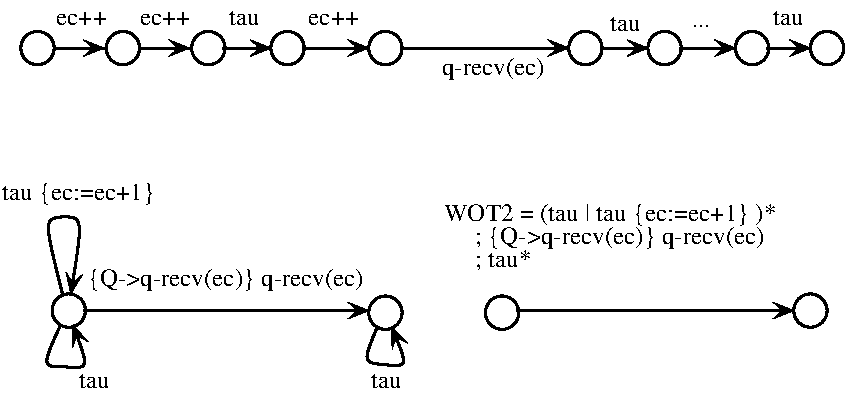
\includegraphics[width=11cm]{ATG/WOT2}}
%%   \caption{Construction of WOT2}
%%    \label{WOT2}
%% \end{figure}

\begin{figure}[ht]
   \centerline{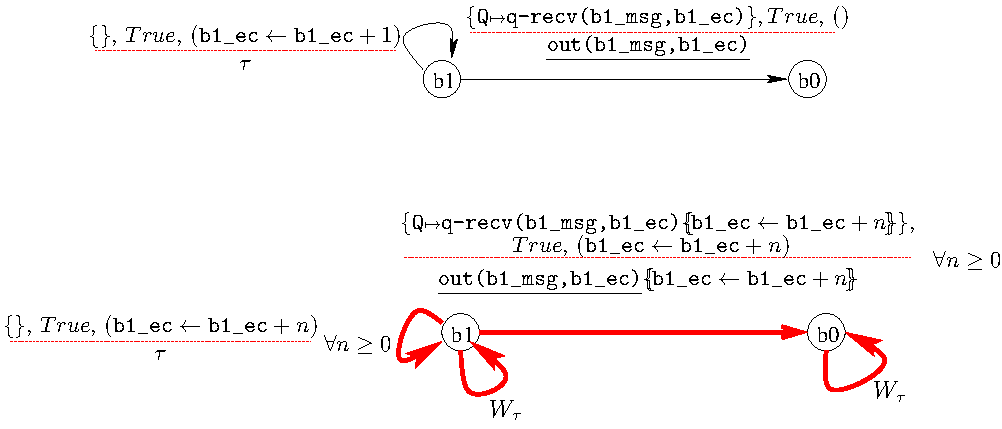
\includegraphics[width=10cm]{XFIG/WOT2-result}}
  \caption{Construction of an example of weak open transition}
   \label{WOT2}
\end{figure}

\begin{example}
  Figure \ref{WOT2} shows the construction of one of the weak transitions of the Specification OA. On the top we show the subset of the original open automaton (from Figure \ref{SimpleProtCounter:SpecOA}) considered here, and at the bottom the generated weak transition.  For reasons of readability, we abbreviate the weak open transitions encoded by $\openrule   {\{\}, True,	() } {s \OTWeakarrow \tau s'}$  as $W_\tau$. The weak open transition shown here is the transition delivering the result of the algorithm to hole $Q$ by applying rules: \WTUn,\WTDeux, and \WTTrois. First rule \WTUn~ adds an $WT_\tau$ loop on each state. Rule \WTDeux~ transforms each 3 OTs into WOTs.   Then consider application of Rule \WTTrois~ on a sequence 3  WOTs.   $\openrule
         {\{\}, True,
			(\texttt{ec}\gets \texttt{ec}+1) }
         {b1 \OTWeakarrow \tau b1}$; $\openrule
         {\{\}, True,
			(\texttt{ec}\gets \texttt{ec}+1) }
         {b1 \OTWeakarrow \tau b1}$;  $\openrule
         {\{\}, True,
			() }
         {b1 \OTWeakarrow \tau b1}$. Then Rule \WTTrois~ produces  $\openrule
         {\{\}, True,
			(\texttt{ec}\gets \texttt{ec}+2) }
         {b1 \OTWeakarrow \tau b1}$. We can  can iterate this construction an arbitrary number of times, getting for any natural number $n$ the weak open transition:
  $\openrule
         {\emptyset, True,
			(\texttt{ec}\gets \texttt{ec}+n) }
         {\text{b}1 \OTWeakarrow \tau b1} \forall n \geq 0$.  Finally,  applying again \WTTrois, and using the central open transition having \texttt{\underline{out(m,ec)}}  as $\alpha$, we get the resulting weak open transition between b1 and b0 (as shown in Figure \ref{WOT2}).
 %     $\openrule
 %        {\{\texttt{Q}\mapsto\texttt{q-revc(ec)}\subst{ec\gets ec+n}\}, True,
%			(\texttt{ec}\gets \texttt{ec}+n) }
 %        {b1 \OTWeakarrow {\underline{\texttt{out(m,ec)}}\subst{ec\gets ec+n}} b0} \forall n \geq 0$. 
\end{example}


  \begin{example}
    Figures \ref{SimpleProtCounter:WeakSpecOA} and \ref{SimpleProtCounter:ImplWOA} respectively show the weak automata of the simple protocol specification and implementation. We encode weak open transitions  by $WS$ on the specification model and by $WI$ on the implementation model.
    
    \TODO{comment...}

    For readability, we did not include the full details of the Implementation weak open transitions in Figure \ref{SimpleProtCounter:ImplWOA}, they will appear below.
First, we point out that the weak OT loops ($WI_1$,$WI_2$ and $W_\tau$) on state ${000}$ are also present in all other states, we did not repeat them. Then many WOTs are similar, and numbered accordingly as 3, 3', 3'', and 8, 8', 8'',8''' respectively: they only differ by the name of the state variables in their respective source or target states.
\end{example}

  

%\begin{figure}[h]
%   \centerline{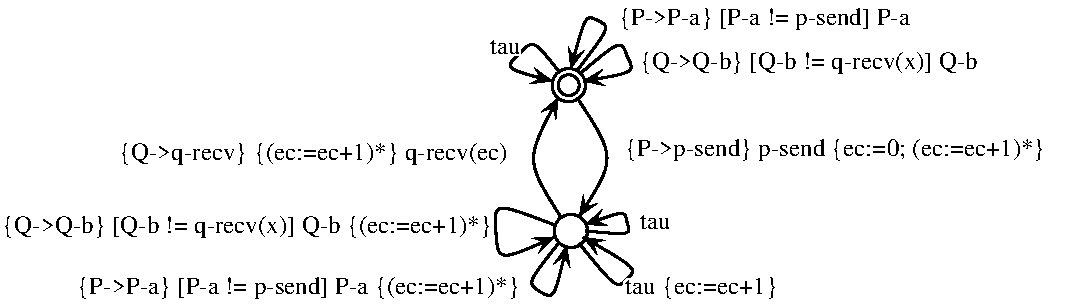
\includegraphics[width=13cm]{ATG/SPSpecWeakOpen}}
%  \caption{Weak Open Automaton of the Specification \TODO{out of date}}
%   \label{SimpleProtCounter:WeakSpecOA}
%\end{figure}


\begin{figure}[h]
   \centerline{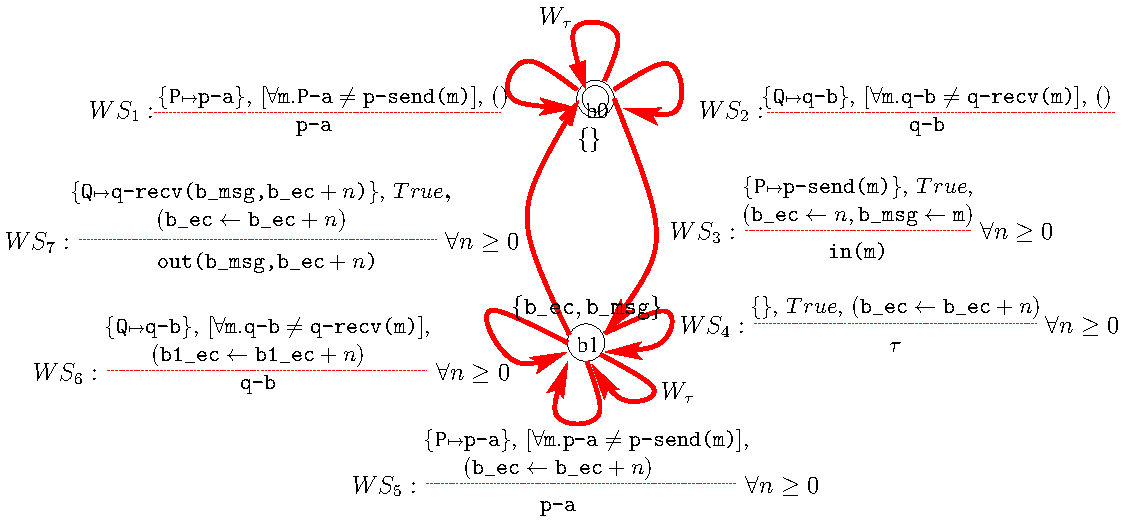
\includegraphics[width=15cm]{XFIG/SPSpecWeakOpen}}
  \caption{Weak Open Automaton of the Specification}
   \label{SimpleProtCounter:WeakSpecOA}
\end{figure}

\begin{figure}[h]
   \centerline{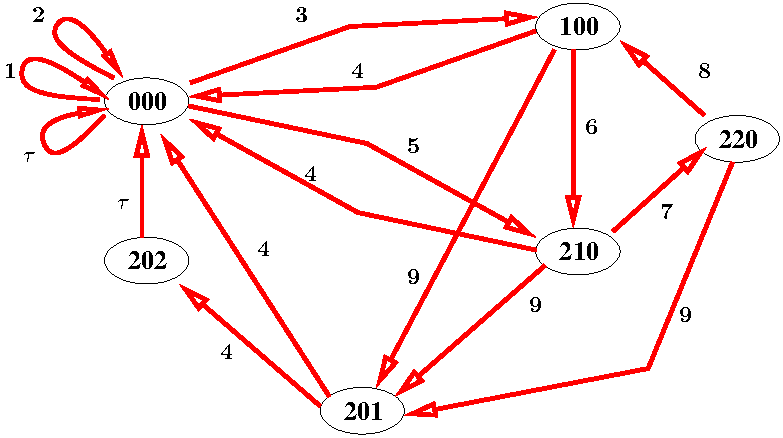
\includegraphics[width=11cm]{XFIG/SimpleProtImpl-WOA}}
  \caption{Weak Open Automaton of the implementation}
   \label{SimpleProtCounter:ImplWOA}
\end{figure}


Now let us give some details about the construction of the weak automaton of the implementation pNet, obtained by application of the weak rules as explained above. We concentrate on transitions $WT_3$ and $WT_4$. Let us denote as $post_n$ the effect (= substitution) of the strong open transitions $OT_n$ from Figure \ref{SimpleProtCounter:ImplOA}:
\smallskip

$post_3 = (\texttt{s1\_ec}\gets 0, \texttt{s1\_m}\gets \texttt{m})$

$post_4 = (\texttt{m1\_msg}\gets \texttt{s1\_msg}, \texttt{m1\_ec}\gets \texttt{s1\_ec}, \texttt{s2\_ec}\gets \texttt{s1\_ec})$

$post_5 = ()$

$post_6 = (\texttt{s1\_ec}\gets \texttt{s2\_ec+1})$

\medskip

Then the effect of one single $100 \xrightarrow{OT_4} 210 \xrightarrow{OT_5} 220 \xrightarrow{OT_6} 100$ loop is:
\smallskip

$Post_{456} = post_6 \shortotimes\ post_5 \shortotimes\ post_4
= (\texttt{s1\_ec}\gets \texttt{s1\_ec}+1)$.
\medskip

So if we denote ${Post_{456}}^*$ any iteration of this loop, we get ${Post_{456}}^* = (\texttt{s1\_ec}\gets \texttt{s1\_ec}+n)$ for any $n\ge 0$, and the Post of the weak OT $WI_{3}$ is $ {Post_{456}}^*\shortotimes\ post_3 = (\texttt{s1\_msg}\gets m, \texttt{s1\_ec}\gets n), \forall n\ge 0$ and $Post(WI_{3'})$ is $ post_4\shortotimes {Post_{456}}^*\shortotimes\ post_3 = (\texttt{m1\_msg}\gets m, \texttt{m1\_ec}\gets n), \forall n\ge 0$.
\medskip

We can now show some of the weak OTs of Figure \ref{SimpleProtCounter:ImplOA} (the full table is included in Appendix \ref{Appendix:FullExample}) :
\smallskip

$ WI_1 = \openrule
{\{\texttt{P}\mapsto \texttt{p-a}\}, [\forall \texttt{m}. \texttt{p-a} \neq \texttt{p-send(m)} ], ()}
{000 \OTWeakarrow {\tau} 000}$

$ WI_3(n) = \openrule
  {\{\texttt{P}\mapsto \texttt{p-send(m)}\}, True,
    (\texttt{s1\_msg}\gets \texttt{m}, \texttt{s1\_ec}\gets n)}
  {000 \OTWeakarrow {\underline{\texttt{in(m)}}} 100}
  \ \forall n\ge 0$

  $ WI_4(n) = \openrule
         {\{\}, True, (\texttt{m1\_msg}\gets \texttt{s1\_msg}, \texttt{m1\_ec}\gets \texttt{s1\_ec}+n, \texttt{s2\_ec}\gets \texttt{s1\_ec}+n)}
         {100 \OTWeakarrow {\tau} 210}
         \ \forall n\ge 0$

$Post_{8'''}= post_{8}\shortotimes\ post_{7}\shortotimes\ post_{4}\shortotimes\ Post_{456}^*\shortotimes\ post_{6} = (\texttt{r1\_msg}\gets \texttt{s1\_msg}, \texttt{r1\_ec}\gets \texttt{s2\_msg}+1+n), \forall n\ge 0$
         
$ WI_{8'''}(n) = \openrule
         {\{\texttt{Q}\mapsto \texttt{q-recv(s1\_msg,s2\_ec}+n)\}, True, ()}
         {210 \OTWeakarrow {\underline{\texttt{out(s1\_msg,s2\_ec+n)}}} 202}
         \ \forall n\ge 1$

\subsection{Composition properties: composition of weak open transitions}
We now have two different semantics for open pNets: a strong semantics, defined  as an open automaton, and as a weak semantics, defined as a weak open automaton. Like the open automaton, the weak open automaton features valuable composition properties. We can exhibit  a composition property and a decomposition property that relate open pNet composition with their semantics, defined as weak open automata. These are however technically more complex than the ones for open automata because each hole performs a set of actions, and thus a composed transition is the composition of one transition of the top-level pNet and a sequence of transitions of the sub-pNet that fills its hole. They can be found as Lemmas~\ref{lem-decomposeWOT}, Lemma~\ref{lem-Weakcompose1}, and Lemma~\ref{lem-Weakcompose} in~\ref{sec:app-composition}.



\subsection{Weak FH-bisimulation}
For defining a bisimulation relation between weak open automata, two options are possible. Either we define a simulation similar to the strong simulation but based on open automata, this would look like the FH-simulation but would need to be adapted to weak open transitions. Or we define directly and classically a weak FH-simulation as a relation between two open automata, relating the open transition of one open automaton with the transition of the weak open automaton derived from the second one. 

The definition below specifies how a set of weak open transitions can simulate an open transition, and under which condition; this is used to relate, by weak FH-bisimulation, two open automata by reasoning on the weak open automata that can be derived from the strong ones.
This is defined formally as follows.

\begin{definition}[Weak FH-bisimulation]\label{def-Weak-bisim} 

\noindent
Let $A_1 = <J,\mathcal{S}_1, s_0,
    \mathcal{T}_1>$ and $A_2 = <J,\mathcal{S}_2,t_0,  \mathcal{T}_2>$ be open automata with disjoint state variables.
Let $<J,\mathcal{S}_1, s_0,
    \WT_1>$ and $<J,\mathcal{S}_2,t_0,  \WT_2>$ be the
weak open automata derived from $A_1$ and $A_2$ respectively.
Let $\mathcal{R}$ a relation over
$\mathcal{S}_1$ and $\mathcal{S}_2$, as in Definition~\ref{def-FH-bisim}.

Then 
   $\mathcal{R}$ is a weak FH-bisimulation iff for any  states
$s\in\mathcal{S}_1$ and
$t\in\mathcal{S}_2$ such that $(s,t|\Pred)\in\mathcal{R}$, we 
   have the following:



 \begin{itemize}
 \item  For any open transition $OT$ in $\mathcal{T}_1$:
 \begin{mathpar}
     \openrule
         {
           \beta_j^{j\in J'},\Pred_{OT},\Post_{OT}}
         {s \OTarrow {\alpha} s'}

\end{mathpar}
 there exist weak open transitions $\symb{WOT}_x^{x\in X} \subseteq \WT_2$:
 \begin{mathpar}
    \openrule
         {
           \gamma_{j x}^{j\in J_{x}}, \Pred_{OT_x},\Post_{OT_x}}
         {t \OTWeakarrow {\alpha_x} t_x}
\end{mathpar}
 such that  $\forall x, \{j\in J'|\beta_j\neq\tau\}=J_{x}, (s',t_x|\Pred_{s',t_x})\in \mathcal{R}$; 
 and  \\
 $\Pred \land \Pred_{OT}\\
\hspace{1cm} \implies\!\!\! \displaystyle{\bigvee_{x\in X}\!
   \left( \forall j\in J_x. \vis{\beta_j}\!=\!\gamma_{jx}\! \land\! \Pred_{OT_x}
     \!\land\! \alpha\!=\!\alpha_x\! \land\!  
     \Pred_{s',t_x}\subst{\Post_{OT}\uplus\Post_{OT_x}}\right)}$
    
 \item  and symmetrically any open transition from $t$ in $\mathcal{T}_2$ can be 
      covered by a set of weak transitions from $s$ in $\WT_1$.
 \end{itemize}

Two pNets are weak FH-bisimilar if there exists a relation between their associated 
automata that is a Weak FH-bisimulation and their initial states are in the relation, i.e. 
the predicate associated to the relation between the initial states is \True.
 \end{definition}

Compared to strong bisimulation, except the obvious use of weak open transitions to simulate an open transition, the condition on predicate is slightly changed concerning actions of the holes. Indeed only the visible actions of the holes must be compared and they form a list of actions, but of length at most one.

In practice, we are dealing with finite representations of the (infinite) open automata. In \cite{hou:hal-02406098}, we defined a slightly modified definition of the ``coverage'' proof obligation, in the case of strong FH-Bisimulation. This modification is required to manage in a finite way all possible instantiations of an OT. In the case of weak FH-Bisimulation, the proof obligation from definition \ref{def-Weak-bisim} becomes:
      
 $\forall fv_{OT}. \{ \Pred \land \Pred_{OT}\\
\hspace{1cm} \implies\!\!\! \displaystyle{\bigvee_{x\in X}\!
  \left[\exists fv_{OT_x}.\\
    \left( \forall j\in J_x. \vis{\beta_j}\!=\!\gamma_{jx}\! \land\! \Pred_{OT_x}
     \!\land\! \alpha\!=\!\alpha_x\! \land\!  
     \Pred_{s',t_x}\subst{\Post_{OT}\uplus\Post_{OT_x}}\right)\right]\}}$

In which $fv_{OT}$ denotes the set of free variables of all expressions in $OT$.

\medskip
Our first important result is that Weak FH-bisimilarity is an equivalence in the same way as strong FH-bisimilarity:


\begin{theorem}[Weak FH-Bisimulation is an equivalence]\label{thm-weak-equiv} Suppose $\mathcal{R}$ 
is a weak FH-bisimulation. Then $\mathcal{R}$ is an equivalence, that is, $\mathcal{R}$ is 
reflexive, symmetric and transitive.
\end{theorem}
The proof  is detailed in Appendix \ref{app-WFH-equiv}, it follows a similar pattern as the proof that strong FH-bisimulation is an equivalence, but technical details are different, and in practice we rely on a different (but proven equivalent) definition of weak FH-bisimilarity; this equivalent version simulates a \emph{weak} open transition with a set of weak open transition. The careful use of the best definition of weak FH-bisimilarity makes the proof similar to the strong FH-bisimulation case.



\subsection{Weak bisimulation for open pNets}

Before defining a weak open automaton for the semantics of open pNets,
it is necessary to state under which condition a pNet is unable to
observe silent actions of its holes. In the setting of pNets this can
simply be expressed as a condition on the synchronisation
vectors. Precisely, the set of synchronisation vectors must contain
vectors that let silent actions go through the pNet,
i.e. synchronisation vectors where one hole does a $\tau$ transition,
and the global visible action is a $\tau$. Additionally, no other
synchronisation vector must be able to react on a silent action from a
hole, i.e. if a synchronisation vector observes a $\tau$ from a hole
it cannot synchronise it with another action nor emit an action that
is not $\tau$. This is formalised as follows:



\begin{definition}[Non-observability of silent actions for pNets]\label{def:non-obspNet}~\\
A pNet $\mylangle \pNet_i^{i\in I} , \Sort_j^{j\in J}, \set{\symb{SV}}\myrangle$
 \emph{cannot observe silent actions} if it verifies:\\ $\forall i\in I\uplus J.\, \SV{(i\mapsto \tau)}{\tau}{\True}\in \set{\symb{SV}}$ and 
\begin{equation*}
%\begin{split}
\forall \left(\SV{{(\alpha_i)}^{i\in I'}} 
{\alpha'} 
{e_b}\in \set{\symb{SV}}\right), %&
\forall i\in I'\cap J,\, \alpha_i=\tau \implies %\\
%& 
\alpha'=\tau ~\land~ %\\
%&
I'=\{i\}
%\end{split}
\end{equation*}
\end{definition}

With this definition, it is easy to check that the open automaton that gives the semantics of such an open pNet cannot observe silent actions in the sense of Definition~\ref{def:Non-ObsTau}:

\begin{property}[Non-observability of silent actions]
The open semantics of a pNets that cannot observe silent actions is an open automaton that  cannot observe silent actions.
\end{property}

%\TODO{question : we could merge prop 1 and def above, is it better?}

Under this condition, it is safe to define the weak open automaton that provides a weak semantics to a given pNet. This is simply obtained by applying Definition~\ref{def:buildweakOT} to generate a weak open automaton from the open automaton that is the strong semantics of the open pNet, as provided by Definition~\ref{def:operationalSemantics}.

\begin{definition}[Notation: Semantics of pNets as a weak open automaton]
Let $A$ be the open automaton expressing the semantics of an open pNet $\pNet$; let $<J,\mathcal{S},s_0,  \WT>$ be the weak open automaton derived from $A$; this weak open automaton defines the weak semantics of the pNet $\pNet$. Then, we denote $\pNet \models \WOT$ whenever $\WOT\in\WT$.
\end{definition}


\subsection{Properties of weak bisimulation for open pNets}

When silent actions cannot be observed, weak bisimulation is a congruence for open pNets: if $P$ and $Q$ are weakly bisimilar to $P'$ and $Q'$ then the composition of $P$ and $Q$ is weakly bisimilar to the composition of$P'$ and $Q'$, where composition is the hole replacement operator: 	$\pNet[\pNetQ]_{j}$ and 
	$\pNet'[\pNetQ']_{j}$ are weak FH-bisimilar. This can be shown by proving the two following theorems.
The detailed proof of these theorem can be found in Appendix~\ref{sec:app-composition}. The proof strongly relies on the fact that weak FH-bisimulation is an equivalence, but also on the composition properties for open automata.

\begin{theorem}[Congruence for  weak bisimulation]\label{weak-thm-congr-eq}
	Consider an open pNet:
	$\pNet = \mylangle \pNet_i^{i\in I}, \Sort_j^{j\in J}, 
	\set{\symb{SV}}\myrangle$ that cannot observe silent actions.
	Let $j_0\in J$ be a hole. Let $\pNetQ$ and $Q'$ be two weak FH-bisimilar pNets such that 
	$\Sortop(\pNetQ)=\Sortop(\pNetQ')=\Sort_{j_0}$\footnote{Note that $\Sortop(\pNetQ)=\Sortop(\pNetQ')$ is 
	ensured by 
	strong bisimilarity.}. Then 
	$\pNet[\pNetQ]_{j_0}$ and 
	$\pNet[\pNetQ']_{j_0}$ are weak FH-bisimilar.
\end{theorem}

\begin{theorem}[Context equivalence for  weak bisimulation]\label{weak-thm-ctxt-eq}
	Consider two  open pNets
	$\pNet = \mylangle \pNet_i^{i\in I}, \Sort_j^{j\in J}, 
	\set{\symb{SV}}\myrangle$ and 	$\pNet' = \mylangle {\pNet'}_i^{i\in I}, 
	\Sort_j^{j\in 
	J}, 	\set{\symb{SV'}}\myrangle$ that are weak FH-bisimilar
	(recall they must have the same holes to be bisimilar) and that cannot observe silent actions.
	Let $j_0\in J$ be a hole, and $\pNetQ$ be a pNet such that $\Sortop(\pNetQ)=\Sort_{j_0}$. Then 
	$\pNet[\pNetQ]_{j_0}$ and 
	$\pNet'[\pNetQ]_{j_0}$ are weak FH-bisimilar.
\end{theorem}

Finally, the previous theorems can be composed to state a general theorem about 
composability and weak FH-bisimilarity.

\begin{theorem}[Composability of weak bisimulation]\label{weak-compos}
	Consider two weak FH-bisimilar pNets with an arbitrary number of holes, such that the two pNets cannot observe silent actions. When replacing, 
	inside those two original pNets, a subset of the holes by weak FH-bisimilar pNets, we 
	obtain two weak FH-bisimilar pNets.
\end{theorem}


\subsection{Running example}
In section \ref{def:weakOT} we have shown the full satured weak automaton for both the specification and the implementation of the simple protocol. We will show here how we can check if some given relation between these two automata is a weak FH-Bisimulation. 

\medskip
\noindent
Preliminary remarks:
  \begin{itemize}
    \item Both pNets trivialy verify the ``non-observability''
      condition: the only vectors having $\tau$ as an action of a
      sub-net are of the form ``$< -, \tau, -> -> \tau$''.
    \item We must take care of variable name conflicts: in our example, the state variables of the 2 systems already have different names, but the action parameters occuring in the transitions (m, msg, ec) are the same, that is not correct. In the tools, this is managed by the static semantic layer; in the following example, we have renamed all conflicting variables with 1 for the Spec, and 2 for the Impl.
    \end{itemize}

  \medskip
  Now consider the relation $\mathcal{R}$ defined by the following triples:


  \begin{tabular}{|c|c|l|}
\hline
    Spec state & Impl state & Predicate\\
    \hline
    b0 & $000$ & True\\
    b0 & $202$ & True\\
    b1 & $100$ & $\texttt{b1\_msg = s1\_msg} \land \texttt{b1\_ec = s1\_ec}$\\
    b1 & $210$ & $\texttt{b1\_msg = m1\_msg} \land \texttt{b1\_ec = m1\_ec}$\\
    b1 & $220$ & $\texttt{b1\_msg = m2\_msg} \land \texttt{b1\_ec = m2\_ec}$\\
    b1 & $201$ & $\texttt{b1\_msg = r1\_msg} \land \texttt{b1\_ec = r1\_ec}$\\
    \hline
    \end{tabular}

  \medskip
  Checking that $\mathcal{R}$ is a weak FH-Bisimulation means checking, for each of these triples, that each (strong) OT of one the states corresponds to a set of WOTs of the other, using the conditions from Definition \ref{def-Weak-bisim}.
  We give here two examples.

  \medskip
  Consider the second triple from the table, and transition $SS_3$ from state $b0$. Its easy to guess that it will correspond to $WI_3(0)$ of $202$.

  $ SS_3 = \openrule
  {\{\texttt{P}\mapsto \texttt{p-send(m1)}\}, True,
    (\texttt{b1\_msg}\gets \texttt{m1}, \texttt{b1\_ec}\gets 0)}
  {b0 \OTWeakarrow {\underline{\texttt{in(m1)}}} b1}
  $
  
$ WI_3(0) = \openrule
  {\{\texttt{P}\mapsto \texttt{p-send(m2)}\}, True,
    (\texttt{s1\_msg}\gets \texttt{m2}, \texttt{s1\_ec}\gets 0)}
  {202 \OTWeakarrow {\underline{\texttt{in(m2)}}} 100}
  $
  
  Let check formally the conditions:
  
\begin{itemize}
  \item Their sets of active (non-silent) holes is the same: $J' = J_x = \{P\}$.
  \item Triple ($b1,  100,  \texttt{b1\_msg = s1\_msg} \land \texttt{b1\_ec = s1\_ec}$) is in $\mathcal{R}$.
  \item The verification condition \\
    $\forall fv_{OT}. \{ \Pred \land \Pred_{OT}\\
\hspace{1cm} \implies\!\!\! \displaystyle{\bigvee_{x\in X}\!
   \left[\exists fv_{OT_x}.
  \left( \forall j\in J_x. \vis{\beta_j}\!=\!\gamma_{jx}\! \land\! \Pred_{OT_x}
     \!\land\! \alpha\!=\!\alpha_x\! \land\!  
     \Pred_{s',t_x}\subst{\Post_{OT}\uplus\Post_{OT_x}}\right)\right]\}}$

\medskip Gives us:

$\forall m1. \{True \land True\hspace{3mm} \implies
\exists m2. \\
(\texttt{[p-send(m1)]} = \texttt{[p-send(m2)]}
\land True
\land \underline{\texttt{in(m1)}} = \underline{\texttt{in(m2)}}\\
\land (\texttt{b1\_msg = s1\_msg} \land \texttt{b1\_ec = s1\_ec})
\subst{(\texttt{b1\_msg}\gets \texttt{m}, \texttt{b1\_ec}\gets 0)
  \uplus (\texttt{s1\_msg}\gets \texttt{m}, \texttt{s1\_ec}\gets 0)})\}
$

\medskip That reduces to:

$\forall \texttt{m1}. \exists \texttt{m2}.
(\texttt{p-send(m1)} = \texttt{p-send(m2)}
\land \texttt{in(m1)} = \texttt{in(m2)}
\land \texttt{m1}=\texttt{m2} \land 0=0)$

\medskip That is a tautology.

\end{itemize}

  \bigskip
  Now consider the $3^{rd}$ triple from the table, and transition $SI_{4}$ from state $100$ to state $210$. It should correspond to $WS_4(0)$ of $b1$, where:

  $ SI_{4} = \openrule
         {\{\}, True, (\texttt{m1\_msg}\gets \texttt{s1\_msg}, \texttt{m1\_ec}\gets \texttt{s1\_ec}, \texttt{s2\_ec}\gets \texttt{s1\_ec})}
         {100 \OTWeakarrow {\tau} 210}
         $
  
  
  $ WS_4(n) = \openrule
         {\{\}, True, (b1\_ec\gets b1\_ec+n)}
         {b1 \OTWeakarrow {\tau} b1}
         \ \forall n\ge 0
         $
  
  \medskip       A similar reasonning gives us\TODO{refaire}

         $\{b1_msg = s1_msg \land b1_ec = s1_ec \land True\hspace{3mm} \implies
\\
(\texttt{q-recv(s1-msg,s1-ec+n)} = \texttt{q-recv(msg,ec+n)}
\land True\\
\land \underline{\texttt{out(s1-msg,s1-ec+n)}} = {\underline{\texttt{out(msg,ec)}\subst{ec\gets ec+n}}}\\
\land True \subst{ec\gets ec+n})\}
$
 
      
\section{Related Works}\label{sec:RW}

\TODO{retravailler le paragraphe ci dessous}
In
\cite{Johnson:2013:CBSE,Johnson:2014:qosa}, the authors investigate several methodologies for the compositional verification of software systems, with the aim to verify reconfigurable component systems. To improve scaling and compositionality, the authors  decouple the verification problem that is to be resolved by a SMT (satisfiability modulo theory) solver into independent sub-problems on independent sets of variables. These works clearly highlight the interest of incremental and compositional verification in a very general setting. By adding more structure to the composition model and designing a dedicated bisimulation theory, we show here how to enforce a compositional proof system that is more powerful than independent sets of variables. Our theory has also been encoded into an SMT solver and it would be interesting to investigate how the examples of evolving systems studied by the authors could be encoded into pNet and verified by our framework. However, the models of Johnson et al. are quite different from ours, in particular they are much less structured, and translating them is clearly outside the scope of this article. Additionally, the more compositional constraint resolution provided by the authors could also be interesting to make our SMT proofs scale better (inside a single pNet for example), the integration of the Z3 framework described in \cite{Johnson:2014:qosa} with our proof theory for open pNets would also be worth investigating from a practical point of view. One major different however is that pNets in their current state are not much adapted to probabilistic verification contrarily to \cite{Johnson:2014:qosa} but they are better suited to verify complex behavioural properties.

\ERIC{J'ai copie/colle ici le Related Work que Zechen a mis dans notre
  papier bisim...
  Pas tres satisfaisant pour les aspects Weak, mais quelques inputs a
  regarder}

To the best of our knowledge, there is no other research works on the Bisimulation Equivalence between such complicate(open, symbolic, parameterized, with loops and assignments) system models, with providing fully complete algorithms.
For the sake of completeness, we give a brief overview of other Symbolic Bisimulation researches.

One line of research is providing Symbolic Bisimulation for different model or language. 
In Calder's work\cite{calder2001symbolic}, they define a symbolic semantic for full LOTOS, with a symbolic bisimulation over it;
Borgstrom et al., Delaune et al. and Buscemi et al. provide symbolic semantic and equivalence for different variants of pi calculus respectively\cite{borgstrom2004symbolic}\cite{delaune2007symbolic}\cite{buscemi2008open}, and later in 2012 Liu's work provided symbolic bisimulation  for full applied pi calculus\cite{liu2010complete};
The most recent work, Feng et al. provide a symbolic bisimulation for quantum processes
\cite{feng2014symbolic}.
All the above works, didn't give a complete approach for verification, and the models on which these works based are simpler or different than ours.

Another line of research is devising the algorithm for computing symbolic Bisimulation Equivalence.
In Dovier's work, they provide a rank-based algorithm, layering the input model to compute bisimulation\cite{dovier2002rank}. 
Baldan et al. also focus on open systems, using a logical programming language \emph{Prolog} to model the systems and compute Bisimulation\cite{baldan2001compositional}.
Wimmer et al. present a signature-based approach to compute Bisimulation, implemented by using BDDs\cite{wimmer2006sigref}.
Lin present a symbolic bisimulation between symbolic transition graph with assignments(STGA), as mentioned in \emph{Introduction}, bring us lots of inspirations.

\section{Conclusion and Discussion}
\label{section:conclusion}
 pNets (Parameterised Networks of Automata) is a formalism adapted to the representation of the behavior of a parallel or distributed systems. One  strength of pNets is their parameterized nature, making them adapted to the representation of systems of arbitrary size, and making the modelling of parameterized system possible. Parameters are also crucial to reason on interaction protocols that can address one entity inside an indexed set of processes. pNets have been successfully used to represent behavioural specification of parallel and distributed components and verify their correctness~\cite{AmeurBoulifa2017,HKM-FASE16}. VCE is the specification and verification platform that uses pNets as an intermediate representation.

Open pNets are pNets with holes; they are adapted to represent processes parameterized by the behaivour of other processes, like composition operators or interaction 
protocols that synchronize the actions of processes that can be plugged afterwards. Open
pNets are hierarchical composition of automata with holes and parameters. We
defined here a semantics for open pNets and a complete bisimulation theory for them. 
The semantics of open pNets relies on the definition of open automata that are automata with holes and parameters, but no hierarchy. Open automata are somehow labelled transition systems with parameters and holes, a notion that is useful to define semantics, but makes less sense when modelling a system, compared to pNets. To be precise, it is on open automata that we define our bisimulation relations.

This article defines a strong and a weak bisimulation principles that are adapted to parameterized systems and hierarchical composition. Our bisimulation principle handles pNets parameters in the sense that two states might be or not in relation depending on the value of parameters. Our strong  bisimulation is compositional by nature in the sense that bisimulation is maintained when composing processes. We also identified a simple and realistic condition on the semantics of non-observable actions that allows weak bisimulation to be also compositional. Overall we believe that this article paved the way for a solid theoretical foundation for compositional verification of parallel and distributed systems.



We are currently extending this work,  looking at  both further properties of 
FH-bisimulation, but also
the relations with existing equivalences on closed systems.
We also plan to apply open pNets to the study of complex composition
operators in a symbolic way, for example in the area of parallel
skeletons, or distributed algorithms.
We have developped tool support for computing the
symbolic semantics in term of open-automata \cite{QBMZ-AVOCS18}, and have
developed algorithms to check strong FH-bisimulation \cite{hou:hal-02406098}.  


\ERIC{
  =>  Expliquer deux versions algos bisim (check/on-the-fly)\\
=> Do we need comment on Simplification ? I'm not sure I can write
something definitive, and Zechen is currently working on it.\\
=> idees pour implementer Weak efficcement (= sans construire WOA) ?}

\TODO{Further work: Branching ? Refinements ? }



\bibliographystyle{lncs/splncs}

% \bibliography{oasis,biblio}
\bibliography{biblio}

\newpage
\appendix    

       \section{Bisimulation is an equivalence: Proof of Theorem~\ref{thm-equiv}}\label{thm-equiv-proof}
        \emph{Suppose $\mathcal{R}$ 
       	is an FH-bisimulation. Then $\mathcal{R}$ is an equivalence, that is, 
       	$\mathcal{R}$ is 
       	reflexive, symmetric and transitive.
       	}
%%% A PROOF WITH CONSTRUCTIVE AERGUMENTS BUT THAT DOES NOT WORK
       
%       \begin{proof}
%
%       It is trivial to check reflexivity and symmetry. Here we focus on the
%transitivity. 
%To prove transitivity of strong FH-bisimulation on pNets it is sufficient to prove 
%transitivity of the strong FH-bisimulation on states of their Open Automata. Consider 3 
%open automata 
%$\mathcal{T}_1$, $\mathcal{T}_2$, $\mathcal{T}_3$ and states $s^1$, $s^2$, $s^3$ in 
%those 
%automata\footnote{We omit the constraints stating that each $s^i_x$ is in the states of 
%$\mathcal{T}_i$ for the sake of readability}.
%Suppose we have $\mathcal{R}$ an FH-bisimulation relation between states of 
%$\mathcal{T}_1$ and of  $\mathcal{T}_2$; members of $\mathcal{R}$ are of the form 
%$(s^1,s^2|\Pred)$.
%Suppose we also  have $\mathcal{R}'$ an FH-bisimulation relation between states of 
%$\mathcal{T}_2$ and of  $\mathcal{T}_3$; members of $\mathcal{R}2$ are of the form 
%$(s^2,s^3|\Pred\,')$.
%We use $\fv$ a function returning the free variables of a term/automaton.
%
%Let $\mathcal{R}''$ be the relation (We denote $\Phi$ a set of renamings): 
%
%%\begin{mathpar}
%%\inferrule{}
%%{}
%%\end{mathpar}
%
%\[\mathcal{R}'' = \Big\{(s^1,s^3|\Pred\,'')\Big|
%\displaystyle
% \begin{array}[t]{l}\exists (s^2_p)^{p\in P}.\,\exists (\Phi_p)^{p\in P}.\,\\
%\quad 
%	\big(\begin{array}{l}
%	\forall p\in P.\, (s^1,s^2_p|\Pred)\in\mathcal{R}\land 
%	(s^2_p,s^3|\Pred\,')\in\mathcal{R}'\land \\
%	 \forall\ \phi\in\Phi_p.\,
%	  \fv((\Pred\land\Pred')\phi)\subseteq \fv(\mathcal{T}_1)\cup\fv(\mathcal{T}_3) \land
%	  \dom(\phi)\subseteq \fv(\mathcal{T}_2)
%	\end{array}
%	\big)\\
%\quad
%\land ~\Pred'' =\displaystyle\bigvee_{\begin{array}{l}
%	p\in P\\\phi\in \Phi_p
%	\end{array}} (\Pred\land\Pred\,')\phi
%	
%\end{array}\Big\}
%\]
%%(s^1,s^2|\Pred)\in\mathcal{R}\\ (s^2,s^3|\Pred\,')\in\mathcal{R}' 	
%%}\!\!\!\!\!\exists \phi.\begin{array}[t]{l} \\
%%\land 
%%\\
%%\land 
%%\\
%\TODO{s2p is the family of states that relate s1 and s2 big phi is the set of renamings 
%for each s2 in the family}
%
%The relation is built as follows: for each pair of state $s^1$, $s^3$, for each state 
%$s^2$ such that $\mathcal{R}$ relates $s^1$ and $s^2$, and $\mathcal{R}'$ relates $s^2$ 
%and $s^3$, we take the conjunction of the two predicates. The predicates for different 
%values of $s^2$ are collected by a disjunction. 
%Finally, a set of substitutions should ensure that the 
%free variables of the predicates are only the ones of $\mathcal{T}_1$ and 
%$\mathcal{T}_1$. These substitutions somehow express the different ways to match the two 
%predicates by eliminating the 
%free variables. We simplify the proof to the case where a single substitution is 
%necessary for each state $s^2$; the extension to a set of substitution is relatively 
%simple but complicates the notations. $\phi_p$ is this set of substitutions in the proof 
%below.
%
% We will show
%that $\mathcal{R}''$ is an FH-bisimulation. Consider 
%$(s^1,s^3|\Pred\,'')\in\mathcal{R}''$. Then there is a set of states of 
%$\mathcal{T}_2$ relating $s^1$ and $s^3$, let $(s^2_p)^{p\in P}$ be this family.  
%For any $p\in P$ by definition of $\mathcal{R}''$,
%$(s^1,s^2_p|\Pred_p)\in\mathcal{R}$,  and $(s^2_p,s^3|\Pred\,'_p)\in\mathcal{R}$. 
%Additionally we have $\Pred\,'' = \bigvee_{p\in P} (\Pred_p\land\Pred_p)\,'\phi_p$.
%We have 
%the 
%following by definition of bisimulation.
%For any open transition $OT$ in $\mathcal{T}_1$ originating from $s^1$:
%
%\begin{mathpar}
%
%\inferrule*[myfraction=\reddottedrule]
%{\{s^1_i\xrightarrow{a_i}_i {s^{1}}'_i\}^{i\in I_1}, % , s^1_i,s^{1'}_i\in
%	%States(I_1)
%	\{\xrightarrow{b_j}_j\}^{j\in J_1},\Pred_{OT},\Post_{OT}}
%{s^1 \xrightarrow {v} {s^{1}}'}
%
%\end{mathpar}
%
%there exist open transitions $OT_{p x}^{x\in X} \subseteq \mathcal{T}_2$:
%
%\begin{mathpar}
%
%%    \left( fresh \ \set{a_i}, \set{b_j}, v_x.\ \
%\inferrule*[myfraction=\reddottedrule]
%{\{s^{2}_{pi}\xrightarrow{a_{p i x}}_i s^{2}_{p i x}\}^{i\in I_{2 p x}},
%	\{\xrightarrow{b_{j p x}}_j\}^{j\in J_{2px}}, \Pred_{OT_{px}},\Post_{OT_{px}}}
%{s^2_p \xrightarrow {v_{px}} s^{2}_{px}}
%%         \right)
%\end{mathpar}
%
%such that  $\forall x, J_1=J_{2px}, (s^{1'},s^{2}_{px}|\Pred_{target_{px}})\in 
%\mathcal{R}$;
%and  \\
%
%$\Pred_p \land \Pred_{OT}\\
%\hspace{1cm} \implies\!\!\! \bigvee_{x\in X}
%\left( \forall j. b_j=b_{jpx}  \Rightarrow \Pred_{OT_{px}}
%\land v\!=\!v_{px} \land
%\Pred_{target_{px}}\subst{\Post_{OT}}\subst{\Post_{OT_{px}}}\right)$
%
%for any open transition $OT_{px}$, since
%$(s^2_p,s^3|\Pred\,^\prime_p)\in\mathcal{R}'$ there exist open transitions
%$OT_{pxy}^{x\in X, y\in Y} \subseteq \mathcal{T}_3$: 
%
%\begin{mathpar}
%
%%    \left( fresh \ \set{a_i}, \set{b_j}, v_x.\ \
%\inferrule*[myfraction=\reddottedrule]
%{\{s^{3}_i\xrightarrow{a_{i p x y}}_i s^{3}_{i p x y}\}^{i\in I_{3 p x y}},
%	\{\xrightarrow{b_{j p x y}}_j\}^{j\in J_{3pxy}}, \Pred_{OT_{pxy}},\Post_{OT_{pxy}}}
%{s^3 \xrightarrow {v_{pxy}} s^{3}_{pxy}}
%%         \right)
%
%\end{mathpar}
%such that  $\forall y, J_{2px}=J_{3pxy}, 
%(s^{2}_x,s^{3}_{pxy}|\Pred_{target_{pxy}})\in \mathcal{R}'$; and  \\
%$\Pred\,'_p \land \Pred_{OT_{px}}\\
%\hspace{1cm} \implies\!\!\! \bigvee_{y\in Y}
%\left( \forall j. b_{jpx}=b_{jpxy}  \Rightarrow \Pred_{OT_{pxy}}
%\land v_{px}\!=\!v_{pxy} \land
%\Pred_{target_{pxy}}\subst{\Post_{OT_{px}}}\subst{\Post_{OT_{pxy}}}\right)$.
%
%This is verified for each $p\in P$. Overall,  we have a family of open transitions 
%$OT_{pxy}^{p\in 
%P, x\in X, 
%y\in Y} \subseteq \mathcal{T}_3$ that should simulate \emph{OT}.
%
%First, $\forall y, \forall x, \forall p, J_1=J_{2px}=J_{3pxy}, 
%({s^{1}}',s^{3}_{pxy}|\Pred\,'_{target_{pxy}})\in \mathcal{R}''$. 
%Indeed for any 
%$p$, 
%$x$, and 
%$y$, $s^2_{px}$
%relate ${s^{1}}'$ and $s^{3}_{pxy}$, indeed
%$(s^{1'},s^{2}_{px}|\Pred_{target_{px}})\in \mathcal{R}$
% and $(s^{2}_x,s^{3}_{pxy}|\Pred_{target_{pxy}})\in \mathcal{R}'$. 
% More precisely, $s^{2}_{px} \in ({s^{2}_p}')^{p\in P'}$ where $({s^{2}_p}')^{p\in 
% P'}$ 
% is 
% the set of states relating ${s^{1}}'$ and $s^{3}_{pxy}$.
%Consequently, for all $p$, $x$, $y$,\\
% $\left(\exists \phi'.\,(\Pred_{target_{px}}\land 
%\Pred_{target_{pxy}})\phi'\land \fv((\Pred\land\Pred)\phi')\subseteq 
%\fv(\mathcal{T}_1)\cup\fv(\mathcal{T}_3)\right)\implies 
%\Pred\,'_{target_{pxy}}$ \\
%This is one element of the  disjunction defining the 
%predicate 
%relating ${s^{1}}'$ and $s^{3}_{pxy}$ in the definition of $\mathcal{R}''$.
%
%Second, we need \\
%\begin{small}
%$\Pred\,'' \land \Pred_{OT}\\
%\hspace{1cm} \implies\!\!\! \bigvee_{x\in X}\bigvee_{y\in Y}\bigvee_{p\in P}
%\left( \forall j. b_j=b_{jpxy}  \Rightarrow \Pred_{OT_{pxy}}
%\land v\!=\!v_{pxy} \land
%\Pred\,'_{target_{pxy}}\subst{\Post_{OT}}\subst{\Post_{OT_{pxy}}}\right)$.
%\end{small}
%
%We have, for all $p$
%\begin{small}
%$\Pred_p \land \Pred_{OT}\land\Pred'_p\\
%\hspace{1cm} \implies\!\!\! \bigvee_{x\in X}
%\left( \forall j. b_j=b_{jpx}  \Rightarrow \Pred_{OT_{px}}
%\land v\!=\!v_{px} \land
%\Pred_{target_{px}}\subst{\Post_{OT}}\subst{\Post_{OT_{px}}}\right)\land\Pred'_p\\
%%
%\hspace{1cm} \implies\!\!\! \bigvee_{x\in X}
%\left( \forall j. b_j=b_{jpx}  \Rightarrow (\Pred_{OT_{px}}\land\Pred'_p)
%\land v\!=\!v_{px} \land
%\Pred_{target_{px}}\subst{\Post_{OT}}\subst{\Post_{OT_{px}}}\right)\\
%%
%\hspace{1cm} \implies\!\!\! \bigvee_{x\in X}
%\big( \forall j. b_j=b_{jpx}  \Rightarrow (\bigvee_{y\in Y} 
%\big( \forall j'. b_{j'px}=b_{j'pxy}  \Rightarrow \Pred_{OT_{pxy}}
%\land v_{px}\!=\!v_{pxy}\\\hspace{3em}~ \land
%\Pred_{target_{pxy}}\subst{\Post_{OT_{px}}}\subst{\Post_{OT_{pxy}}}\big))
%\land v\!=\!v_{px} \land
%\Pred_{target_{px}}\subst{\Post_{OT}}\subst{\Post_{OT_{px}}}\big)\\
%%
%\hspace{1cm} \implies\!\!\! \bigvee_{x\in X} \bigvee_{y\in Y}
%\big( \forall j, j'. b_j=b_{jpx} \land b_{j'px}=b_{j'pxy}
%\Rightarrow \big( 
%\Pred_{OT_{pxy}}
%\land v\!=v_{px}\!=\!v_{pxy}\\\hspace{3em}~ \land
%\Pred_{target_{pxy}}\subst{\Post_{OT_{px}}}\subst{\Post_{OT_{pxy}}}
% \land
%\Pred_{target_{px}}\subst{\Post_{OT}}\subst{\Post_{OT_{px}}}\big)\big)
%$
%
%\end{small}
%
%Additionally, the Post substitutions only have an effect on the  predicates that  use 
%some of the 
%substituted 
%variables, and because of the domain of the substitutions we have:\\
%$(\Pred_{target_{px}}\subst{\Post_{OT}}\subst{\Post_{OT_{px}}}\land 
%\Pred_{target_{pxy}}\subst{\Post_{OT_{px}}}\subst{\Post_{OT_{pxy}}})\phi\\
%%
%= 
%(\Pred_{target_{px}}\subst{\Post_{OT}}\subst{\Post_{OT_{px}}}\subst{\Post_{OT_{pxy}}}\land
%\Pred_{target_{pxy}}\subst{\Post_{OT}}\subst{\Post_{OT_{px}}}\subst{\Post_{OT_{pxy}}}) 
%\phi\\
%%
%= 
%((\Pred_{target_{px}}\land
%\Pred_{target_{pxy}})\subst{\Post_{OT_{px}}}\phi) 
%\subst{\Post_{OT}}\subst{\Post_{OT_{pxy}}}\\
%%
%\implies\Pred\,'_{target_{pxy}}\subst{\Post_{OT}}
%\subst{\Post_{OT_{pxy}}}\\
% $
%Finally, gathering the previous results, and using the fact that only variables of 
%$\mathcal{T}_2$ are changed by $\phi$ substitutions:
%
%$\Pred\,'' \land \Pred_{OT}\\
%\hspace{1cm} \implies\!\!\! \bigvee_{p\in P}(\Pred_p \land 
%\Pred_{OT}\land\Pred\,'_p)\phi\\
%\hspace{1cm} \implies\!\!\! \bigvee_{x\in X}\bigvee_{y\in Y}\bigvee_{p\in P}
%\left( \forall j. b_j=b_{jpxy}  \Rightarrow \Pred_{OT_{pxy}}
%\land v\!=\!v_{pxy} \land
%\Pred\,'_{target_{pxy}}\subst{\Post_{OT}}\subst{\Post_{OT_{pxy}}}\right)
%$
%
%This is the expected property.
%
%
%\smallskip
%Concerning the other direction of bisimulation, it is sufficient to notice that the role 
%of $s^1$ and $s^3$ in the definition of $\mathcal{R}''$ is symmetrical, and thus the 
%proof is similar.
%
%       \end{proof}
%       
%       \bigskip
%       
%       
              \begin{proof}
       	
       	It is trivial to check reflexivity and symmetry. Here we focus on the
       	transitivity. 
       	To prove transitivity of strong FH-bisimulation on pNets it is sufficient to 
       	prove 
       	transitivity of the strong FH-bisimulation on states. Consider 3 open automata 
       	$\mathcal{T}_1$, $\mathcal{T}_2$, $\mathcal{T}_3$ and states $s$, $t$, $u$ 
       	in those 
       	automata\footnote{We omit the constraints stating that each $s_x,\,t_x,\,u_x$ is 
       	in the 
       	states of 
       		$\mathcal{T}_1,\,\mathcal{T}_2,\,\mathcal{T}_3$ for the sake of readability}.
       	Suppose we have $\mathcal{R}$ an FH-bisimulation relation between states of 
       	$\mathcal{T}_1$ and of  $\mathcal{T}_2$; members of $\mathcal{R}$ are of the form 
       	$(s,t|\Pred_{s,t})$.
       	Suppose we also  have $\mathcal{R}'$ an FH-bisimulation relation between states 
       	of 
       	$\mathcal{T}_2$ and of  $\mathcal{T}_3$; members of $\mathcal{R}'$ are of the 
       	form 
       	$(t,u|\Pred_{t,u})$.
       	
       	Let $\mathcal{R}''$ be the relation: 
       	\[\mathcal{R}'' = 
       	\{(s,u|\Pred_{s,u})\,\,\Big|\,\Pred_{s,u}=\bigvee_{\begin{array}{c}       		
       		(s,t|\Pred_{s,t})\in\mathcal{R}\\ (t,u|\Pred_{t,u})\in\mathcal{R}' 	
       		\end{array}
       	}\,\Pred_{s,t}\land\Pred_{t,u}\}\]

This relation is the adaptation of the transitivity to the conditional relationship that 
defines a bisimulation. Indeed the global disjunction together with the conjunction of 
predicates plays exactly the role of the intermediate element in a transitivity rule: 
``there exists an intermediate state'' corresponds to the global disjunction, and the 
conjunction of states expresses the intermediate predicate is used to ensure 
satisfiability of the predicate relating the first state to the last one.
       	
       	The relation is built as follows: for each pair of states $s$, $u$, for each 
       	state 
       	$t$ such that $\mathcal{R}$ relates $s$ and $t$, and $\mathcal{R}'$ relates 
       	$t$ 
       	and $u$, we take the conjunction of the two predicates. The predicates for 
       	different 
       	values of $t$ are collected by a disjunction. 
       	
       	We will show
       	that $\mathcal{R}''$ is an FH-bisimulation. Consider 
       	$(s,u|\Pred_{s,u})\in\mathcal{R}''$. Then there is a set of states of 
       	$\mathcal{T}_2$ relating $s$ and $u$, let $(t_p)^{p\in P}$ be this family.  
       	       	We have $\Pred_{s,u} = \displaystyle{\bigvee_{p\in P} \Pred_{s,p}\land\Pred_{p,u}}$.

\medskip

       	For any $p\in P$ by definition of $\mathcal{R}''$,
       	$(s,t_p|\Pred_{s,p})\in\mathcal{R}$,  and 
       	$(t_p,u|\Pred\,'_{p,u})\in\mathcal{R}'$. 
       	We have 
       	the 
       	following by definition of bisimulation:
       	For any open transition $OT$ in $\mathcal{T}_1$ originating from $s$.
       	\begin{mathpar}
       	\openrule
       	{
       		\beta_j^{j\in J_1},\Pred_{OT},\Post_{OT}}
       	{s \OTarrow {\alpha} {s}'}     	
       	\end{mathpar}
       	
       	There exist open transitions $OT_{p x}^{x\in X} \subseteq \mathcal{T}_2$:
       	
       	\begin{mathpar} 
       	%    \left( fresh \ \set{a_i}, \set{b_j}, v_x.\ \
       	\openrule
       	{
       		\beta_{j p x}^{j\in J_{px}}, \Pred_{OT_{px}},\Post_{OT_{px}}}
       	{t_p \OTarrow {\alpha_{px}} t_{p x}}\qquad (*)
       	%         \right)
       	\end{mathpar}
       	
       	such that  $\forall x, J_1=J_{px}, (s',t_{px}|\Pred_{{px}})\in 
       	\mathcal{R}$;
       	and  \\
       	
       	$\Pred_{s,p} \land \Pred_{OT}\\
       	\hspace{1cm} \implies\!\!\! \displaystyle{\bigvee_{x\in X}
       	\left( \forall j. \beta_j=\beta_{jpx}  \land \Pred_{OT_{px}}
       	\land \alpha\!=\!\alpha_{px} \land
       	\Pred_{{px}}\subst{\Post_{OT}\uplus\Post_{OT_{px}}}\right)}$\\
       	


For any open transition $OT_{px}$, since
       	$(t_p,u|\Pred_{p,u})\in\mathcal{R}'$ there exist open transitions
       	$OT_{pxy}^{y\in Y} \subseteq \mathcal{T}_3$: 
       	
       	\begin{mathpar}  	
       	%    \left( fresh \ \set{a_i}, \set{b_j}, v_x.\ \
       	\openrule
       	{
       		\beta_{j p x y}^{j\in J_{pxy}}, 
       		\Pred_{OT_{pxy}},\Post_{OT_{pxy}}}
       	{u \OTarrow {\alpha_{pxy}} u_{pxy}}\qquad (**)
       	%         \right)    	
       	\end{mathpar}
       	such that  $\forall y, J_{px}=J_{pxy}, 
       	(t_{px},u_{pxy}|\Pred_{{pxy}})\in \mathcal{R}'$; and  \\
       	$\Pred\,'_{p,u} \land \Pred_{OT_{p x}}\\
       	\hspace{1cm} \implies\!\!\! \displaystyle{\bigvee_{y\in Y}\!
       	\left( \forall j.\beta_{jpx}\!=\!\beta_{jpxy} \land\! \Pred_{OT_{pxy}}\!
       	\land\! \alpha_{px}\!=\!\alpha_{pxy} \!\land\!
       	\Pred_{{pxy}}\subst{\Post_{OT_{px}}\!\uplus\!\Post_{OT_{pxy}}}\right)}$\\
       	
       	This is verified for each $p\in P$. Overall,  we have a family of open 
       	transitions 
       	$OT_{pxy}^{p\in 
       		P, x\in X, 
       		y\in Y} \subseteq \mathcal{T}_3$ that should simulate $OT$.

       	
       	
       	First, we have $\forall y, \forall x, \forall p,  J_1=J_{px}=J_{pxy}, 
       	({s}',u_{pxy}|\Pred\,'_{{pxy}})\in \mathcal{R}''$ for some $\Pred\,'_{{pxy}}$. 
       	Indeed for any 
       	$p$, 
       	$x$, and 
       	$y$, $t_{px}$
       	relates ${s}'$ and $u_{pxy}$, we have
       	$(s',t_{px}|\Pred_{{px}})\in \mathcal{R}$
       	and $(t_{px},u_{pxy}|\Pred_{{pxy}})\in \mathcal{R}'$. 
       	More precisely,  $t_{px} \in ({t'_p})^{p\in P'}$ where $({t'_p})^{p\in 
       		P'}$ is 
       	the set of states relating ${s}'$ and $u_{pxy}$ (the states used in the open transition must belong to the set of states ensuring the transitive relation).
       	Additionally, for all $p$, $x$, $y$, $\Pred_{px}\land 
       	\Pred_{{pxy}}\implies 
       	\Pred\,'_{{pxy}}$ (this is one element of the  disjunction defining the 
       	predicate $\Pred\,'_{{pxy}}$
       	relating ${s}'$ and $u_{pxy}$ in the definition of $\mathcal{R}''$).


One can notice that, as bisimulation predicates are used to relate states that 
belong to two different open automata, the free variables of these predicates 
that do not belong to the two related automata can safely be renamed to avoid any 
name clash. In practice,
we can suppose that, as $\Pred\,'_{{pxy}}$ is used to relate states of 
$\mathcal{T}_1$, and $\mathcal{T}_3$, there exists a predicate obtained by 
renaming variables, that is equivalent to $\Pred\,'_{{pxy}}$ and does not 
contain the variables of 	$\mathcal{T}_2$. This predicate with ``fresh'' 
variables is called   $\Pred\,'_{{pxy}}$ in the following.
Similarly, we can suppose that $\Pred_{{px}}$ contains no 
variable in $\mathcal{T}_3$, and $\Pred_{{pxy}}$ contains no 
variable in $\mathcal{T}_1$.
       	
       	Second, by definition of bisimulation we need (recall that $\Pred_{s,u}$ is the 
       	original predicate relating $s$ and $u$ by definition of the transitive 
       	closure):\\
       	\begin{small}
       		$\Pred_{s,u} \land \Pred_{OT}\\
       		\hspace{1cm} \implies\!\!\! \displaystyle{\bigvee_{x\in X}\bigvee_{y\in Y}\bigvee_{p\in P}
       		\left( \forall j. \beta_j=\beta_{jpxy}  \land \Pred_{OT_{pxy}}
       		\land \alpha\!=\!\alpha_{pxy} \land
       		\Pred\,'_{{pxy}}\subst{\Post_{OT}\uplus\Post_{OT_{pxy}}}\right)}$.
       	\end{small}
From (*) and (**) we have, for all $p$
       	\begin{small}
       		$\Pred_{s,p} \land \Pred_{OT}\land\Pred_{p,u}\\
       		\hspace{1cm} \implies\!\!\! \displaystyle{\bigvee_{x\in X}
       		\left( \forall j. \beta_j=\beta_{jpx}  \land \Pred_{OT_{px}}
       		\land \alpha\!=\!\alpha_{px} \land
       		\Pred_{{px}}\subst{\Post_{OT}\uplus\Post_{OT_{px}}}\right)\land\Pred_{p,u}}\\
       		%
       		\hspace{1cm} \implies\!\!\! \bigvee_{x\in X}
       		\left( \forall j. \beta_j=\beta_{jpx}  \land 
       		(\Pred_{OT_{px}}\land\Pred_{p,u})
       		\land \alpha\!=\!\alpha_{px} \land
       		\Pred_{{px}}\subst{\Post_{OT}\uplus\Post_{OT_{px}}}\right)\\
       		%
       		\hspace{1cm} \implies\!\!\! \bigvee_{x\in X}
       		\big( \forall j. \beta_j=\beta_{jpx}  \land (\bigvee_{y\in Y} 
       		\big( \forall j'. \beta_{j'px}=\beta_{j'pxy}  \land \Pred_{OT_{pxy}}
       		\land \alpha_{px}\!=\!\alpha_{pxy}\\~\hspace{3em}~ \land
       		\Pred_{{pxy}}\subst{\Post_{OT_{px}}\uplus\Post_{OT_{pxy}}}\big))
       		\land \alpha\!=\!\alpha_{px} \land
       		\Pred_{{px}}\subst{\Post_{OT}\uplus\Post_{OT_{px}}}\big)\\
       		%
       		\hspace{1cm} \implies\!\!\! \bigvee_{x\in X} \bigvee_{y\in Y}
       		\big( \forall j, j'. \beta_j=\beta_{jpx} \land \beta_{j'px}=\beta_{j'pxy}
       		\land \big( 
       		\Pred_{OT_{pxy}}
       		\land \alpha\!=\alpha_{px}\!=\!\alpha_{pxy}\\~\hspace{3.5em}~ \land
       		\Pred_{{pxy}}\subst{\Post_{OT_{px}}\uplus\Post_{OT_{pxy}}}
       		\land
       		\Pred_{{px}}\subst{\Post_{OT}\uplus\Post_{OT_{px}}}\big)\big)
       		$
       		
       	\end{small}
       	
By construction, four substitutions $\subst{~}$ only have an effect on the  
variables of the open automaton they belong to, they also produce terms containing only 
variables of the open automaton they belong to. Finally, because of the domain of the 
substitutions  and of the predicates, we have:\\
       	$\Pred_{{px}}\subst{\Post_{OT}\uplus\Post_{OT_{px}}}\land 
       	\Pred_{{pxy}}\subst{\Post_{OT_{px}}\uplus\Post_{OT_{pxy}}}\\
       	\Leftrightarrow % we changed =
       	\Pred_{{px}}\subst{\Post_{OT}\uplus\Post_{OT_{px}}\uplus\Post_{OT_{pxy}}}\land
       	\Pred_{{pxy}}\subst{\Post_{OT}\uplus\Post_{OT_{px}}\uplus\Post_{OT_{pxy}}}\\
       	\implies\Pred\,'_{{pxy}}\subst{\Post_{OT}\uplus\Post_{OT_{px}}\uplus\Post_{OT_{pxy}}}\\
       	\Leftrightarrow % we changed = 
       	 \Pred\,'_{{pxy}}\subst{\Post_{OT}\uplus\Post_{OT_{pxy}}} $\\
       	
       	This allows us to conclude, with $\Pred_{s,u} = \bigvee_{p\in P} 
       	\Pred_{s,p}\land\Pred_{p,u}$:

      	\begin{small}     	
$\displaystyle{\Pred_{s,u} \land \Pred_{OT}}\\
 \implies\!\!\! \bigvee_{p\in P} (
	\Pred_{s,p}\land\Pred_{p,u} \land \Pred_{OT})\\
\hspace{1cm} \implies\!\!\!\bigvee_{p\in P}
 \bigvee_{x\in X} \bigvee_{y\in Y}
\big( \forall j, j'.\beta_j=\beta_{jpx} \land \beta_{j'px}=\beta_{j'pxy}
\land\\ ~\hspace{7em} 
\Pred_{OT_{pxy}}
\land \alpha\!=\!\alpha_{px}\!=\!\alpha_{pxy}\land\Pred\,'_{{pxy}}\subst{\Post_{OT}\uplus \Post_{OT_{pxy}}}\big)
\\
\hspace{1cm} \implies\!\!\! \bigvee_{x\in X}\bigvee_{y\in Y}\bigvee_{p\in P}
\left( \forall j. \beta_j\!=\!\beta_{jpxy}  \land \Pred_{OT_{pxy}}
\land \alpha\!=\!\alpha_{pxy} \land
\Pred\,'_{{pxy}}\subst{\Post_{OT}\uplus\Post_{OT_{pxy}}}\right)$
  \end{small}
       	
       	\smallskip
       	Concerning the other direction of bisimulation, it is sufficient to notice that 
       	the role 
       	of $s$ and $u$ in the definition of $\mathcal{R}''$ is symmetrical, and thus 
       	the 
       	proof is similar.
       	
       \end{proof}

       \section{Proofs of properties on pNets}
\subsection{Composition Lemmas}       
       The proof of the other theorems rely on two main lemmas,
dealing respectively with the decomposition of a composed behaviour
between the context and the internal pNet, and with their recomposition. 

\paragraph{Lemma~\ref{lem-decompose}}: {\bf Open transition decomposition} \\
 Consider two pNets $P$ and $Q$ that are not pLTSs\footnote{A similar lemma can be proven for a pLTS $Q$}.
	Let $\Leaves(Q)=p_l^{l\in L_Q}$; suppose:
	\[ P[Q]_{j_0}  
		\models
		{\openrule
			{
				\beta_j^{j\in J}, \Pred,  
				\Post}
			{\ostate{s_i^{i\in L}} \OTarrow {\alpha}
				\ostate{s_i'^{\, i\in L}}}
		}
	\]
		with  $J\cap\Holes(Q)\neq\emptyset$ or $\exists i\in L_Q.\,s_i\neq s'_i$, i.e. $Q$ takes part in the reduction.
		 Then there exist $\alpha_Q$, $\Pred\,'$, $\Pred\,''$, 
		$\Post\,'$, $\Post\,''$ s.t.:\\[-2ex]
		%\[
		\begin{mathpar}
		P\models{\openrule
			{
				\beta_j^{j\in (J\setminus \Holes(Q)) \cup \{j_0\}}, 
				\Pred\,',  
				\Post\,'}
			{\ostate{s_i^{i\in L\setminus L_Q}} \OTarrow {\alpha}
				\ostate{s_i'^{\,i\in L\setminus L_Q}}}
		}%\]
	\vspace{-2.2ex}\\\text{and~~}
		%\[
		Q\models{\openrule
			{
				\beta_j^{j\in J\cap\Holes(Q)}, \Pred\,'',  
				\Post\,''}
			{\ostate{s_i^{i\in L_Q}} \OTarrow {\alpha_Q}
				\ostate{s_i'^{\,i\in L_Q}}}
		}%\]
		\end{mathpar}
		and  $\Pred \iff \Pred\,'
		\land \Pred\,''\land \alpha_Q=\beta_{j_0}$, $\Post=\Post\,'\uplus 
		\Post\,''$ where $\Post\,''$ is the restriction of $\Post$ over variables of 
		$\Leaves(Q)$.


   \begin{proof}
Consider rule \TrDeux\ in 
       Definition~\ref{def:operationalSemantics}, applied to the pNet $P[Q]_{j_0}$. 	
	\noindent
\begin{small}	
\begin{mathpar}
    \mprset {vskip=.8ex}
\inferrule
    {
\Leaves(\mylangle {\pNet}_m^{m\in I}, \set{\Sort}, \symb{SV}_k^{k\in 
    	K}\myrangle) \!=\! \pLTS_l^{l\in L} \qquad  	
k\!\in\! K \qquad SV_k \!=\! \SV{(\alpha'_m)^{m \in I_1\uplus I_2\uplus J}}{\alpha'}{e_b} 
\\
\\     	
	\forall m\!\!\in\!\! I_1. {\pNet_m 
	\models\openrule
    	{
    	\beta_{j}^{j\in J_m}, \Pred_m, \Post_m}
    	{\ostate{s_{i}^{i \in L_m}} \OTarrow {\alpha_m}
    		\ostate{(s_i^\prime)^{i\in L_m}}} }	
  \qquad
\forall m\!\!\in\!\! I_2.		{ \pNet_m 
    	 \models
    	\openrule
    	{\emptyset, \Pred_m, \Post_m}
    	{\ostate{s_m} \OTarrow {\alpha_m}
    		\ostate{s_m'}} }\\\\
     J' = \biguplus_{m\in I_1}\!\! J_m \uplus J 	\\
    	\Pred = \bigwedge_{m\in I_1\uplus I_2}\!\! \Pred_m \land
    	\Predsv(SV_k,\alpha_m^{m\in I_1\uplus I_2},\beta_j^{j\in J},\alpha)\\ 
    	\forall i\in	L\backslash \left(\biguplus_{m\in I_1}\!\! L_m \uplus I_2\right).\,s'_i=s_i \\
    \fresh(\alpha'_m,\alpha',\beta_j,\alpha) 
    }
    {\mylangle {\pNet}_m^{m\in I}, \set{\Sort}, \symb{SV}_k^{k\in K}\myrangle
    	\models
    	{\openrule
    		{
    		{\beta_j}^{j\in J^\prime}, \Pred,  \biguplus_{m\in I_1\uplus I_2} 
    		\Post_m}
    		{\ostate{s_i^{i\in L}} \OTarrow {\alpha}
    			\ostate{(s_i^\prime)^{i\in L}}}
    	}
    }\quad\TrDeux
\end{mathpar} 

\end{small}
%\begin{mathpar}
%    \mprset {vskip=1ex}
%\inferrule
%    {
%\Leaves(\mylangle \set{\pNet}, \set{\Sort}, \symb{SV}_k^{k\in 
%    	K}\myrangle) \!=\! \pLTS_l^{l\in L} \qquad  	
%k\!\in\! K \qquad SV_k \!=\! \SV{(\alpha'_m)^{m \in I_1\uplus I_2\uplus J}}{\alpha'}{e_b} 
%\\
%\\     	
%	\forall m\!\!\in\!\! I_1. {\pNet_m 
%	\models\openrule
%    	{
%    	\beta_{j}^{j\in J_m}, \Pred_m, \Post_m}
%    	{\ostate{s_{i}^{i \in L_m}} \OTarrow {\alpha_m}
%    		\ostate{(s_i^\prime)^{i\in L_m}}} }	
%  \qquad
%\forall m\!\!\in\!\! I_2.		{ \pNet_m 
%    	 \models
%    	\openrule
%    	{\emptyset, \Pred_m, \Post_m}
%    	{\ostate{s_m} \OTarrow {\alpha_m}
%    		\ostate{s_m'}} }\\\\
%     J' = \biguplus_{m\in I_1}\!\! J_m \uplus J 	\\
%    	\Pred = \bigwedge_{m\in (I_1\uplus I_2)}\!\! \Pred_m \land
%    	\Predsv(SV_k,\alpha_m^{m\in (I_1\uplus I_2)},\beta_j^{j\in J},\alpha)\\ 
%    		I' = \biguplus_{m\in I_1}\!\! I_m \uplus I_2
%    	\\\forall i\in	L\backslash I'.\,s'_i=s_i \\
%    \fresh(\alpha'_m,\alpha',\beta_j,\alpha) 
%    }
%    {\mylangle \set{\pNet}, \set{\Sort}, \symb{SV}_k^{k\in K}\myrangle
%    	\models
%    	{\openrule
%    		{
%    		{\beta_j}^{j\in J^\prime}, \Pred, \uplus_{m\in I_1\uplus I_2} 
%    		\Post_m}
%    		{\ostate{s_i^{i\in L}} \OTarrow {\alpha}
%    			\ostate{(s_i^\prime)^{i\in L}}}
%    	}
%    }
%\end{mathpar} 

We know each premise is \True\ for $P[Q]_{j_0}$. 
  $j_0\in I_1$ because $Q$ is not a pLTS. We try to prove the equivalent premise for 
$P$.


First, $K$ and the synchronisation vector $SV_k$ are unchanged\footnotemark (however 
$j_0$ passes from 
the set of subnets to the set of holes). 
%Then $SV=clone(\alpha_j^{j\in I_k\uplus\{j_0\}\uplus J_k})$.
We have $\Leaves(P[Q]_{j_0})=\Leaves(P)\uplus \Leaves(Q)$. 

Now focus on OTs\footnote{In the appendix we use OT to abbreviate ``open transition'' and WOT to stand for ``weak open transition.''} of the subnets. For each $m\in I_1\uplus I_2$ we have one of the two 
following OT\footnotemark[\thefootnote]:\\
for $m$ in $I_1$
\[
\pNet_m \models\openrule
    	{
    	\beta_{j}^{j\in J_m}, \Pred_m, \Post_m}
    	{\ostate{s_{i}^{i \in L_m}} \OTarrow {\alpha_m}
    		\ostate{(s_i^\prime)^{i\in L_m}}}\]
Or, $m$ in $I_2$
\[{ \pNet_m 
    	 \models
    	\openrule
    	{\emptyset, \Pred_m, \Post_m}
    	{\ostate{s_m} \OTarrow {\alpha_m}
    		\ostate{s_m'}}}\]

	
Only elements of $(I_1\uplus I_2)\backslash\{j_0\}$ and  are useful to assert the premise for reduction of $P$; the last 
one ensures the open transition for the pNet $Q$ (note that $Q$ is at place $j_0$, and by 
definition of the open transition 
for $P[Q]_{j_0}$, 
$L_{j_0}=L_Q$, and $J_{j_0}=	J\cap\Holes(Q)$):\\[-2ex]
	\[Q\models{\openrule
		{
			\beta_j^{j\in J\cap\Holes(Q)}, \Pred_{j_0},  
			\Post\,''}
		{\ostate{s_i^{i\in L_Q}} \OTarrow {\alpha_{j_0}}
			\ostate{(s_i')^{\, i\in L_Q}}}
	}\]


This already ensures the second part of the conclusion of the lemma, i.e. the OT for $Q$ 
if we 
choose\footnotemark[\thefootnote]  $\alpha_Q=\alpha_{j_0}$ and $\Pred\,''= \Pred_{j_0}$. 
Considering 
the OT of $P$ we have another  $J'$ that is $J'_p=J'\setminus\Holes(Q)\uplus 
\{j_0\}$; we denote $I'_1=I_1\setminus \{j_0\}$ the predicate is 
$\displaystyle{\Pred\,'=\!\!\!\!\!\bigwedge_{m\in I_1'\uplus I_2}\!\!\!\!\!\Pred_m  \land \Predsv(SV_k,\alpha_m^{m \in I'_1\uplus I_2},\beta_j^{j\in J\cup \{j_0\}},\alpha)}$
where\footnotemark[\thefootnote] $\Predsv(SV_k,\alpha_m^{m \in I'_1\uplus I_2},\beta_j^{j\in 
J\cup 
\{j_0\}},\alpha)\Leftrightarrow 
\forall i\in I'_1\uplus I_2.\, \alpha_i=\alpha'_i\land \forall j \in J\cup \{j_0\}.\, 
\beta_j=\alpha'_j 
\land 
\alpha=\alpha'
\land e_b$. Modulo renaming of fresh variables, this is identical to the predicate that 
occurs in 
the source open transition except $\alpha_{j_0}=\alpha'_{j_0}$ has been replaced by  
$\beta_{j_0}=\alpha'_{j_0}$. As $\alpha_{j_0}=\alpha_Q$ and $\beta_{j_0}$ is free, we 
have $\beta_{j_0}=\alpha'_{j_0}\land \beta_{j_0}=\alpha_Q \iff 
\alpha_{j_0}=\alpha'_{j_0}$.
Thus, $\Pred \iff (\Pred\,'
		\land \Pred\,'')\land \alpha_Q=\beta_{j_0}$. 
Finally, Post 
%conditions are easily split\footnote{\TODO{moved. could
%    even remove...?}Note that if the rules are not simplified, no
%  post-condition range over the variables of $P$ and $Q$ at the same
%  time} 
into conditions of the context $P$ and the pNet $Q$ (they are
builts similarly as they only deal with  
leaves): $\Post=\Post\,'\uplus \Post\,''$. This concludes the 
proof as we checked all the premises of the open transition for both $P$ and $Q$. We obtain the following reduction by the rule \TrDeux
	\noindent
	\begin{small}
\begin{mathpar}
    \mprset {vskip=.8ex}
\inferrule
    {
\Leaves(\mylangle {\pNet}_m^{m\in I\setminus\{j_0\}}, \set{\Sort}, \symb{SV}_k^{k\in 
    	K}\myrangle) \!=\! \pLTS_l^{l\in L} \qquad  	
k\!\in\! K \qquad SV_k \!=\! \SV{(\alpha'_m)^{m \in I_1\uplus I_2\uplus J}}{\alpha'}{e_b} 
\\
\\     	
	\forall m\!\!\in\!\! I_1\setminus\{j_0\}. {\pNet_m 
	\models\openrule
    	{
    	\beta_{j}^{j\in J_m}, \Pred_m, \Post_m}
    	{\ostate{s_{i}^{i \in L_m}} \OTarrow {\alpha_m}
    		\ostate{(s_i^\prime)^{i\in L_m}}} }	
  \qquad
\forall m\!\!\in\!\! I_2.		{ \pNet_m 
    	 \models
    	\openrule
    	{\emptyset, \Pred_m, \Post_m}
    	{\ostate{s_m} \OTarrow {\alpha_m}
    		\ostate{s_m'}} }\\\\
     J' = \biguplus_{m\in I_1 \setminus \{j_0\}}\!\! J_m \uplus J 	\\
    	\Pred\,' = \bigwedge_{m\in I_1\uplus I_2\setminus\{j_0\}}\!\! \Pred_m \land
    	\Predsv(SV_k,\alpha_m^{m\in I_1\uplus I_2 \setminus \{j_0\}},\beta_j^{j\in J\cup\{j_0\}},\alpha)\\ 
    	\forall i\in	L\backslash \left(\biguplus_{m\in I_1\setminus\{j_0\}}\!\! L_m \uplus I_2\right).\,s'_i=s_i \\
    \fresh(\alpha'_m,\alpha',\beta_j,\alpha) 
    }
    {\mylangle {\pNet}_m^{m\in I\setminus\{j_0\}}, \set{\Sort}, \symb{SV}_k^{k\in K}\myrangle
    	\models
    	{\openrule
    		{
    		{\beta_j}^{j\in J\setminus \Holes(Q)\uplus \{j_0\}}, \Pred\,',  \biguplus_{m\in I_1\setminus\{j_0\}\uplus I_2} 
    		\Post_m}
    		{\ostate{s_i^{i\in L\setminus L_Q}} \OTarrow {\alpha}
    			\ostate{(s_i^\prime)^{i\in L\setminus L_Q}}}
    	}
    }
\end{mathpar}
 \end{small}
\qed
\footnotetext{Cloning and freshness introduce alpha-conversion at many points 
of the proof; we 
	only 
	give major arguments concerning alpha-conversion to make the proof readable; in 
	general, fresh variables appear in each transition inside
        terms $\beta_j$, $v$, and 
	$\Pred$.}
\end{proof}
  
   

In general, the actions that can be emitted by $Q$ is  a subset of the possible 
actions of the holes, and the predicate involving $v_Q$ and the synchronisation vector is 
 more restrictive than the one involving only the variable $\beta_{j_0}$. This has no 
 impact 
 on the previous proof and this restriction  results from the composition of predicates.
%\TODO{is this useful? = yes, I think }


\paragraph{\bf Lemma~\ref{lem-compose}} {\it Open transition composition}\\
	Suppose $j_0\in J$ and:\\[-2ex]
\begin{mathpar}
%\[
P\models{\openrule
	{
		\beta_j^{j\in J}, 
		\Pred,  
		\Post}
	{\ostate{s_i^{i\in L}} \OTarrow {\alpha}
		\ostate{s_i'^{\, i\in L}}}
}%\]
\text{~~and~~}
%\[
Q\models{\openrule
	{
		\beta_j^{j\in J_Q},
		 \Pred\,',  
		\Post\,'}
	{\ostate{s_i^{i\in L_Q}} \OTarrow {\alpha_Q}
		\ostate{s_i'^{\, i\in L_Q}}}
}%\]
\end{mathpar}
Then, we have\\[-2ex]
	\[ P[Q]_{j_0}  
	\models
	{\openrule
		{
			\beta_j^{(j\in J\setminus\{j_0\}) \uplus J_Q}, 
			\Pred\land\Pred\,'\land \alpha_Q=\beta_{j_0},  
			\Post\uplus \Post\,'}
		{\ostate{s_i^{i\in L\uplus L_Q}} \OTarrow {\alpha}
			\ostate{s_i'^{\, i\in L\uplus L_Q}}}
	}
	\]

Note that this does not mean that any two pNets can be composed and produce an open 
transition. Indeed, the predicate $\Pred\land\Pred\,'\land \alpha_Q=\beta_{j_0}$ is not 
be satisfiable if the action of $\alpha_Q$ cannot be matched with $\beta_{j_0}$.
Note also that $\beta_{j_0}$ is now only used as an intermediate term inside formulas: it 
does not appear neither as global action nor as an action of a hole.


\begin{proof} 

       Consider each premise of the open transition (constructed by \TrDeux\ in 
Definition~\ref{def:operationalSemantics}). Let $P=\mylangle {\pNet}_m^{m\in I}, \set{\Sort}, \symb{SV}_k^{k\in K}\myrangle$
	\begin{small}
\begin{mathpar}
    \mprset {vskip=.8ex}
\inferrule
    {
\Leaves(\mylangle {\pNet}_m^{m\in I}, \set{\Sort}, \symb{SV}_k^{k\in 
    	K}\myrangle) \!=\! \pLTS_l^{l\in L} \qquad  	
k\!\in\! K \qquad SV_k \!=\! \SV{(\alpha'_m)^{m \in I_1\uplus I_2\uplus J}}{\alpha'}{e_b} 
\\
\\     	
	\forall m\!\!\in\!\! I_1. {\pNet_m 
	\models\openrule
    	{
    	\beta_{j}^{j\in J_m}, \Pred_m, \Post_m}
    	{\ostate{s_{i}^{i \in L_m}} \OTarrow {\alpha_m}
    		\ostate{(s_i^\prime)^{i\in L_m}}} }	
  \qquad
\forall m\!\!\in\!\! I_2.		{ \pNet_m 
    	 \models
    	\openrule
    	{\emptyset, \Pred_m, \Post_m}
    	{\ostate{s_m} \OTarrow {\alpha_m}
    		\ostate{s_m'}} }\\\\
     J' = \biguplus_{m\in I_1}\!\! J_m \uplus J 	\\
    	\Pred = \bigwedge_{m\in I_1\uplus I_2}\!\! \Pred_m \land
    	\Predsv(SV_k,\alpha_m^{m\in I_1\uplus I_2},\beta_j^{j\in J},\alpha)\\ 
    	\forall i\in	L\backslash \left(\biguplus_{m\in I_1}\!\! L_m \uplus I_2\right).\,s'_i=s_i \\
    \fresh(\alpha'_m,\alpha',\beta_j,\alpha) 
    }
    {\mylangle {\pNet}_m^{m\in I}, \set{\Sort}, \symb{SV}_k^{k\in K}\myrangle
    	\models
    	{\openrule
    		{
    		{\beta_j}^{j\in J^\prime}, \Pred,  \biguplus_{m\in I_1\uplus I_2} 
    		\Post_m}
    		{\ostate{s_i^{i\in L}} \OTarrow {\alpha}
    			\ostate{(s_i^\prime)^{i\in L}}}
    	}
    }\quad \TrDeux
\end{mathpar}  
\end{small}
We know each premise is \True\ for $P$ and try to prove the equivalent premise for 
$P[Q]_{j_0}$ (using the open transition of $Q$). 
$K$ and the synchronisation vector are unchanged ($j_0$ is now in the set of sub-pNets); 
$SV_k=\SV{(\alpha'_j)^{j\in I\uplus\{j_0\}\uplus 
	J}}{\alpha'}{e_b}$. $\Leaves(P[Q]_{j_0})=\Leaves(P)\uplus \Leaves(Q)$. $I$ and $J$ 
	are the 
    set of leaves and holes of $P$, $I_1\uplus I_2$ and $J'$ are the sets of moving 
    leaves and holes 
    in the reduction of $P$. All sub-pNets of 
    must
    be 
reduced, we need:\\[-2ex]%\footnote{again we skip arguments related to renaming of fresh 
%variables}:
\[
    	\forall m\!\!\in\!\! I_1\uplus\{j_0\}. {\pNet_m 
    	\models\openrule
    	{
    	\beta_{j}^{j\in J_m}, \Pred_m, \Post_m}
    	{\ostate{s_{i}^{i \in L_m}} \OTarrow {\alpha_m}
    		\ostate{(s_i^\prime)^{i\in L_m}}} }	
  \]\[
\forall m\!\!\in\!\! I_2.		{ \pNet_m 
    	 \models
    	\openrule
    	{\emptyset, \Pred_m, \Post_m}
    	{\ostate{s_m} \OTarrow {\alpha_m}
    		\ostate{s_m'}} }\]
%\forall m\!\!\in\!\! I\cup \{j_0\}. 	
%    {\left(\begin{array}{l}
%	{\pNet_m \models\inferrule*[myfraction=\reddottedrule]
%    	{\{s_{i}\xrightarrow{a_{i}}_i s_{i}'\}^{i\in I_m},
%    	\{\xrightarrow{\beta_{j}}_j\}^{j\in J_m}, \Pred_m, \Post_m}
%    	{\ostate{s_{i}^{i \in L_m}} \OTarrow {v_m}
%    		\ostate{(s_i^\prime)^{i\in L_m}}}\lor }\\
%		{ \pNet_m 
%    	 \models
%    	\inferrule*[myfraction=\reddottedrule]
%    	{\{s_m \xrightarrow{v_m} s_m'\},\emptyset, \Pred_m, \Post_m}
%    	{\ostate{s_m} \OTarrow {v_m}
%    		\ostate{s_m'}} \land I_m=\{m\} \land J_m=\emptyset}
%\end{array}\right)}\]
the sub-pNet at position $j_0$ is the one filled by $Q$ (we define $P_{j_0}=Q$ and similarly $J_m=J_Q$, $\Pred_m=\Pred\,'$, $\Post_m=\Post\,'$,\ldots are the elements of the OT of Q) which offers an open transition 
by hypothesis, the other open transitions are immediate consequence of the open 
transition that can be performed by $P$ (premises of \TrDeux).
The set of moving leaves is the union of the moving leaves in the open transition for $P$ 
and the ones for $Q$; similarly the moving holes are the union of the moving 
holes, minus $j_0$: $J'_{PQ}=  J\setminus\{j_0\}\uplus J_Q$. The 
predicate for the open 
transition is:\\
 $\displaystyle{\Pred\,''=\!\!\!\!\bigwedge_{m\in I _1\uplus I_2}\!\!\!\Pred_m \land \Pred\,'
\land \Pred(SV_k,v_i^{i\in I_1\uplus I_2}\uplus(j_0\mapsto v_Q),\beta_j^{j\in 
J},\alpha)}$. \\
By definition we have:\\
$\Pred(SV_k,\alpha_i^{i\in I}\uplus(j_0\mapsto \alpha_Q),\beta_j^{j\in 
J},v)\Leftrightarrow
	\forall i\in I.\, \alpha_i=\alpha'_i\land \forall j \in J.\, \beta_j=\alpha'_j \land 
	\alpha=\alpha'\land \alpha_Q=\alpha_{j_0}\land e_b$,
this is equivalent to $\forall i\in I.\, \alpha_i=\alpha'_i\land \forall j \in J.\, 
\beta_j=\alpha'_j \land 
	\alpha=\alpha'\land \alpha_Q=\beta_{j_0}\land \beta_{j_0}=\alpha_{j_0}\land e_b$
 and by definition of $\Pred$ (as obtained by \TrDeux),
	$\Pred\,''\iff \Pred\land\Pred\,'\land \alpha_Q=\beta_{j_0}$. The post-condition 
	gathers the post-conditions related to all 
	the leaves: $\displaystyle{\biguplus_{m\in I_1\cup\{j_0\}\uplus I_2} 
    		\!\!\!\!\!\Post_m = 	\Post\uplus \Post\,'}$.\\ Finally, the composed open transition can be
        built by \TrDeux:
	
	\noindent
	\begin{small}
\begin{mathpar}
    \mprset {vskip=.8ex}
\inferrule
    {
\Leaves(\mylangle {\pNet}_m^{m\in I\cup\{j_0\}}, \set{\Sort}, \symb{SV}_k^{k\in 
    	K}\myrangle) \!=\! \pLTS_l^{l\in L} \qquad  	
k\!\in\! K \qquad SV_k \!=\! \SV{(\alpha'_m)^{m \in I_1\uplus I_2\uplus J}}{\alpha'}{e_b} 
\\
\\     	
	\forall m\!\!\in\!\! I_1\cup\{j_0\}. {\pNet_m 
	\models\openrule
    	{
    	\beta_{j}^{j\in J_m}, \Pred_m, \Post_m}
    	{\ostate{s_{i}^{i \in L_m}} \OTarrow {\alpha_m}
    		\ostate{(s_i^\prime)^{i\in L_m}}} }	
  \qquad
\forall m\!\!\in\!\! I_2.		{ \pNet_m 
    	 \models
    	\openrule
    	{\emptyset, \Pred_m, \Post_m}
    	{\ostate{s_m} \OTarrow {\alpha_m}
    		\ostate{s_m'}} }\\\\
     J'_{PQ}=  J\setminus\{j_0\}\uplus J_Q	\\
    	\Pred\,'' =\bigwedge_{m\in I _1\uplus I_2}\Pred_m \land \Pred\,'
\land \Pred(SV_k,v_i^{i\in I_1\uplus I_2}\uplus(j_0\mapsto v_Q),\beta_j^{j\in 
J},\alpha)\\ 
    	\forall i\in	L\backslash \left(\biguplus_{m\in I_1\cup\{j_0\}}\!\! L_m \uplus I_2\right).\,s'_i=s_i \\
    \fresh(\alpha'_m,\alpha',\beta_j,\alpha) 
    }
    {\mylangle {\pNet}_m^{m\in I}, \set{\Sort}, \symb{SV}_k^{k\in K}\myrangle
    	\models
    	{\openrule
    		{
    		{\beta_j}^{j\in  J'_{PQ}}, \Pred\,'',  	\Post\uplus \Post\,'}
    		{\ostate{s_i^{i\in L\uplus L_Q}} \OTarrow {\alpha}
    			\ostate{(s_i^\prime)^{i\in L\uplus L_Q}}}
    	}
    }
\end{mathpar}  
\end{small}
        \end{proof}



Note that we also have the following lemma (trivial):

\begin{lemma}[Open transition composition -- inactive]\label{lem-compose-2} ~\\	This lemma is the simple case where the pNet filling the hole is not involved in the transition. Suppose $j_0\not\in J$ and $L_Q=\Leaves({Q})$:\\[-2ex]
\begin{mathpar}
%\[
P\models{\openrule
	{
		\beta_j^{j\in J}, 
		\Pred,  
		\Post}
	{\ostate{s_i^{i\in L}} \OTarrow {\alpha}
		\ostate{s_i'^{\, i\in L}}}
}%\]
\end{mathpar}
Then, we have\\[-2ex]
	\[ P[Q]_{j_0}  
	\models
	{\openrule
		{
			\beta_j^{j\in J}, 
			\Pred,  
			\Post}
		{\ostate{s_i^{i\in L}\uplus s_i^{i\in L_Q}} \OTarrow {\alpha}
			\ostate{s_i'^{\, i\in L}\uplus s_i^{i\in L_Q}}}}
	\]
\end{lemma}
The proof is trivial.


 \subsection{Proof of Theorem ~\ref{thm-congr-eq}}
 The proof of Theorem~\ref{thm-congr-eq} exhibits classically a bisimulation relation for 
 a 
 composed system.  It considers then an open transition of $P[Q]_{j_0}$ that should be 
 simulated. It then uses  Lemma~\ref{lem-decompose} to decompose the open transition 
 of $P[Q]_{j_0}$ and obtain an open transition of $P$ and $Q$; the FH-bisimulation 
 property can 
 be applied  to $Q$ to obtain an equivalent family of open transitions of $Q'$; this 
 family is 
 then recomposed by Lemma~\ref{lem-compose} to build a set of open transitions of 
 $P[Q']_{j_0}$ 
 that will simulate the original one.
 

 Let $\Leaves(Q)=p_l^{l\in L}$, $\Leaves(Q')={p'}_l^{l\in L'}$, 
 $\Leaves(P)=p_l^{l\in L_P}$.
 Consider $Q$ FH-bisimilar to $Q'$. It means that there is a relation 
 $\mathcal{R}$ that is an FH-bisimulation between the open automata of the two pNets. 
 We will consider the relation\footnote{$\uplus$ is defined on sets as the disjoint union 
 of the contained indexed 
 sets} $\mathcal{R}'=\{(s,t|\Pred_{s,t})|s=s'\uplus s'' \land 
 t=t'\uplus s'' \land s''\in \mathcal{S}_P \land (s',t'|\Pred_{s,t})\in\mathcal{R}\}$ 
   where $\mathcal{S}_P$ is the set of states of the open automaton of $P$.	We will prove 
 that $\mathcal{R}'$ is an open FH-bisimulation. Consider a pair of FH-bisimilar 
 states: $(\ostate{s_{i}^{i \in L_P\uplus L}},\ostate{{t}_{i}^{i \in L'}\uplus 
 	{s}_{i}^{i \in L_P}}|\Pred_{s,t})\in\mathcal{R}'$. %Those are states of the open 
 %	automata of 
 %	the pNets $P[Q]_{j_0}$ and $P'[Q]_{j_0}$. 
 Consider an 
 open transition $OT$ of $P[Q]_{j_0}$. %We need to find a family ${OT}_x^{x\in X}$ of 
 %	open transitions of $P'[Q]_{j_0}$ that satisfy the conditions of
 %	Definition~\ref{def-FH-bisim}. $OT$ is of the form 
 \\[-2ex]     
 \[P[Q]_{j_0}\models\openrule
 {
 	\beta_j^{j\in J},\Pred_{OT},\Post_{OT}}
 { \ostate{s_{i}^{i \in L_P\uplus L}}\OTarrow {\alpha} \ostate{{s'}_{i}^{~i \in 
 			L_P\uplus 
 			L}}}\]
 Let $J'=J\setminus \Holes(Q) \cup \{j_0\}$.	 By 
 Lemma~\ref{lem-decompose} we have :\\[-2ex]
 	\begin{mathpar}
 P\models{\openrule
 	{
 		\beta_j^{j\in J'}, 
 		\Pred\,',  
 		\Post\,'}
 	{\ostate{s_{i}^{i\in L_P}} \OTarrow {\alpha}
 		\ostate{s_{i}'^{\,i\in L_P}}}
 }\\
 Q\models{\openrule
 	{
 		\beta_j^{j\in J\cap\Holes(Q)}, \Pred\,'',  
 		\Post\,''}
 	{\ostate{s_{i}^{i\in L}} \OTarrow {\alpha_Q}
 		\ostate{s_{i}'^{\,i\in L}}}
 }\end{mathpar}
 and  $\Pred_{OT}\iff \Pred\,'
 \land \Pred\,''\land \alpha_Q= \beta_{j_0}$, $\Post_{OT}=\Post\,'\uplus 
 \Post\,''$ ($\Post\,''$ is the restriction of $\Post$ over variables of 
 $\Leaves(Q)$). As $Q$ is FH-bisimilar to $Q'$ and $(\ostate{s_{i}^{i \in 
 		L}},\ostate{{t}_{i}^{i \in L'}}|\Pred_{s,t})\in\mathcal{R}$ there is a family 
 $OT'_x$ 
 of 	open transitions of the automaton of $Q'$ such that\\[-2ex] 
 \begin{mathpar}
 Q'\models\openrule
 {
 	\beta_{j x}^{j\in J\cap\Holes(Q)}, 
 	\Pred_{OT_x},\Post_{OT_x}}
 {\ostate{t_{i}^{i\in L'}} \OTarrow {\alpha_x} \ostate{t_{i x}^{i\in L'}}}
 \end{mathpar}
 and  $\forall x, (\ostate{s_{i}^{i\in L}},\ostate{t_{i x}^{i\in 
 		L'}}|\Pred_{s x})\in 
 \mathcal{R}$; 
 and  \\
 $\Pred_{s,t} \land \Pred\,''
 \implies$\\ $\displaystyle{\bigvee_{x\in X}
 \left( \forall j\in J\cap \Holes(Q). \beta_j\!=\!\beta_{jx}\!  \land\! 
 \Pred_{OT_x}
 \land \alpha_Q\!=\!\alpha_x \land  
 \Pred_{s, x}\subst{\Post\,''\uplus\Post_{OT_x}}\right)}$

 
 We can now apply Lemma~\ref{lem-compose} on each of the $OT'_x$ together with 
 the transition of $P$ and obtain a new family $OT_x$ of open transitions (where for 
 $i\in L_P$, $t_{i}=s_{i}$ and $t_{i x}=s'_{i}$, and for $j\in Holes(P)$, 
 $\beta_{j x}=\beta_j$):\\[-2ex]
 \[ P[Q']_{j_0}  
 \models
 {\openrule
 	{
 		\beta_{j x}^{j\in J}, 
 		\Pred\,'\land\Pred_{OT_x}\land \alpha_x=\beta_{j_0 x} ,  
 		\Post\,'\uplus \Post_{OT_x} }
 	{\ostate{t_{i }^{i\in L'\uplus L_Q}} \OTarrow {\alpha_x}
 		\ostate{{t}_{i x}^{i\in L'\uplus L_Q}}}
 }
 \]
 
 
 
 Observe that we used the fact that $J=(J\setminus\Holes(Q)\cup 
 \{j_0\})\setminus\{j_0\}\cup 
 (J\cap\Holes(Q))$. Now we have to verify the conditions for the 
 FH-bisimulation between $OT$ and $OT_x$.
 $\forall x, (\ostate{{s'}_{i}^{~i\in L_P\uplus L}},\ostate{t_{i 	x}^{i\in L_P\uplus L'}}|\Pred_{s, x})\in 
 \mathcal{R}'$ (by definition of
 $\mathcal{R}'$) and in three steps we get:
 
 \noindent                        
 \begin{small} $\Pred_{s,t} \land \Pred_{OT} 
 \implies 	\Pred_{s,t}\land\Pred\,'\land \Pred\,''\land\alpha_Q=\beta_{j_0}\\ % 
 	%reversed 
 	%substitution 
 	\implies  \hspace{-2ex}
 	{\displaystyle\bigvee_{x\in X}
 	\left( \forall j\in J\cap \Holes(Q). \beta_j=\beta_{jx}  \land 
 	\Pred_{OT_x}
 	\land \alpha_Q\!=\!\alpha_x \land  
 	\Pred_{s,x}\subst{\Post\,''\uplus\Post_{OT_x}}\right)\land
 }
 \\ \Pred\,'\land\alpha_Q=\beta_{j_0} \\
 	\implies
 	 \hspace{-2ex}
 	{\displaystyle\bigvee_{x\in X}
 		( \forall j\in J\cap \Holes(Q). \beta_j=\beta_{jx}  \land 
 		\Pred\,'\land \Pred_{OT_x}
 		\land \alpha_Q\!=\!\alpha_x \land \alpha_Q\!=\!\beta_{j_0 x}\, \land} \\ 
 		\Pred_{s, x}\subst{\Post\,''\uplus\Post_{OT_x}})
 	 $\end{small}
 	 
 Note that, $\beta_{j_0}$ can be transformed into  $\beta_{j_0 x}$ because of the 
 implication hypothesis.
 %\TODO{There was a confusion between the $\Rightarrow$ between the
 %  steps, and the $\implies$ inside the formulas...}
% 
% Explanations: first, we reversed the substitution; then we
% restricted the 
% substitution as $\beta_{j_0}$ only appears in $\Pred\,'$; then we
% applied the property of FH-bisimulation for $P$ and rearranged the
% terms using the fact that $v_Q=v_x$.
 The obtained formula reaches the goal except for 
 two points:
 \begin{itemize}
 	\item We need $\forall j\!\in\! J$ instead of $\forall j\!\in\! J\cap\Holes(Q)$  but  
 	adding prerequisite on more variables 
 	does not   	change the validity of the formula (those variables are not used).
 	\item Concerning the last term, we need 
 	$\Pred_{s x}\subst{\Post_{OT}\uplus(\Post\,'\uplus \Post_{OT_x})}$, i.e.
 	$\Pred_{s, x}\subst{(\Post\,'\uplus 	\Post\,'')\uplus(\Post\,'\uplus \Post_{OT_x})}$. We 
 	can conclude by observing that	$\Pred_{s,x}$ does not use any variable of $P$ 
 	and thus the substitution $\subst{Post\,'}$ has no effect on it.
 \end{itemize}	
Finally: \\
\begin{small} $\Pred_{s,t} \land \Pred_{OT} \implies\\
{\displaystyle\bigvee_{x\in X}
 		\!\left( \forall j\in J. \beta_j=\beta_{jx} \! \land\! 
 		\big(\Pred\,'\land\! \Pred_{OT_x}
 		 \land \alpha_Q\!=\!\beta_{j_0 x}\right)\! \land\! \alpha_Q\!=\!\alpha_x\land\!  \Pred_{s, x}\subst{\Post\,''\!\uplus\!\Post_{OT_x}}\big)
 		}$
 		\end{small}\\
This proves the  condition of the FH-simulation, the other direction is 
 similar.\qed

        \subsection{Proof of Theorem ~\ref{thm-ctxt-eq}}

The proof of Theorem~\ref{thm-ctxt-eq} exhibits  a bisimulation relation for a 
composed system. It then uses  Lemma~\ref{lem-decompose} to decompose the open transition 
of $P[Q]_{j_0}$ and obtain an open transition of $P$ on which the FH-bisimulation 
property can 
be applied  to obtain an equivalent family of open transitions of $P'$; this family is 
then recomposed by Lemma~\ref{lem-compose} to build a set of open transitions of 
$P'[Q]_{j_0}$ 
that will simulate the original one.


        Let $\Leaves(Q)=p_l^{l\in L_Q}$, 
$\Leaves(P)=p_l^{l\in L}$, $\Leaves(P')={p'}_l^{l\in L'}$.
	Consider $P$ FH-bisimilar to $P'$. It means that there is a relation 
	$\mathcal{R}$ that is an FH-bisimulation between the open automata of the two pNets. 
	We will consider the relation $\mathcal{R}'=\{(s,t|\Pred_{s,t})|s=s'\uplus s'' \land 
	t=t'\uplus s'' \land s\in \mathcal{S}_Q \land (s',t'|\Pred_{s,t})\in\mathcal{R}\}$ 
	where $\mathcal{S}_Q$ is the set of states of the open automaton of $Q$.	We will prove 
	that $\mathcal{R}'$ is an open FH-bisimulation. Consider a pair of FH-bisimilar 
	states: $(\ostate{s_{1 i}^{i \in L\uplus L_Q}},\ostate{{s}_{2 i}^{i \in L'}\uplus 
	{s}_{1 i}^{i \in L_Q}}|\Pred)\in\mathcal{R}'$. %Those are states of the open 
%	automata of 
%	the pNets $P[Q]_{j_0}$ and $P'[Q]_{j_0}$. 
Consider an 
	open transition $OT$ of $P[Q]_{j_0}$. %We need to find a family ${OT}_x^{x\in X}$ of 
%	open transitions of $P'[Q]_{j_0}$ that satisfy the conditions of
%	Definition~\ref{def-FH-bisim}. $OT$ is of the form 
\\[-2ex]     
	\[P[Q]_{j_0}\models\openrule
	{
		\beta_j^{j\in J},\Pred_{OT},\Post_{OT}}
	{ \ostate{s_{i}^{i \in L\uplus L_Q}}\OTarrow {\alpha} \ostate{{s'}_{i}^{~i \in 
	L\uplus 
	L_Q}}}\]
Let $J'=J\setminus \Holes(Q) \cup \{j_0\}$.	 By 
	Lemma~\ref{lem-decompose} we have :\\[-2ex]
			\begin{mathpar}
				P\models{\openrule
				{
					\beta_j^{j\in J'}, 
					\Pred\,',  
					\Post\,'}
				{\ostate{s_{1}^{i\in L}} \OTarrow {\alpha}
					\ostate{s_{i}'^{~ i\in L}}}
			}\\
			Q\models{\openrule
				{
					\beta_j^{j\in J\cap\Holes(Q)}, \Pred\,'',  
					\Post\,''}
				{\ostate{s_{i}^{i\in L_Q}} \OTarrow {\alpha_Q}
					\ostate{s_{i}'^{~ i\in L_Q}}}
			}\end{mathpar}
			and  $\Pred_{OT} \iff \Pred\,'
		\land \Pred\,''\land \alpha_Q=\beta_{j_0}$, $\Post_{OT}=\Post\,'\uplus 
			\Post\,''$ ($\Post\,''$ is the restriction of $\Post$ over variables of 
			$\Leaves(Q)$). As $P$ is FH-bisimilar to $P'$ and $(\ostate{s_{i}^{i \in 
			L}},\ostate{{t}_{i}^{i \in L'}}|\Pred_{s,t})\in\mathcal{R}$ there is a family 
			$OT'_x$ 
			of 	open transitions of the automaton of $P'$ such that\\[-2ex] 
			\begin{mathpar}
			%    \left( fresh \ \set{a_i}, \set{b_j}, v_x.\ \
			P'\models\openrule
			{
				\beta_{j x}^{j\in J'}, 
				\Pred_{OT_x},\Post_{OT_x}}
			{\ostate{t_{i}^{i\in L'}} \OTarrow {\alpha_x} \ostate{t_{i x}^{i\in L'}}}
			%         \right)
			\end{mathpar}
			and  $\forall x, (\ostate{s_{i}^{i\in L}},\ostate{t_{i x}^{i\in 
			L'}}|\Pred_{s x})\in 
			\mathcal{R}$; 
			and  \\
			$\displaystyle{\Pred_{s,t} \land \Pred\,'
		 \!\!\implies\!\!\! \bigvee_{x\in X}\!
			\left( \forall j\in J'. \beta_j=\beta_{jx}\!  \land\! 
			\Pred_{OT_x}\!
			\land\! \alpha\!=\!\alpha_x\! \land\!  
			\Pred_{s,x}\subst{\Post\,'\uplus\Post_{OT_x}}\right)}$
			%     \symb{Subst}(\Pred_{target_x}, \Post_{OT} o \Post_{OT_x}) \right)$.
			
			We can now apply Lemma~\ref{lem-compose} on each of the $OT'_x$ together with 
			the transition of $Q$ and obtain a new family $OT_x$ of open transitions (where for 
			$i\in L_Q$, $t_{i}=s_{i}$ and $t_{i x}=s'_{i}$, and for $j\in Holes(Q)$, 
			$b_{j x}=b_j$):\\[-2ex]
				\[ P'[Q]_{j_0}   
				\models
				{\openrule
					{
						\beta_{j x}^{j\in J}, 
						\Pred_{OT_x} \land\Pred\,''\land\alpha_Q=\beta_{j_0 x},  
						\Post_{OT_x}\uplus \Post\,''}
					{\ostate{t_{ i }^{i\in L'\uplus L_Q}} \OTarrow {\alpha_x}
						\ostate{{t}_{ i x}^{i\in L'\uplus L_Q}}}
				}
				\]
			Observe that $J=(J\setminus\Holes(Q)\cup \{j_0\})\setminus\{j_0\}\cup 
			(J\cap\Holes(Q))$. Now we have to verify the conditions for the 
			FH-bisimulation between $OT$ and $OT_x$.
			 $\forall x, (\ostate{{s'}_{i}^{~i\in L\uplus L_Q}},\ostate{t_{i 
			x}^{~i\in L'\uplus L_Q}}|\Pred_{s, x})\in 
			\mathcal{R}'$ (by definition of
                        $\mathcal{R}'$) and in four steps we get:

\noindent                        
\begin{small} 
$\Pred_{s,t} \land \Pred_{OT} \implies
 \Pred_{s,t}\land\Pred\,'\land \Pred\,''\land \alpha_Q=\beta_{j_0}\\  
 \implies  \hspace{-2ex}
{\displaystyle{\bigvee_{x\in X}\!(\forall j\!\in\! J'. \beta_j\!=\!\beta_{jx}  
\!\land \!
\Pred_{OT_x}\!\land\! \alpha_Q\!=\!\beta_{j_0}
\land\! \alpha\!=\!\alpha_x}} %\\ \hspace*{40mm} %
\land \Pred_{s, x}\subst{\Post\,'\uplus\Post_{OT_x}}) \land
\Pred\,''\\ % 
			%FH for P
 \implies  \hspace{-2ex}
	{\displaystyle{\bigvee_{x\in X}\!(\forall j\!\in\! J'. \beta_j\!=\!\beta_{jx}  
\land \!
\left(\Pred_{OT_x}\!\land\!
\Pred\,''\!
\land \alpha_Q\!=\!\beta_{j_0 x}\right)
\land \alpha\!=\!\alpha_x}} 
\land \Pred_{s,x}\subst{\Post\,'\uplus\Post_{OT_x}}) 	
$\end{small}

%\TODO{There was a confusion between the $\Rightarrow$ between the
%  steps, and the $\implies$ inside the formulas...}

 The obtained formula reaches the goal except for two points:\\[-4.3ex] 
\begin{itemize}
	\item We need $\forall j\!\in\! J$ instead of $\forall j\!\in\! J'$ with 
	$J'\!=\!J\!\setminus\! \Holes(Q) \cup \{j_0\}$ but the formula under the quantifier 
	does not depend on 
	$b_{j_0}$ now (thanks to 
	the substitution). Concerning $\Holes(Q)$, adding prerequisite on more variables 
	does not 
	change the validity of the formula (those variables are not used).
	\item We need $\Pred_{s, x}\subst{\Post_{OT}\uplus(\Post_{OT_x}\uplus \Post\,'')}$, i.e.,
	$\Pred_{s,x}\subst{(\Post\,'\uplus \Post\,'')\uplus(\Post_{OT_x}\uplus \Post\,'')}$. We 
	can conclude by observing that	$\Pred_{s, x}$ does not use any variable of $Q$ 
	and thus the substitution involving $\Post\,''$ has no effect.
\end{itemize}	
This proves the  condition of the FH-simulation, the other direction is 
similar.\qed

 
       \section{Weak FH-bisimulation lemmas and proofs}

We  define a quantified composition operator for effects, i.e. $\Post$ elements of the open transitions.
We use ${\displaystyle \bigotimes_{i=n}^{0} \Post_i}$ to denote  $\Post_n\otimes .. \otimes \Post_0$. By convention ${\displaystyle \bigotimes_{i=-1}^{0} \Post_i}$ is the identity. 



\subsection{Weak bisimulation is an equivalence}\label{app-WFH-equiv}

In this section, we first define two alternative definitions for weak bisimulation. We use these two alternative definitions to show that weak bisimulation is an equivalence, we will also re-use these alternative definitions in the  proofs of the theorems in next sections.

\begin{lemma}[Alternative definition of weak open transitions]
\label{lem-rel-OT-WOT} Let $A = <J,\mathcal{S}, s_0,
    \mathcal{T}>$ be open automata and $<J,\mathcal{S}, s_0,
    \WT>$ be the
weak open automata derived from $A$.  The two following statements are equivalent
%For any weak open transition $\symb{WOT} \in \WT$, there exists an open transitions $\symb{OT} \in \mathcal{T}$ such that:\\
\begin{enumerate}
\item Either $   
\alpha = \tau \wedge  \set{\gamma}=\emptyset \wedge \Pred =\True \wedge \Post =\Id(s)\wedge s=s'$; or \\ 
there exist   $\set{\beta_{1i}}$, $\set{\beta_{2i}}$, and $\set{\beta_{3i}}$, $\Pred_{1i}$, $\Pred_{3i}$, $\Post_{1i}$, and  $\Pred_2$, $\Post_2$, $n\geq -1$, $m\geq -1$ s.t.\footnote{$n=-1$ (resp. $m=-1$) corresponds to the case where there is no $\tau$ transition before (resp. after) the transition $\alpha$.}:

\begin{mathpar}
%\mprset {vskip=.5ex}
%\inferrule 
\forall i \in [0..n].\openrule
    {
       \set{\beta_{1i}},\Pred_{1i},\Post_{1i}   }
         {s_{1i} \OTarrow {\tau} s_{1(i+1)}} \in \mathcal{T} \quad \wedge
\quad
\openrule
         {
           \set{\beta_2},\Pred_2,\Post_2 }
         {s_2 \OTarrow {\alpha} s'_2} \in \mathcal{T}
\quad \wedge\\
\forall i \in [0..m].\openrule
         {
           \set{\beta_{3i}},\Pred_{3i},\Post_{3i}    }
         {s_{3i} \OTarrow {\tau} s_{3(i+1)}} \in \mathcal{T}
 \end{mathpar}
\item  there exist $\set{\gamma}$, $\Pred$, $\Post$ s.t.
 \begin{mathpar}
%   \Longleftrightarrow  {
\openrule
         {
           \set{\gamma},
		\Pred, \Post
				 } {s \OTWeakarrow {\alpha'} s'} \in\WT
%}
\end{mathpar}
where\\
$
\alpha'=\alpha\displaystyle{\subst{\bigotimes_{j=n}^{0}\Post_{1j}}}\\
s=s_{10} \wedge s_{1(n+1)}=s_2 \wedge s'_2 = s_{30} \wedge s_{3(m+1)}=s'\\
\displaystyle{
\set{\gamma}=\mybigdotcup_{i=0}^n \vis{\set{\beta_{1i}}\subst{\bigotimes_{j=i-1}^{0} \Post_{1j} } }  \dotcup  \vis{\set{\beta_2}\subst{\bigotimes_{j=n}^{0}\Post_{1j}}} \dotcup}\\
{}~\qquad \displaystyle{\mybigdotcup_{i=0}^m \vis{\set{\beta_{3i}} \subst{\bigotimes_{j=i-1}^{0}\Post_{3j}\shortotimes\Post_2\shortotimes\bigotimes_{j=n}^{0}\Post_{1j}} }}
\\
\Pred=\bigwedge_{i=0}^n\Pred_{1i}\subst{\bigotimes_{j=i-1}^{0}\Post_{1j}}\land\Pred_2 \subst{\bigotimes_{j=n}^{0}\Post_{1j}}\land\\ 
{}~\qquad\quad\Big(\bigwedge_{i=0}^m\Pred_{3i}\subst{\bigotimes_{j=i-1}^{0}\Post_{3j}\shortotimes\Post_2\shortotimes\bigotimes_{j=n}^{0}\Post_{1j}}\Big)\\
\Post=\bigotimes_{j=m}^{0}\Post_{3j}\shortotimes\Post_2\shortotimes\bigotimes_{j=n}^{0}\Post_{1j}
$


\end{enumerate}
\end{lemma}

\begin{proof} ($\Rightarrow$) We proceed by induction on  $n$ and $m$ (where between each step either $m$ or $n$ increases).
\begin{itemize}
\item The base case there is one transition, so $n=-1$ and $m=-1$, we have:
\begin{mathpar}
 % \mprset {vskip=.5ex}
%\inferrule{
 \openrule
         {
           \set{\beta},\Pred,\Post}
         {s \OTarrow {\alpha} s'} \in \mathcal{T}
%}
%}
\end{mathpar} 
by rule \WTDeux\ we can directly conclude the implication: 
 \begin{mathpar}
 % \mprset {vskip=.5ex}
%\inferrule{
% \openrule
%         {
%           \set{\beta},\Pred,\Post}
%         {s \OTarrow {\alpha} s'} \in \mathcal{T}
%}

\openrule
         {
           \set{\beta},\Pred,\Post}
         {s \OTarrow {\alpha} s'} \in \mathcal{T} \Rightarrow 
{ \openrule
         {
           \vis{\set{\beta}}\!,\Pred,\Post
				 } {s \OTWeakarrow {\alpha} s'} \in \WT
}
\end{mathpar} 
\item For the inductive step, first we have by induction hypothesis that the formula holds for some lengths $m$ and $n$. Induction step is to infer that formula holds for transitions of length $m+1$ or $n+1$. 
We consider the case $n'=n+1$ (because $m'=m+1$ is similar).  We want to prove (1) $\Rightarrow$ (2) in the lemma, and in (1) we  focus on the case where there is a set of open transitions (this is the case: $s\neq s'$). In other words, we consider the sequence of ($n+m+4$) open transitions: 
\begin{mathpar}
\Big(\forall i \in [0..n+1].\openrule
    {
       \set{\beta_{1i}},\Pred_{1i},\Post_{1i}   }
         {s_{1i} \OTarrow {\tau} s_{1(i+1)}} \in \mathcal{T} \quad \wedge
\quad
\openrule
         {
           \set{\beta_2},\Pred_2,\Post_2 }
         {s_2 \OTarrow {\alpha} s'_2} \in \mathcal{T}
\quad \wedge\\
~~\qquad\qquad\forall i \in [0..m].\openrule
         {
           \set{\beta_{3i}},\Pred_{3i},\Post_{3i}   }
         {s_{3i} \OTarrow {\tau} s_{3(i+1)}} \in \mathcal{T}
\Big) 
\end{mathpar}

By recurrence hypothesis we suppose that  (1) $\Rightarrow$ (2) holds for $n$ and $m$ (compared to the line above, we remove the first $\tau$ transition). We have:\\

$
%\mprset {vskip=.5ex}
%\inferrule 
\Big(\forall i \in [1..n+1].\openrule
    {
       \set{\beta_{1i}},\Pred_{1i},\Post_{1i}   }
         {s_{1i} \OTarrow {\tau} s_{1(i+1)}} \in \mathcal{T} \,\wedge\,
\openrule
         {
           \set{\beta_2},\Pred_2,\Post_2 }
         {s_2 \OTarrow {\alpha} s'_2} \in \mathcal{T}
\, \wedge\\
{}~~\hspace{2.25cm}\forall i \in [0..m].\openrule
         {
           \set{\beta_{3i}},\Pred_{3i},\Post_{3i}   }
         {s_{3i} \OTarrow {\tau} s_{3(i+1)}}\! \in\! \mathcal{T}
\Big)  \Rightarrow\!  {
\openrule
         {
           \set{\gamma},
		\Pred, \Post
				 } {s'' \OTWeakarrow {\alpha'} s'} \in\WT
}
$
where\\
$
\alpha'=\alpha\displaystyle{\subst{\bigotimes_{j=n+1}^{1}\!\!\Post_{1j}}}\\
s''=s_{10} \wedge s_{1(n+2)}=s_2 \wedge s'_2 = s_{30} \wedge s_{3(m+1)}=s'\\
\displaystyle{
\set{\gamma}=\mybigdotcup_{i=1}^{n+1} \vis{\set{\beta_{1i}}\subst{\bigotimes_{j=i-1}^{1} \Post_{1j} } }  \dotcup  \vis{\set{\beta_2}\subst{\bigotimes_{j=n+1}^{1}\Post_{1j}}} \dotcup}\\
{}~\qquad \displaystyle{\mybigdotcup_{i=0}^m \vis{\set{\beta_{3i}} \subst{\bigotimes_{j=i-1}^{0}\Post_{3j}\shortotimes\Post_2\shortotimes\bigotimes_{j=n}^{0}\Post_{1j}} }}
\\
\Pred=\bigwedge_{i=1}^{n+1}\Pred_{1i}\subst{\bigotimes_{j=i-1}^{1}\Post_{1j}}\land\Pred_2 \subst{\bigotimes_{j={n+1}}^{1}\Post_{1j}}\land\\ 
{}~\qquad\quad\Big(\bigwedge_{i=0}^m\Pred_{3i}\subst{\bigotimes_{j=i-1}^{0}\Post_{3j}\shortotimes\Post_2\shortotimes\bigotimes_{j={n+1}}^{1}\Post_{1j}}\Big)\\
\Post=\bigotimes_{j=m}^{0}\Post_{3j}\shortotimes\Post_2\shortotimes\bigotimes_{j={n+1}}^{1}\Post_{1j}
$

We need to prove that   by adding the following open transition the implication remains true:
\begin{mathpar}
 % \mprset {vskip=.5ex}
%\inferrule{
 \openrule
         {
           \set{\beta_{10}},\Pred_{10},\Post_{10}}
         {s_{10} \OTarrow {\tau} s_{11}} \in \mathcal{T}%}
\end{mathpar}
First by using rule \WTDeux~ we have:
\begin{mathpar}

 \openrule
         {
           \set{\beta_{10}},\Pred_{10},\Post_{10}}
         {s_{10} \OTarrow {\tau} s_{11}} \in \mathcal{T}
\Rightarrow 
{ \openrule
       {
           \vis{\set{\beta_{10}}}\!,\Pred_{10},\Post_{10}
				 } {s_{10} \OTWeakarrow {\tau}s_{11}} \in \WT
}
\end{mathpar} 

On the other hand, by rule \WTUn~ we have the following weak open transition:
\begin{mathpar}
 \openrule
         {
          \emptyset,\True,\Id(s')
				 } {s' \OTWeakarrow {\tau} s'} \in \WT
\end{mathpar}

Finally by applying rule \WTTrois~on  the above weak open transitions:


\begin{mathpar}
  \mprset {vskip=.5ex}
\inferrule {\openrule
       {
           \vis{\set{\beta_{10}}}\!,\Pred_{10},\Post_{10}
				 } {s_{10} \OTWeakarrow {\tau}s_{11}}\! \in\! \WT
\quad
\openrule
         {
           \set{\gamma},
		\Pred, \Post
				 } {s'' \OTWeakarrow {\alpha'} s'}\! \in\!\WT
\quad
\openrule
         {
          \emptyset,\True,\Id(s'')
				 } {s' \OTWeakarrow {\tau} s'}\! \in\! \WT
\\
\set{\gamma''}= \vis{\set{\beta_{10}}} \dotcup \set{\gamma}\subst{\Post_{10}}\quad
\Pred\,''=\Pred_{10}\land\Pred\subst{\Post_{10}}\\%\land (\Pred_3\subst{\Post_2})\subst{\Post_{10}}
\Post\,''=\Id(s'')\shortotimes\Post\shortotimes\Post_{10} \quad \alpha''=\alpha'\subst{\Post_{10}}
}
{
\openrule
         {
          \set{\gamma''}, \Pred\,'',\Post\,''
				 } 
         {s_{10} \OTWeakarrow {\alpha''} s'} \in\!\WT
} \WTTrois
\end{mathpar}
where we obtain the conclusion of the lemma, as required with the following assertions (derived from previous assertions):
\begin{gather*}
s_{10}=s_{10} \wedge s_{1(n+2)}=s_{2} \wedge s'_2 = s_{30} \wedge s_{3(m+1)}=s'\\
\begin{align*}
\alpha''=&\alpha\subst{\bigotimes_{j=n+1}^{1}\Post_{1j}}\subst{\Post_{10}} = \alpha\subst{\bigotimes_{j=n+1}^{0}\Post_{1j}}\\
\set{\gamma''}=&\mybigdotcup_{i=0}^{n+1} \vis{\set{\beta_{1i}}\subst{\bigotimes_{j=i-1}^{1} \Post_{1j} } }  \dotcup  \vis{\set{\beta_2}\subst{\bigotimes_{j=n+1}^{1}\Post_{1j}}} \dotcup\\
&\mybigdotcup_{i=0}^m \vis{\set{\beta_{3i}} \subst{\bigotimes_{j=i-1}^{0}\Post_{3j}\shortotimes\Post_2\shortotimes\bigotimes_{j=n}^{0}\Post_{1j}} }
\\
\Pred=&\bigwedge_{i=0}^{n+1}\Pred_{1i}\subst{\bigotimes_{j=i-1}^{0}\Post_{1j}}\land\Pred_2 \subst{\bigotimes_{j={n+1}}^{0}\Post_{1j}}\land\\ 
&\Big(\bigwedge_{i=0}^m\Pred_{3i}\subst{\bigotimes_{j=i-1}^{0}\Post_{3j}\shortotimes\Post_2\shortotimes\bigotimes_{j={n+1}}^{0}\Post_{1j}}\Big)
\\
\Post=&\bigotimes_{j=m}^{0}\Post_{3j}\shortotimes\Post_2\shortotimes\bigotimes_{j={n+1}}^{0}\Post_{1j}
\end{align*}
\end{gather*}

The right part of the disjunction, i.e.,
\begin{mathpar}
\Big(\alpha = \tau \wedge  \set{\gamma}=\emptyset \wedge \Pred =\True \wedge \Post =\Id(s)\wedge s=s'\Big)
\end{mathpar}
is handled trivially by rule \WTUn. 
\end{itemize}

\noindent ($\Leftarrow$) We proceed by structural induction on the rules  building  the weak transition. So we consider the different rules:

\begin{itemize}
\item Case rule \WTUn. We have:
\begin{mathpar}
{\openrule
         {
           \emptyset,\True,\Id(s)
				 } {s \OTWeakarrow {\tau} s} \in \WT
}
\end{mathpar}
We can directly conclude by the right part of the disjunction the following:\\

$
{ \openrule
         {
           \emptyset,\True,\Id(s)
				 } {s \OTWeakarrow {\tau} s} \in\! \WT
}\! \Rightarrow\! \Big(\alpha = \tau \wedge \set{\gamma}=\emptyset \wedge \Pred \!=\!\True \wedge \Post =\Id(s)\wedge s\!=\!s'\Big)
$
\item Case rule \WTDeux. We have:
\begin{mathpar}
\openrule
         {
           \set{\gamma},\Pred,\Post}
         {s \OTWeakarrow {\alpha} s'} \in \WT \Rightarrow
         \openrule
         {
           \set{\beta},\Pred,\Post}
         {s \OTarrow {\alpha} s'} \in \mathcal{T}         
\end{mathpar}
where $\set{\gamma} = \vis{\set{\beta}}$.\\

These two cases above prove the implication with $n=-1$ and $m=-1$.


\item Case rule \WTTrois. We have:
\begin{mathpar}
  \mprset {vskip=.5ex}
\inferrule {\openrule
         {
           \set{\gamma_1},\Pred_1,\Post_1   }
         {s \OTWeakarrow {\tau} s'} \in \WT
\quad
\openrule
         {
           \set{\gamma_2},\Pred_2,\Post_2  }
         {s' \OTWeakarrow {\alpha} s''} \in \WT
\quad
\openrule
         {
           \set{\gamma_3},\Pred_3,\Post_3    }
         {s'' \OTWeakarrow {\tau} s'''} \in\WT
\\
\Pred=\Pred_1\land\Pred_2\subst{\Post_1}\land \Pred_3\subst{\Post_2\shortotimes\Post_1}
\\
\set{\gamma}=\set{\gamma_1}\dotcup \set{\gamma_2}\subst{\Post_1}\dotcup\set{\gamma_3}\subst{\Post_2\shortotimes \Post_1}\\
\alpha'=\alpha\subst{\Post_1}
}
{
\openrule
         {
           \set{\gamma},
		\Pred,
				\Post_3\shortotimes{\Post_2}\shortotimes{\Post_1} }
         {s \OTWeakarrow {\alpha'} s'''} \in\WT
}
\end{mathpar}

%where 
%$\set{\gamma}=\set{\gamma_1} \dotcup \set{\gamma_2} \dotcup \set{\gamma_3}$,
%$\Pred=\Pred_1\land\Pred_2\subst{\Post_1}\land (\Pred_3\subst{\Post_2})\subst{\Post_1}$, and $\Post= ({x_k\gets (e_k\subst {\Post_2})\subst{\Post_1}})^{k\in K}$

\begin{enumerate}

\item By induction hypothesis this means each tau weak open transition can be written as a series of $n_1$ tau open transitions such $n_1=n+m+3$, hence by simplification we have (strictly speaking, by induction we might also have the case $\alpha=\tau\land\set \gamma=\emptyset\land \ldots$ but in this case, rule \WTUn~ allows us to obtain a similar reduction with $n_1=1$): 
\begin{mathpar}
%\inferrule{
\openrule
         {
           \set{\gamma_1},\Pred_1,\Post_1   }
         {s \OTWeakarrow {\tau} s'} \in\! \WT 
\Rightarrow \,
 \forall i \in [0..n_1].\openrule
    {
       \set{\beta_{1i}},\Pred_{1i},\Post_{1i}   }
         {s_{1i} \OTarrow {\tau} s_{1(i+1)}} \in \mathcal{T}
\end{mathpar}
where \\
$ 
s=s_{10} \wedge s_{1{(n_1+1)}}\!=s',\quad
\displaystyle{\set{\gamma_1}= \mybigdotcup_{i=0}^{n_1} \vis{\set{\beta_{1 i}}\subst{\bigotimes_{j=i-1}^{0} \Post_{1 j} } }} \\
\Pred_1\!=\!\bigwedge_{i=0}^{n_1}(\Pred_{1i} \subst{\bigotimes_{j=i-1}^{0}\Post_{i j}} ), \quad \Post_1= \bigotimes_{i=n_1}^{0} \subst{\Post_{1i}} 
$

\item Similarly, a series of $m_1$ open transitions such that $m_1=n+m+3$   can be simplified as follows: 
\begin{mathpar}
%\inferrule{
\openrule
         {
           \set{\gamma_3},\Pred_3,\Post_3   }
         {s'' \OTWeakarrow {\tau} s'''} \in\! \WT
\Rightarrow\, 
\forall i \in [0..m_1].\openrule
    {
       \set{\beta_{3i}},\Pred_{3i},\Post_{3i}   }
         {s_{3i} \OTarrow {\tau} s_{3(i+1)}} \in \mathcal{T}        
\end{mathpar}
where\\
$ 
s''=s_{30} \wedge s_{3{(m_1+1)}}\!=s''',\quad
\displaystyle{\set{\gamma_3}= \mybigdotcup_{i=0}^{m_1} \vis{\set{\beta_{3 i}}\subst{\bigotimes_{j=i-1}^{0} \Post_{3 j} } }} \\
\Pred_3\!=\!\bigwedge_{i=0}^{m_1}(\Pred_{3i} \subst{\bigotimes_{j=i-1}^{0}\Post_{3 j}} ),\quad \Post_3= \bigotimes_{i=m_1}^{0} \subst{\Post_{3i}} 
$

\item Concerning the middle reduction, by induction hypothesis there exists a set of open transitions in $\mathcal{T}$ such that:
\begin{mathpar}
\openrule
         {
           \set{\gamma_2},\Pred_2,\Post_2  }
         {s' \OTWeakarrow {\alpha'} s''} \in\! \WT
\Rightarrow 
\bigg(\forall i \in [0..n_2].\openrule
    {
       \set{\beta_{2i}},\Pred_{2i},\Post_{2i}}
         {s_{2i} \OTarrow {\tau} s_{2(i+1)}} \in \mathcal{T}  \wedge

\openrule
         {
           \set{\beta'},\Pred\,',\Post\,' }
         {s_2 \OTarrow {\alpha''} s_2'} \in \mathcal{T}
 \wedge
\forall i \in [0..m_2].\openrule
         {
           \set{\beta_{2i}'},\Pred_{2i}^{\,\prime},\Post'_{2i}    }
         {s_{2i}' \OTarrow {\tau} s_{2(i+1)}'} \in \mathcal{T}
\bigg)         
\end{mathpar}
where
\begin{gather*}
s'=s_{20} \wedge s_{2(n_2+1)}=s_2 \wedge  s_2' = s_{20}' \wedge s_{2(m_2+1)}'=s''\\
\begin{align*}
\alpha''=&\alpha'\subst{\bigotimes_{j=n_2}^{0}\Post_{2j}}\\
\set{\gamma_2}=&\mybigdotcup_{i=0}^{n_2} \vis{\set{\beta_{2i}}\subst{\bigotimes_{j=i-1}^{0} \Post_{2 j} } }  \dotcup  \vis{\set{\beta'}\subst{\bigotimes_{j=n_2}^{0}\Post_{2j}}} \dotcup\\
&
 \mybigdotcup_{i=0}^{m_2} \vis{\set{\beta'_{2i}} \subst{\bigotimes_{j=i-1}^{0}\Post\,'_{2j}\shortotimes\Post\,'\shortotimes\bigotimes_{j=n_2}^{0}\Post_{2j}}}
\\
\Pred_2=&\bigwedge_{i=0}^{n_2}\Pred_{2i}\subst{\bigotimes_{j=i-1}^{0}\Post_{2j}}\land\Pred\,' \subst{\bigotimes_{j={n_2}}^{0}\Post_{2j}}\land\\ 
&\Big(\bigwedge_{i=0}^{m_2}\Pred\,'_{2i}\subst{\bigotimes_{j=i-1}^{0}\Post\,'_{2j}\shortotimes\Post\,'\shortotimes\bigotimes_{j={n_2}}^{0}\Post_{2j}}\Big)\\
\Post_2=\bigotimes_{j=m_2}^{0}\Post\,'_{2j}\shortotimes\Post\,'\shortotimes\bigotimes_{j={n_2}}^{0}\Post_{2j}
\end{align*}
\end{gather*}


\end{enumerate}
~~\\
Therefore, we can deduce that we have:
\begin{mathpar}
{ \openrule
         {
           \set{\gamma}\!,\Pred,\Post
				 } {s \OTWeakarrow {\alpha} s'} \in \WT
}
 \Rightarrow
\bigg(\forall i\in [0..(n_1\!+\!n_2)].\openrule
    {
       \set{\beta_{4i}},\Pred_{4i},\Post_{4i}   }
         {s_{4i} \OTarrow {\tau} s_{4(i+1)}} \in\mathcal{T} \wedge
         
\openrule
         {
           \set{\beta'},\Pred\,',\Post\,' }
         {s_2 \OTarrow {\alpha''} s_2'} \in \mathcal{T}
\wedge\,
\forall i \in [0..(m_1\!+\!m_2)].\openrule
         {\set{\beta_{5i}},\Pred_{5 i},\Post_{5i}    }
         {s_{5i}\OTarrow {\tau} s_{5({i+1})}}\in\mathcal{T}\bigg)  
\end{mathpar}

such that\\
\begin{align*}
s_{4i}=\begin{cases}
			s_{1i} & \mbox{if }i<n_1\\
			s_{2i-n_1} & \mbox{if }i\geq n_1
	   \end{cases}
&\qquad\qquad\qquad&
s_{5i}=\begin{cases}
			s_{3i} & \mbox{if }i<m_1\\
s_{2i-m_1}' & \mbox{if }i\geq m_1
	\end{cases}\\
\end{align*}

 and similarly for $\Pred_{4i}$, $\Pred_{5i}$, $\Post_{4i}$, and $\Post_{5i}$.  

Also, we have the following assertions:\\
$
{\displaystyle \alpha''=\alpha\subst{\!\!\bigotimes_{j=n_1+n_2}^{0}\!\!\!\Post_{4j}}\!}\\
s\!=\!s_{40} \wedge s_{4(n_1+n_2+1)}\!=s_2 \wedge s_2' = s_{50} \wedge s_{5(m_1+m_2+1)}\!=\!s'\\
\displaystyle{\set{\gamma}=\mybigdotcup_{i=0}^{n_1+n_2} \vis{\set{\beta_{4i}}\subst{\bigotimes_{j=i-1}^{0} \Post_{4 j} } }  \dotcup  \vis{\set{\beta'}\subst{\!\!\bigotimes_{j=n_1+n_2}^{0}\!\!\!\Post_{4j}}}\dotcup }\\
{}~\!\qquad\mybigdotcup_{i=0}^{m_1+m_2}\!\!\vis{\set{\beta_{5i}}\subst{\bigotimes_{j=i-1}^{0}\Post\,'_{5i}\shortotimes\Post\,'\shortotimes\!\!\bigotimes_{j=n_1+n_2}^{0}\!\!\!\Post_{4i}} }
\\
\displaystyle{\Pred=
\bigwedge_{i=0}^{n_1+n_2}\!\!\Pred_{4i}\subst{\bigotimes_{j=i-1}^{0}\Post_{4j}}\land\Pred\,' \subst{\!\!\bigotimes_{j={n_1+n_2}}^{0}\!\!\!\Post_{4j}}\land}\\ 
{}~\qquad\quad\bigwedge_{i=0}^{m_1+m_2}\Pred_{5i}\subst{\bigotimes_{j=i-1}^{0}\!\!\Post_{5j}\shortotimes\Post\,'\shortotimes\!\!\!\bigotimes_{j={n_1+n_2}}^{0}\!\!\!\Post_{4j}}\\
\Post=\bigotimes_{j=m_1+m_2}^{0}\!\!\!\Post_{5j}\shortotimes\Post\,'\shortotimes\!\!\bigotimes_{j={n_1+n_2}}^{0}\!\!\Post_{4j}
$\\
This concludes the inductive step, showing  that the decomposition expressed by the $\Leftarrow$ direction of the lemma is always possible with the right side conditions. 
\end{itemize}
\end{proof}



\begin{lemma}[Alternative definition of weak bisimulation]\label{lem-alternative-weak-bisim} The definition of weak bisimulation given in Definition \ref{def-Weak-bisim} is equivalent to the following one:

 Let $A_1 = <\!J,\mathcal{S}_1, s_0,
    \mathcal{T}_1\!>$ and $A_2 = <\!J,\mathcal{S}_2,t_0,  \mathcal{T}_2\!>$ be open automata; $<\!J,\mathcal{S}_1, s_0,
    \WT_1\!>$ and $<\!J,\mathcal{S}_2,t_0,  \WT_2\!>$ be the
weak open automata derived from $A_1$ and $A_2$ respectively.
For any  states
$s\in\mathcal{S}_1$ and
$t\in\mathcal{S}_2$ such that $(s,t|\Pred_{s,t})\in\mathcal{R}$, we 
   have:
\begin{itemize}
 \item  For any open transition $\symb{WOT}$ in $\WT_1$:
 \begin{mathpar}
     \openrule
         {
           \gamma_j^{j\in J'},\Pred_{OT},\Post_{OT}}
         {s \OTWeakarrow {\alpha} s'}

\end{mathpar}
 there exist weak open transitions $\symb{WOT}_x^{x\in X} \subseteq \WT_2$:
 \begin{mathpar}
    \openrule
         {
           \gamma_{j x}^{j\in J_{x}}, \Pred_{OT_x},\Post_{OT_x}}
         {t \OTWeakarrow {\alpha_x} t_x}
\end{mathpar}
 such that  $\forall x, J'=J_{x}, (s',t_x|\Pred_{s',x})\in \mathcal{R}$; 
 and  \\
$\Pred_{s,t} \land \Pred_{OT}\!\implies\!
\displaystyle{\bigvee_{x\in X}
   \left( \forall j\in J_x.\gamma_j\!=\!\gamma_{jx}\!\land\! \Pred_{OT_x}
     \land \alpha\!=\!\alpha_x \!\land\!  
     \Pred_{s',x}\subst{\Post_{OT}\!\uplus\!\Post_{OT_x}}\right)}$
    
 \item  and symmetrically any open transition from $\symb{WOT}$ in $\WT_2$ can be 
      covered by a set of weak transitions from $s$ in $\WT_1$.
 \end{itemize}

\end{lemma}

\begin{proof} Note that Definition \ref{def-Weak-bisim} is a particular case of the definition above, thus we only need to prove one direction of the equivalence between the two definitions, namely: \\
($\Rightarrow$) We prove that Definition \ref{def-Weak-bisim} implies the definition above. In other words,
suppose that $\Pred_{s,t}\in \mathcal{R}$ 
%and for any open transition $OT$ in $\mathcal{T}_1$:
% \begin{mathpar}
%     \openrule
%         {
%           \beta_j^{j\in J},\Pred_{OT},\Post_{OT}}
%         {s \OTarrow {\alpha} s'}
%\end{mathpar}
%there exist weak open transitions $\symb{WOT}_x^{x\in X} \subseteq \WT_2$:
% \begin{mathpar}
%    \openrule
%         {
%           \gamma_{j x}^{j\in J_{x}}, \Pred_{OT_x},\Post_{OT_x}}
%         {t \OTWeakarrow {\alpha_x} t_x}
%\end{mathpar}
% such that  $\forall x, J_{x}=\{j\in J|\beta_j\neq\tau\}, (s',t_x|\Pred_{s',t_x})\in \mathcal{R}$; 
% and  \\
% $\Pred_{s,t} \land \Pred_{OT}\\
% \implies\!\!\!\displaystyle{\bigvee_{x\in X}}
%   \big(\forall j\in J_x. \vis{\beta_j}=\gamma_{jx}\Rightarrow \Pred_{OT_x}
%     \land \alpha\!=\!\alpha_x\land  
%     \Pred_{s',t_x}\subst{\Post_{OT}\shortotimes\Post_{OT_x}}\big)$\\
and  suppose that the following statement holds:
\begin{mathpar}
     \openrule
         {
           \gamma_j^{j\in J'},\Pred_{OT},\Post_{OT}}
         {s \OTWeakarrow {\alpha} s'} \in \WT_1

\end{mathpar}
Moreover, by using Lemma \ref{lem-rel-OT-WOT} we know that:
\begin{mathpar}
    \openrule
         {
           \gamma_j^{j\in J'},\Pred_{OT},\Post_{OT}}
         {s \OTWeakarrow {\alpha} s'} \in \WT_1
         \Rightarrow
\bigg(\forall i \in [0..n].\openrule
    {
       \beta_{1ij}^{j\in J_1'},\Pred_{1i},\Post_{1i}   }
         {s_{1i} \OTarrow {\tau} s_{1(i+1)}} \in \mathcal{T}_1  \wedge
\\{\qquad\qquad\qquad\qquad\qquad}
\openrule
         {
           \beta_{2j}^{j\in J_2'},\Pred_2,\Post_2 }
         {s_{20} \OTarrow {\alpha'} s_{21}} \in \mathcal{T}_1
 \wedge
\forall i \in [0..m].\openrule
         {
           \beta_{3ij}^{j\in J_3'},\Pred_{3i},  \Post_{3i}  }
         {s_{3i} \OTarrow {\tau} s_{3(i+1)}} \in \mathcal{T}_1
\bigg)
\end{mathpar}
where\\
$
\displaystyle{\alpha=\alpha'\subst{\bigotimes_{j=n}^{0}\Post_{1j}}}\\
s=s_{10} \wedge s_{1(n+1)}=s_{20} \wedge s_{21} = s_{30} \wedge s_{3(m+1)}=s'\\
\displaystyle{
\gamma_j^{j\in J'}=\mybigdotcup_{i=0}^n \vis{\set{\beta_{1i}}\subst{\bigotimes_{j=i-1}^{0} \Post_{1j} } }  \dotcup  \vis{\set{\beta_2}\subst{\bigotimes_{j=n}^{0}\Post_{1j}}} \dotcup}\\
{}~\qquad\qquad\!\displaystyle{\mybigdotcup_{i=0}^m \vis{\set{\beta_{3i}} \subst{\bigotimes_{j=i-1}^{0}\Post_{3j}\shortotimes\Post_2\shortotimes\bigotimes_{j=n}^{0}\Post_{1j}} }}
\\
\Pred_{OT}=\bigwedge_{i=0}^n\Pred_{1i}\subst{\bigotimes_{j=i-1}^{0}\Post_{1j}}\land\Pred_2 \subst{\bigotimes_{j=n}^{0}\Post_{1j}}\land\\ 
{}~\qquad\qquad\Big(\bigwedge_{i=0}^m\Pred_{3i}\subst{\bigotimes_{j=i-1}^{0}\Post_{3j}\shortotimes\Post_2\shortotimes\bigotimes_{j=n}^{0}\Post_{1j}}\Big)\\
\Post_{OT}=\bigotimes_{j=m}^{0}\Post_{3j}\shortotimes\Post_2\shortotimes\bigotimes_{j=n}^{0}\Post_{1j}$


For the sake of simplicity, we prove the rule in the  restricted case where $n$ and $m$ are equal to $0$, hence a single tau open transition will be considered on each side of the potentially visible one. The proof may be easily generalized to the multiple tau open transitions by using the same reasoning and \WTTrois~ rule. Consider each open transition separately:
\begin{enumerate}
\item For the first open transition in $\mathcal{T}_1$:
\begin{mathpar}
%\inferrule{
 \openrule
    {
       \beta_{1j}^{j\in J_1'},\Pred_1,\Post_1   }
         {s_{10} \OTarrow {\tau} s_{11}}          
\end{mathpar}
by hypothesis we have $(s,t|\Pred_{s,t})\in\mathcal{R}$  and $s=s_{10}$. Thus, by  Definition \ref{def-Weak-bisim} we  can deduce there exist weak open transitions $\symb{WOT}_a^{a\in A} \subseteq \WT_2$:
 \begin{mathpar}
    \openrule
         {
           \gamma_{j a}^{j\in J_{a}}, \Pred_{OT_a},\Post_{OT_a}}
         {t \OTWeakarrow {\alpha_{1 a}} u_a}
\end{mathpar}
 such that  $\forall a, J_{a}=\{j\in J_1'|\beta_{1j}\neq\tau\},   (s_{11},u_a|\Pred_{s_{11},a})\in \mathcal{R}$ and \\
 $\Pred_{s,t} \land \Pred_1\implies\\
 \displaystyle{\bigvee_{a\in A}}
  \!\! \left( \forall j\in J_a.\vis{\beta_{1j}}\!=\!\gamma_{ja} \!\land\! \Pred_{OT_a}\!
     \land\! \alpha_{1 a}\!=\!\tau \land  
     \Pred_{s_{11},a}\subst{\Post_1\uplus\Post_{OT_a}}\right)$
   
 Note that, because $\AlgE\cap\AlgA=\emptyset$  (actions and expressions are disjoint) and $\alpha_{1 a}\!=\!\tau$ we have 
directly ($\alpha_{1 a}$ cannot be a variable, and cannot contain expressions/variables because $\tau$ has no parameter):
\begin{mathpar}
    \openrule
         {
           \gamma_{j a}^{j\in J_{a}}, \Pred_{OT_a},\Post_{OT_a}}
         {t \OTWeakarrow {\tau} u_a}
\end{mathpar}
%and\\
%$\Pred_{s,t} \land \Pred_1\\
%\hspace{1cm} \implies\!\!\! \displaystyle{\bigvee_{a\in A}}
%  \!\! \left( \forall j\in J_a.\vis{\beta_{1j}}=\gamma_{ja}  \Rightarrow \Pred_{OT_a}
%     \land    \Pred_{s_{11},u_a}\subst{\Post_1\uplus\Post_{OT_a}}\right)$
%   

\item Concerning the middle open transition in $\mathcal{T}_1$:
 \begin{mathpar}
     \openrule
         {
           \beta_{2j}^{j \in J_2'},\Pred_2,\Post_2 }
         {s_{20} \OTarrow {\alpha'} s_{21}} 
\end{mathpar}
we have  $(s_{11},u_a|\Pred_{s_{11},a})\in \mathcal{R}$  and $s_{11}=s_{20}$. Again 
 by Definition \ref{def-Weak-bisim} we can deduce there exist weak open transitions $\symb{WOT}_{b}^{b\in B} \subseteq \WT_2$:
 \begin{mathpar}
    \openrule
         {
           \gamma_{j b}^{j\in J_{b}}, \Pred_{OT_{b}},\Post_{OT_{b}}}
         {u_a \OTWeakarrow {\alpha_{2 b}} v_{b}}
\end{mathpar}
such that  $\forall b, J_{b}=\{j\in J_2'|\beta_{2j}\neq\tau\}, 
(s_{21},v_{b}|\Pred_{s_{21},b})\in \mathcal{R}$; \\
 $\Pred_{s_{11},a} \land \Pred_2\implies\\
\displaystyle{\bigvee_{b\in B}}
 \!\!  \left( \forall j\in J_{b}. \vis{\beta_{2j}}\!=\!\gamma_{jb}\land \Pred_{OT_{b}}\!\land \alpha'\!=\!\alpha_{2 b}\! \land\!  
     \Pred_{s_{21},b}\subst{\Post_2\uplus\Post_{OT_{b}}}\right)$


\item Similarly to the case 1, we consider the third  open transition in $\mathcal{T}_1$:
     \begin{mathpar}
%\inferrule{
 \openrule
    {
       \beta_{3j}^{j \in J_3'},\Pred_3,\Post_3   }
         {s_{30} \OTarrow {\tau} s_{31}} \in \mathcal{T}          
\end{mathpar}
From previous case, we have $(s_{21},v_{b}|\Pred_{s_{21},b})\in \mathcal{R}$, and we have $s_{21}=s_{30}$. Then, by
 Definition \ref{def-Weak-bisim} there exist weak open transition $\symb{WOT}_{a}^{c\in C} \subseteq \WT_2$:
 \begin{mathpar}
    \openrule
         {
           \gamma_{jc}^{j\in J_{c}}, \Pred_{OT_{c}},\Post_{OT_{c}}}
         {v_{b} \OTWeakarrow {\tau} w_{c}}
\end{mathpar}
 such that  $\forall c, J_{c}= \{j\in J_3'|\beta_{3j}\neq\tau\}, 
(s_{31},w_{c}|\Pred_{s_{31},c})\in \mathcal{R}$ and \\
 $\Pred_{s_{21},b} \land \Pred_3\implies\\
\displaystyle{\bigvee_{c\in C}}
   \!\left( \forall j\in J_{c}. \vis{\beta_{3j}}\!=\!\gamma_{jc} \! \land\! \Pred_{OT_{c}}\!
     \land\!  
     \Pred_{s_{31},c}\subst{\Post_3\uplus\Post_{OT_{c}}}\right)$
         
\end{enumerate}
\medskip     
Based on cases described above by applying \WTTrois~rule on the resulting $\symb{WOT}$s we have:

\begin{mathpar}
  \mprset {vskip=.5ex}
\inferrule {
\openrule
         {
           \gamma_{j a}^{j\in J_{a}}, \Pred_{OT_x},\Post_{OT_a}}
         {t \OTWeakarrow {\tau} u_a}
\qquad
\openrule
         {
           \gamma_{j b}^{j\in J_{b}}, \Pred_{OT_{ y}},\Post_{OT_{b}}}
         {u_a \OTWeakarrow {\alpha_2} v_{b}}
\qquad
\openrule
         {
           \gamma_{jc}^{j\in J_{c}}, \Pred_{OT_{c}}, \Post_{OT_{c}}}
         {v_{b} \OTWeakarrow {\tau} w_{c}}
\\ 
\set{\gamma'}=\gamma_{j a}^{j\in J_{a}} \dotcup \gamma_{jb}^{j\in J_{b}} \subst{\Post_{OT_a}} \dotcup\gamma_{jc}^{j\in J_{c}} \subst{\Post_{OT_{ b}}\shortotimes\Post_{OT_a}}\\
\Pred=\Pred_{OT_a}\land\Pred_{OT_{b}}\subst{\Post_{OT_a}}\land \Pred_{OT_{c}}\subst{\Post_{OT_{b}}\shortotimes\Post_{OT_a}}\\
\Post= \Post_{OT_{c}} \shortotimes \Post_{OT_{b}}\shortotimes\Post_{OT_{a}}\quad \alpha''=\alpha_{2}\subst{\Post_{OT_a}}\\
}
{
\openrule
         {
           \set{\gamma},
		\Pred, \Post}  
         {t \OTWeakarrow {\alpha''} w_{c}} 
} 
 \end{mathpar}
It remains to be proven that the following statement holds:\\
$\Pred_{s,t} \land \Pred\implies
 \displaystyle{\bigvee_{x\in X}} 
  ( \forall j\in J. \gamma_j'=\gamma_{j}  \land \Pred
     \land \alpha \!=\! \alpha'' \land  
     \Pred_{s',x}\subst{\Post_{OT}\uplus\Post\,})$\\
We have:\\
$\Pred_{OT}= \Pred_1 \wedge \Pred_2\subst{\Post_1} \wedge \Pred_3\subst{\Post_2\shortotimes\Post_1}$\\
$\Post_{OT}=\Post_3\shortotimes \Post_2\shortotimes\Post_1$\\
Moreover, we have the following  statement:\\
$\Pred_{s,t} \land \Pred_1\implies
 \displaystyle{\bigvee_{a\in A}}
 \! \! \left( \forall j\in J_a. \vis{\beta_{1j}}=\gamma_{ja}  \land \Pred_{OT_a}
      \land  
     \Pred_{s_{11},a}\subst{\Post_1\uplus\Post_{OT_a}}\right)$\\
With the conjunction of the predicate $\Pred_2\subst{\Post_1}$ on both sides of the implication, we get:\\  
$(\Pred_{s,t} \land \Pred_1)\wedge\Pred_2\subst{\Post_1}\implies \\
 \displaystyle{\bigvee_{a\in A}}
  \!\! ( \forall j\in J_a. \vis{\beta_{1j}}\!=\!\gamma_{ja}\!  \land\! \Pred_{OT_a}\! \land\!
     \Pred_{s_{11},a}\subst{\Post_1\uplus\Post_{OT_a}}) \wedge \Pred_2\subst{\Post_1\uplus\Post_{OT_a}}  
$
Note that  on the right side of the implication we added  the substitution  of $\Post_{OT_x}$ without affecting the validity of the statement, because  the domain  of the substitution $\Post_{OT_x}$ is disjoint from the others. Hence a little rewriting gives:\\
$(\Pred_{s,t} \land \Pred_1)\wedge\Pred_2\subst{\Post_1}\implies\\
\displaystyle{\bigvee_{a\in A}}
\!\!   \left(\forall j\in J_a. \vis{\beta_{1j}}\!=\!\gamma_{ja}\land \Pred_{OT_a}
     \!\land(\Pred_{s_{11},a}\wedge\Pred_2)\subst{\Post_1\uplus\Post_{OT_a}} \right)$\\
By replacing the inner predicate $(\Pred_{s_{11},u_a}\wedge\Pred_2)$ by the conclusion of the  statement given in case 2,  the formula becomes: 
\begin{multline*}(\Pred_{s,t} \land \Pred_1)\wedge\Pred_2\subst{\Post_1}\implies\\
{\bigvee_{a\in A}}
   \!\!(\forall j\in J_a. \vis{\beta_{1j}}\!\!=\!\gamma_{ja}  \land \Pred_{OT_a}
      \land ({\bigvee_{b\in B}}(
    \forall j\in J_{b}. \vis{\beta_{2j}}\!=\!\gamma_{jb}  \land \Pred_{OT_{b}}\!\land 
    \alpha'\!=\!\alpha_{2 b} \land\\ \Pred_{s_{21},b}\subst{\Post_2\uplus\Post_{OT_{b}}})\subst{\Post_1\uplus\Post_{OT_a}})
\end{multline*}

This can be rewritten into:
\begin{multline*}(\Pred_{s,t} \land \Pred_1)\wedge\Pred_2\subst{\Post_1} \implies\\
{\bigvee_{a\in A}}\, {\bigvee_{b\in B}} 
(\forall j\in J_a. \vis{\beta_{1j}}\!\!=\!\gamma_{ja} \land  \forall j \in J_{b}. \vis{\beta_{2j}}\!=\!\gamma_{jb}\subst{\Post_1\uplus\Post_{OT_a}}   \land\Pred_{OT_a} \land \\ \Pred_{OT_{b}} \subst{\Post_1\uplus\Post_{OT_a}} \land  (\alpha'\!=\!\alpha_{2 b}) \subst{\Post_1\uplus\Post_{OT_a}} \land \\ \Pred_{s_{21},b}\subst{\Post_2\shortotimes\Post_1\uplus \Post_{OT_{b}}\shortotimes \Post_{OT_a}})
\end{multline*}
Since $Post_1$  does not act on $\gamma_{jb}$, nor on $ \Pred_{OT_{b}}$ and $  \alpha_{2}$. As well $\Post_{OT_a}$  does not act on $\alpha'$, nor on  $\beta_{2j}$ the formula can be simplified as follows:
\begin{multline*}(\Pred_{s,t} \land \Pred_1)\wedge\Pred_2\subst{\Post_1}\implies\\
\displaystyle{\bigvee_{a\in A}}\, \displaystyle{\bigvee_{b\in B}} 
(\forall j\in J_a. \vis{\beta_{1j}}\!=\!\gamma_{ja} \land  \forall j \in J_{b}. \vis{\beta_{2j}}\subst{\Post_1}=\gamma_{jb} \subst{\Post_{OT_a}}  \land\Pred_{OT_a} \land \\ \Pred_{OT_{b}} \subst{\Post_{OT_a}} \land \alpha'\subst{\Post_1}=\alpha_{2 b} \subst{\Post_{OT_a}} \land\\ \Pred_{s_{21},b}\subst{\Post_2\shortotimes\Post_1\uplus \Post_{OT_{b}}\shortotimes \Post_{OT_a}})\end{multline*}
Finally, the conjunction with the term $\Pred_3\subst{\Post_2\shortotimes\Post_1}$ of the both sides of the implication and rewriting, we get:
\begin{multline*}(\Pred_{s,t} \land \Pred_1)\wedge\Pred_2\subst{\Post_1} \land \Pred_3\subst{\Post_2\shortotimes\Post_1}\implies \\
\displaystyle{\bigvee_{a\in A}}\, \displaystyle{\bigvee_{b\in B}} 
(\forall j\in J_a.\vis{\beta^1_j}\!=\!\gamma_{ja} \land  \forall j \in J_{b}. \vis{\beta_{2j}}\subst{\Post_1}\!=\!\gamma_{jb} \subst{\Post_{OT_a}}\land \Pred_{OT_a}\land\\\Pred_{OT_{b}}\subst{\Post_{OT_a}} \land  \alpha'\subst{\Post_1}= \alpha_{2 b} \subst{\Post_{OT_a}} \land (\Pred_{s_{21},v_b} \land  \Pred_3)\\ \subst{\Post_2\shortotimes \Post_1\uplus \Post_{OT_{b}}\shortotimes\Post_{OT_a}})\end{multline*} 
Again note that because of the domain  of the substitution is independent from some predicates and expressions, we removed $\Post_1$ and  we  added the term $\Post_{OT_{b}}\shortotimes\,\Post_{OT_a}$ in the substitution of the right side of the implication.\\
Finally, by replacing the predicate $(\Pred_{s_{21},b} \land  \Pred_3)$
by the conclusion of the  implication given in case 3, we get:
\begin{multline*}\Pred_{s,t} \land \underbrace{\Pred_1\land \Pred_2\subst{\Post_1} \land \Pred_3\subst{\Post_2\shortotimes\Post_1}}_{\Pred_{OT}}\implies\\
 {\bigvee_{a\in A}}\, {\bigvee_{b\in B}}\, {\bigvee_{c\in C}} 
(\forall\! j\in\! J_a.\vis{\beta_{1j}}\!=\!\gamma_{ja} \land  \forall j \!\in\! J_{b}.\vis{\beta_{2j}\subst{\Post_{OT_a}}}\!=\!\gamma_{jb} \subst{\Post_{OT_a}}  \land \\
 \forall j\!\in\! J_{c}. \vis{\beta_{3j} \subst{\Post_2\,\shortotimes\,\Post_1}} \!=\!\gamma_{jc} \subst{\Post_{OT_{b}}\shortotimes\Post_{OT_a}}  \land\\
   \underbrace{\Pred_{OT_a}\land\Pred_{OT_{b}} \subst{\Post_{OT_a}} \land 
  \Pred_{OT_{c}}\subst{\Post_{OT_{b}}\shortotimes\Post_{OT_a}}}_{\Pred} \land  \underbrace{\alpha'\subst{\Post_1}}_{\alpha}=\underbrace{\alpha_{2 b} \subst{\Post_{OT_a}}}_{\alpha''} \land\\ \Pred_{s_{31},c}  \subst{\underbrace{\Post_3\shortotimes\Post_2\shortotimes\Post_1}_{\Post_{OT}}\uplus \underbrace{\Post_{OT_{c}}\shortotimes \Post_{OT_{b}}\shortotimes\Post_{OT_a}}_{\Post}})
\end{multline*}
The three for all statements (on $J_a$, $J_b$, and $J_c$) can be concatenated using $\dotcup$, the list union lifted to indexed sets (if $\gamma=\gamma'$ and $\gamma''=\gamma'''$ then $\gamma\dotcup\gamma''=\gamma'\dotcup\gamma'''$).
\begin{multline*}\forall j\in J_a\uplus J_b\uplus J_c.  \vis{\beta_{1j}}\dotcup \vis{\beta_{2j}\subst{\Post_{OT_a}}}\dotcup \vis{\beta_{3j} \subst{\Post_2\shortotimes\Post_1}}=\\ ~\hspace{5.5cm} \gamma_{j a} \dotcup \gamma_{jb} \subst{\Post_{OT_a}}  \dotcup \gamma_{jc} \subst{\Post_{OT_{b}}\shortotimes\Post_{OT_a}}
\end{multline*}
We have  $s_{31}=s'$, so can rewrite the formula:\\
$\Pred_{s,t} \land \Pred_{OT}\implies
\displaystyle{\bigvee_{a\in A}}\, \displaystyle{\bigvee_{b\in B}}\, \displaystyle{\bigvee_{c\in C}} 
(\forall j\in J.\gamma_j'=\gamma_j \land  \Pred \land \alpha=\alpha''  \land \Pred_{s',c}\subst{\Post_{OT}\uplus\Post\,}$\\

All the combinations of elements in $A$, $B$, and $C$ provides a set $X$ of weak open transitions (each combination of one transition in $A$, one in $B$, and one in $C$ provides one weak open transition in the set $X$, i.e. each $x\in X$ corresponds to a triple $(a,b,c)\in A\times B\times C$); this defines a set of weak open transitions indexed over $X$;  each such open transition leads to a $w_c$ that we call $t_x$. This re-indexing allows us to conclude:\\
$\Pred_{s,t} \land \Pred_{OT}\implies
 \displaystyle{\bigvee_{x\in X}} 
(\forall j\in J.\gamma_j'=\gamma_j \land  \Pred \land \alpha=\alpha''  \land \Pred_{s',x}\subst{\Post_{OT}\uplus\Post\,}$\\
\end{proof}



%\begin
\noindent{\bf Theorem~\ref{thm-weak-equiv}}. \emph{Weak FH-Bisimulation is an equivalence}.
 Suppose $\mathcal{R}$ 
is a weak FH-bisimulation. Then $\mathcal{R}$ is an equivalence, that is, $\mathcal{R}$ is 
reflexive, symmetric and transitive.
%\end{theorem}

With the above lemma, we can use the same technique as for Theorem \ref{thm-equiv}  to prove that a weak FH-bisimulation is an equivalence. Indeed, we essentially use the same proof-scheme the main difference concerns  $\beta$ and  $\gamma$. Indeed, while the schema of the proof of transitivity was not directly applicable on the definition of weak bisimulation,  Lemma~\ref{lem-alternative-weak-bisim} provides a characterisation of weak bisimulation similar to the definition of strong bisimulation, and thus the same proof scheme is directly applicable.

 

       		



       		
\subsection{Composition properties}\label{sec:app-composition}
This section gives decomposition/composition lemmas and their proofs, these are the equivalent of the composition lemmas for open transitions, but applied to weak open automata.
\begin{lemma}[Weak open transition decomposition]\label{lem-decomposeWOT} 
	Let $\Leaves(Q)=pLTS_l^{l\in L_Q}$; suppose\footnote{Note that the hypotheses of the 
	lemma imply that $Q$ is 
	not a pLTS but a similar lemma can be proven for a pLTS $Q$}:
	\[ P[Q]_{j_0}  
		\models
		{\openrule
			{
				\gamma_j^{j\in J}, \Pred,  
				\Post}
			{\ostate{s_i^{i\in L}} \OTWeakarrow {\alpha}
				\ostate{s_i'^{\, i\in L}}}
		}
	\]
		with  $J\cap\Holes(Q)\neq\emptyset$ or $\exists i\in L_Q.\,s_i\neq s'_i$, i.e. $Q$ takes part in the reduction.  
		 Then there exist $n$, $\Pred\,'$,  
		$\Post\,'$,   and for all $p\in[0..n]$ there exist $\beta_p$, $\alpha_p$, $\Pred_p$, $\Post_p$ and a family $\gamma_{p j}^{j\in J_p}$ and for all $p\in[0..n+1]$ $s_{p i}^{\,i\in L_Q}$. s.t.:\\[-2ex]
		%\[
		\begin{mathpar}
		P\models{\openrule
			{
				\gamma_j^{j\in (J_p\setminus \Holes(Q)) \cup \{j_0\}}, 
				\Pred\,',  
				\Post\,'}
			{\ostate{s_i^{i\in L\setminus L_Q}} \OTWeakarrow {\alpha}
				\ostate{s_i'^{\,i\in L\setminus L_Q}}}
		}%\]
\text{\qquad and \qquad}\gamma_{j_0}=[\beta_0..\beta_n]
	\vspace{-2.2ex}\\\text{and for all $p\in[0..n]$~~}
		%\[
		Q\models{\openrule
			{
				\gamma_{p j}^{j\in J_p}, \Pred_p,  
				\Post_p}
			{\ostate{s_{p i}^{i\in L_Q}} \OTWeakarrow {\alpha_p}
				\ostate{s_{(p+1) i}^{\,i\in L_Q}}}
		}%\]
\\
		\text{such that~\qquad}  \bigcup_{p=0}^nJ_{p} = J\cap\Holes(Q) 
\text{, }
 \gamma_j^{j\in J\cap\Holes(Q)}= \mybigdotcup_{p=0}^n (\gamma_{p j}^{j\in J_p})\subst{\bigotimes_{i=p-1}^{0}\Post_i}, \\
{~\hspace{2cm}}\Pred \iff \Pred\,'
		\land \!\!\bigwedge_{p=0}^n(\alpha_p\subst{\bigotimes_{i=p-1}^{0}\Post_i} = \beta_p\land \Pred_p\subst{\bigotimes_{i=p-1}^{0}\Post_i} ),
\\
{~\hspace{2cm}}\Post=\Post\,' \uplus \bigotimes_{p=n}^0
		\Post_p,   \text{and\quad} \forall i \in L_Q.\, s_{(n+1) i} = s_i'\land s_{0 i} = s_i\\
		\end{mathpar} 
where $\Post_p$ only act upon variables of 
		$\Leaves(Q)$.
\end{lemma}


\begin{proof} Suppose that we have: 
\begin{mathpar}
 P[Q]_{j_0} \models \openrule
			{
				{\gamma_j^{j\in J}}, \Pred,  
				\Post}
			{\ostate{s_l^{l\in L}} \OTWeakarrow {\alpha}
				\ostate{s_l'^{\, l\in L}}} 
\end{mathpar}
By Lemma \ref{lem-rel-OT-WOT} this implies the following: \\			
$ \forall p\! \in [0..m_1]\,		
	P[Q]_{j_0}\!\models		
\openrule
    {
       \set{\beta_{1p}},\Pred_{1p},\Post_{1p}   }
         {\ostate{s^{l\in L}_{pl}} \OTarrow {\tau} \ostate{s^{l\in L}_{(p+1)l}}}$,  $\qquad  P[Q]_{j_0}	\models \openrule
         {
           \set{\beta_2},\Pred_2,\Post_2 }
         {\ostate{t_l^{l\in L}} \OTarrow {\alpha'} \ostate{{t'}_l^{l\in L}}}
$ 
\\
and 
 $\forall p \in [0..m_2] \,\, P[Q]_{j_0}\!\models \openrule
         {
           \set{\beta_{3p}},\Pred_{3p}, \Post_{3p}   }
         {\ostate{u^{l\in L}_{pl}} \OTarrow {\tau} \ostate{u^{l\in L}_{(p+1)l}}}
$\\
where\\
 for all $l\in L$: $s_l=s_{0 l} \wedge s_{(m_1+1) l}=t_l \wedge t'_l = u_{0 l} \wedge u_{(m_2+1) l}=s'_l$\\
$\alpha=\alpha'\displaystyle{\subst{\bigotimes_{j=m_1}^{0}\!\!\Post_{1j}}}$\\
$\displaystyle{
\gamma_j^{j\in J}=\mybigdotcup_{i=0}^{m_1} \vis{\set{\beta_{1i}}\subst{\bigotimes_{j=i-1}^{0}\!\! \Post_{1j}}}\dotcup\  \vis{\set{\beta_2}\subst{\bigotimes_{j=m_1}^{0}\Post_{1j}}}} \dotcup \\ 
{}~\quad\,\qquad \displaystyle{\mybigdotcup_{i=0}^{m_2} \vis{\set{\beta_{3i}} \subst{\bigotimes_{j=i-1}^{0}\!\Post_{3j}\shortotimes\Post_2\shortotimes\bigotimes_{j=m_1}^{0}\!\!\Post_{1j}} }}
\\
\Pred=\bigwedge_{i=0}^{m_1}\Pred_{1i}\subst{\bigotimes_{j=i-1}^{0}\!\!\Post_{1j}}\land\Pred_2 \subst{\bigotimes_{j=m_1}^{0}\!\!\Post_{1j}}\land\\ 
{}~\qquad\quad\bigwedge_{i=0}^{m_2}\Pred_{3i}\subst{\bigotimes_{j=i-1}^{0}\!\!\Post_{3j}\shortotimes\Post_2\shortotimes\bigotimes_{j=m_1}^{0}\!\!\Post_{1j}}\\
\Post=\bigotimes_{j=m_2}^{0}\!\!\Post_{3j}\shortotimes\Post_2\shortotimes\bigotimes_{j=m_1}^{0}\!\!\Post_{1j}$\\

\noindent We can apply Lemma \ref{lem-decompose} on each $\symb{OT}$:
\begin{enumerate}
\item For each open transition  $\symb{OT}_p$ in the form ($\set{\beta_{1p}}=\beta_{1pj}^{j\in J_{1p}}$):\\ 
\[P[Q]_{j_0}\!\models		
\openrule
    {
       {\beta_{1pj}^{j\in J_{1p}}},\Pred_{1p},\Post_{1p}   }
         {\ostate{s^{l\in L}_{pl}} \OTarrow {\tau} \ostate{s^{l\in L}_{(p+1)l}}}\] 
If $Q$ moves then we obtain by Lemma \ref{lem-decompose}:\\
\begin{small}$P\models{\openrule
			{
				(\beta_{1pj})^{j\in (J_{1p}\setminus \Holes(Q)) \cup \{j_0\}}, 
				{\Pred\,'_{1p}},  
				{\Post\,'_{1p}}}
			{\ostate{s_{p l}^{l\in L\setminus L_Q}} \OTarrow {\tau}
					\ostate{({s_{(p+1) l}})^{l\in L\setminus L_Q}}}
		}%\]
	\text{~~and~~} 
		Q\models{\openrule
			{
				(\beta_{1pj})^{j\in J_{1p}\cap\Holes(Q)}, {\Pred\,''_{1p}},  
				{\Post\,''_{1p}}}
				{\ostate{s_{pl}^{l\in L_Q}} \OTarrow {\alpha_{1p}}
				\ostate{s_{(p+1)l}^{l\in L_Q}}}
				}\\%\]\\
$
\end{small}
such that  \\
$\Pred_{1p} \!\!\iff\!\! {\Pred\,'_{1p}}\land {\Pred\,''_{1p}}\land\alpha_{1p}\!=\!\beta_{1pj_0}$, $\Post_{1p}\!=\!{\Post\,'_{1p}}\uplus{\Post\,''_{1p}}$  where ${{\Post\,''_{1p}}}$ is the restriction of $\Post_{1p}$ over variables of $\Leaves(Q)$.\\
Else $Q$ does not move and we have: \\
\begin{small}
$P\models{\openrule
			{
				(\beta_{1pj})^{j\in (J_{1p}\setminus \Holes(Q)) }, 
				{\Pred\,'_{1p}},  
				{\Post\,'_{1p}}}
			{\ostate{(s_{p l})^{l\in L\setminus L_Q}} \OTarrow {\tau}
				\ostate{({s}_{(p+1) l})^{l\in L\setminus L_Q}}}
		}$~~and~~ $\ostate{(s_{p})_l^{l\in L_Q}} = \ostate{({s}_{(p+1) l})^{l\in L_Q}} $
\end{small}
\item Similarly, we have similar open transitions on states $u_{pl}$ (for the final $\tau$ transitions).

\item Finally, for the open transition in the form ($\set{\beta_{2}}=\beta_{2j}^{j\in J_2}$):\\ 
\[P[Q]_{j_0}	\models \openrule
         {
           \beta_{2j}^{j\in J_2},\Pred_2,\Post_2 }
         {\ostate{t_l^{l\in L_Q}} \OTarrow {\alpha'} \ostate{(t'_l)^{l\in L_Q}}}\]
If $Q$ moves then we  obtain by Lemma \ref{lem-decompose}:\\
\begin{small}$
		P\models{\openrule
			{
				(\beta_{2j})^{j\in (J_2\setminus \Holes(Q)) \cup \{j_0\}}, 
				{\Pred\,'_2},  
				{\Post\,'_2}}
			{\ostate{t_l^{l\in L\setminus L_Q}} \OTarrow {\alpha'}
				\ostate{t_l'^{\,l\in L\setminus L_Q}}}
		}%\]
	\,\text{~~and~~}
	Q\models{\openrule
			{
				(\beta_{2j})^{j\in J_2\cap\Holes(Q)}, {\Pred\,''_2},  
				{\Post\,''_2}}
			{\ostate{t_l^{l\in L_Q}} \OTarrow {\alpha_2}
				\ostate{t_l'^{\,l\in L_Q}}}
		}%\]
$
\end{small}\\
such that  $\Pred_2 \iff {\Pred\,'_2}
		\land {\Pred\,''_2}\land \alpha_2=\beta_{2j_0}$, $\Post_2={\Post\,'_2}\uplus 
		{\Post\,''_2}$ where ${\Post\,''_2}$ is the restriction of $\Post_2$ over variables of $\Leaves(Q)$.

Else $Q$ does not move and we have \\
$\begin{small} P\models{\openrule
			{
				(\beta_{2j})^{j\in (J_2\setminus \Holes(Q)) \cup \{j_0\}}, 
				{\Pred\,'_2},  
				{\Post\,'_2}}
			{\ostate{t_l^{l\in L\setminus L_Q}} \OTarrow {\alpha'}
				\ostate{(t_l)'^{\,l\in L\setminus L_Q}}}
		}%\]
	\,\text{~~and~~} \ostate{t_l^{l\in L_Q}} = 
				\ostate{(t_l')^{\,l\in L_Q}} \end{small}$

\end{enumerate}
By using  Lemma \ref{lem-rel-OT-WOT}, and denoting $\displaystyle{J=\bigcup_{i=0}^{m_1}J_{1i}\cup J_2\cup \bigcup_{i=0}^{m_2}J_{3i}}$, we can conclude from cases 1, 2 and 3 that we have:
\begin{mathpar}
		P\models{\openrule
			{
				(\gamma_j')^{j\in (J\setminus \Holes(Q)) \cup \{j_0\}}, 
				\Pred\,',  
				\Post'}
			{\ostate{s_l^{l\in L\setminus L_Q}} \OTWeakarrow {\alpha''}
				\ostate{s_l'^{\,l\in L\setminus L_Q}}}
		}%\]
\end{mathpar}
where
$\alpha''=\alpha'\displaystyle{\subst{\bigotimes_{j=m_1}^{0}\!\!\Post\,'_{1j}}}$\\
On the other hand, we have:
$\alpha=\alpha'\displaystyle{\subst{\bigotimes_{j=m_1}^{0}\!\!\Post\,'_{1j}}}\displaystyle{\subst{\bigotimes_{j=m_1}^{0}\!\!\Post\,''_{1j}}}=\alpha''\displaystyle{\subst{\bigotimes_{j=m_1}^{0}\!\!\Post\,''_{1j}}}$.\\
As $\displaystyle{\subst{\bigotimes_{j=m_1}^{0}\!\!\Post\,''_{1j}}}$ has no effect on variables of $P$ and thus on variables of $\alpha$, so we have $\alpha=\alpha''$.
\\
For all $l\in L$: 
$s_l=s_{0l} \wedge s_{(m_1+1)l}=t_l \wedge t'_l = u_{0l} \wedge u_{(m_2+1)l}=s'_l$
and \\%$\forall j\in (J\setminus \Holes(Q))\cup \{j_0\}$,\\
${(\gamma_j')}^{j\in (J\setminus \Holes(Q)) \cup \{j_0\}}=\displaystyle{\mybigdotcup_{i=0}^{m_1} \vis{\set{\beta_{1i}}\subst{\bigotimes_{j=i-1}^{0}\!\!\Post\,'_{1j}}}\dotcup  \vis{\set{\beta_{2}}\subst{\bigotimes_{j=m_1}^{0}\Post\,'_{1j}}}} \dotcup\\
{}~~\qquad \qquad\qquad\qquad\qquad \mybigdotcup_{i=0}^{m_2}
\vis{\set{\beta_{3i}} \subst{\bigotimes_{j=i-1}^{0}\!\Post\,'_{3j}\shortotimes\Post\,'_2\shortotimes\bigotimes_{j=m_1}^{0}\!\!\Post\,'_{1j}} }\\
\Pred\,'=\bigwedge_{i=0}^{m_1}\Pred\,'_{1i}\subst{\bigotimes_{j=i-1}^{0}\!\!\Post\,'_{1j}}\land\Pred\,'_2 \subst{\bigotimes_{j=m_1}^{0}\!\!\Post\,'_{1j}}\land\\ 
{}~\qquad\qquad\bigwedge_{i=0}^{m_2}\Pred\,'_{3i}\subst{\bigotimes_{j=i-1}^{0}\!\!\Post\,'_{3j}\shortotimes\Post\,'_2\shortotimes\bigotimes_{j=m_1}^{0}\!\!\Post\,'_{1j}}\\
\Post'=\bigotimes_{j=m_2}^{0}\!\!\Post\,'_{3j}\shortotimes\Post\,'_2\shortotimes\bigotimes_{j=m_1}^{0}\!\!\Post\,'_{1j}$
 

Note that for all $j\in J\setminus \Holes(Q)$, $\gamma_j' = \gamma_j$ because for all $l$ $\Post\,'_{1l}$ coincide with $\Post_{1l}$ on the variables of $\beta_{1ij}$, and similarly for $\Post\,'_2$ and $\Post\,'_{3l}$.
%Concerning $\gamma'_{j_0}$ we have:
%\[\gamma'_{j_0}=\displaystyle{\mybigdotcup_{i=0}^{m_1} \vis{{\alpha_{1i}}\subst{\bigotimes_{j=i-1}^{0}\!\!\Post'_{1j}}}\dotcup  \vis{\set{\beta_{2}}\subst{\bigotimes_{j=m_1}^{0}\Post'_{1j}}}} \dotcup\\
%~~\qquad \mybigdotcup_{i=0}^{m_2}
%\vis{\set{\beta_{3i}} \subst{\bigotimes_{j=i-1}^{0}\!\Post'_{3j}\shortotimes\Post'_2\shortotimes\bigotimes_{j=m_1}^{0}\!\!\Post'_{1j}} }\]

We introduce the following predicate (we will need it for reasoning on the global predicate and will reason on it along the proof):\\
$\begin{array}{l}\displaystyle{
\Pred_\beta=\bigwedge_{p=0}^{m_1}(\beta_{1pj_0}=\alpha_{1p})\subst{\bigotimes_{j=p-1}^{0}\!\!\Post_{1j}} \wedge (\beta_{2j_0}=\alpha_2)\subst{\bigotimes_{j=m_1}^{0}\!\!\Post_{1j}}} \wedge \\\qquad\qquad
\displaystyle{
\bigwedge_{p=0}^{m_2}(\beta_{3pj_0}=\alpha_{3p})
\subst{\bigotimes_{j=p-1}^{0}\!\!\Post_{3j}\shortotimes\Post_2\shortotimes\bigotimes_{j=m_1}^{0}\!\!\Post_{1j}}}
\end{array}$


Concerning $Q$, we reduce the sequence of OTs to a path for which it moves in all steps. In other words, if $Q$ does not move at step $q$, then we have $\ostate{s_{q_l}^{l\in L_Q}} = \ostate{{s}_{(q+1) l}^{l\in L_Q}}$ , then we skip the state $\ostate{{s}_{(q+1) l}^{l\in L_Q}}$, i.e.  we rename all the following states  $\ostate{s_{p l}^{l\in L_Q}}$ where $p\geq q+1$ into $\ostate{{s}_{(p-1) l}^{l\in L_Q}}$. Note that self-loops where $Q$ does an action but stays at the same state are not removed. We proceed in the same way  for states named $u$. To simplify the proof, we suppose that in case 3, $Q$  moves, else transition 3 of $Q$ should be skipped and the last $s_{p l}$ are equal to the first $u_{0 l}$. So we have: \\ 
\begin{small}
$\forall p\! \in\! [0..n_1] Q\models{\openrule
			{
				(\beta_{1pj}')^{j\in J\cap\Holes(Q)}, {{\Pred\,''_{1p}}},  
				{{\Post\,''_{1p}}}}
				{\ostate{s_{pl}^{l\in L_Q}} \OTarrow {\alpha_{1p}}
				\ostate{s_{(p+1)l}^{l\in L_Q}}}
				}%\]
,$  
$ Q\models{\openrule
			{
				(\beta'_{2 j})^{j\in J\cap\Holes(Q)}, {\Pred\,''_2},  
				{\Post\,''_2}}
			{\ostate{t_l^{l\in L_Q}} \OTarrow {\alpha_2}
				\ostate{t_l'^{\,l\in L_Q}}}
		}%\]
$
and \\
$\forall p \in [0..n_2] Q\models{\openrule
			{
				(\beta'_{3pj})^{j\in J\cap\Holes(Q)}, {{\Pred\,''_{3p}}},  
				{{\Post\,''_{3p}}}}
				{\ostate{u_{pl}^{l\in L_Q}} \OTarrow {\alpha_{3p}}
				\ostate{u_{(p+1)l}^{l\in L_Q}}}
				}%\]
$
\end{small}
\\ 
such that $n_1 \leq m_1$ and $n_2 \leq m_2$.\\
By renaming all state names ($s$, $u$ and $t$) with the same state name $v$. We have: 

$\forall p \in [0..(n_1\!+\!n_2\!+\!2)]\,\, Q\models{\openrule
			{
				\beta_{pj}^{j\in J\cap\Holes(Q)}, {{\Pred\,''_p}},  
				{{\Post\,''_p}}}
				{\ostate{v_{pl}^{l\in L_Q}} \OTarrow {\alpha_{p}}
				\ostate{v_{(p+1)l}^{l\in L_Q}}}
				}%\]
$\\ 
In this equation, and using case 1 above for all $k\in [0\ldots n_1]$ there is a $p\in [0..m_1]$ such that $\alpha_{1p}=\alpha_k$ (following the re-indexing done in the removal of steps where $Q$ does not move), we know that $\Pred_{1p}$ contains the predicate $( \alpha_{1p}=\beta_{1 p j_0})$. Because $\beta_{1 p j_0}$ only contains variables of $P$ and $\alpha_k$ only variables of $Q$, we have:
\begin{equation*}
\begin{split}
(\alpha_{1p}=\beta_{1pj_0})\subst{\bigotimes_{j=p-1}^{0}\!\!\Post_{1j}}&\iff
\alpha_{1p}\subst{\bigotimes_{j=p-1}^{0}\!\!\Post\,''_{1j}}
= \beta_{1 p j_0}\subst{\bigotimes_{j=p-1}^{0}\!\!\Post\,'_{1j}} \\
&\iff\alpha_k\subst{\bigotimes_{j=k-1}^{0}\!\!\Post\,''_{j}}= \beta_{1 p j_0}\subst{\bigotimes_{j=p-1}^{0}\!\!\Post\,'_{1j}} 
\end{split}
\end{equation*}
We can obtain similar equations for $\alpha_{n_1+1}$ related with $\beta_{2 j_0}$ and the  $\alpha_k$ for $k\geq n_1+2$ related with $\beta_{3 p j_0}$ for some $p$. Note that the substitutions are however more complex in the other cases. 
Overall we obtain (we skip here the details about the three cases 1, 2, and 3 above that all fall into the same equation because of the re-indexing we perform): 
\begin{equation}\label{eqproofbeta}
\Pred_\beta \iff \gamma_{j_0}=
\vis{[\alpha_{p}\subst{\bigotimes_{j=p-1}^{0}\!\!\Post\,''_{j}}|p\in[0..n_1+n_2+2]]}
\end{equation}



%, 2 and 3 above, we have for all $k\in [0\ldots n_1+n_2+2]$, then there is an action $\beta$ such that $\beta=\beta_{1p j_0}$ s.t. $j_0\in J_{1p}$, or $\beta=\beta_{2 j_0}$ with $j_0\in J_{2}$, or $\beta=\beta_{3p j_0}$ s.t. $j_0\in J_{3p}$, where $\beta=\alpha_k$, additionally the different $\beta$ are ordered by following the OTs, somehow performing the same re-indexing as  the removal of steps where $Q$ does not move above. Overall we have\footnote{under the assumption written above, i.e. that $Q$ moves in the middle OT, i.e. $j_0\in J_{2}$}:
%\[ \Pred_* \implies
%[\beta_{1 p j_0}|j_0\in J_{1p}]\dotcup [\beta_{2 j_0}] \dotcup [\beta_{3 p j_0}|j_0\in J_{3p}] = [\alpha_0..\alpha_{n_1+n_2+2}]
%\]
%
%And thus \[\gamma_{j_0} = []\]


Let us consider the sequence of $(n_1+n_2+3)$  actions $\alpha_p$ some of them may be non-observable (they are $\tau$ transitions). By considering the sequence of $\tau$ and non-$\tau$ actions we split the sequence of actions into $n+1$ subsequences, such that each subsequence is a sequence of actions containing  only one observable action, and possibly many non-observable ($\tau$) ones. 

\begin{figure}
\begin{center}
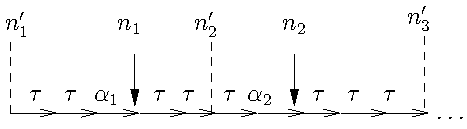
\includegraphics[width=6cm]{XFIG/proof-explain}
\end{center}\caption{Composition of the subsequences}\label{figproof}
\end{figure}

 We can decompose each of the $n+1$ subsequences in the following way (see Figure~\ref{figproof}).
For $k\in [0..n]$ the position of the $k^{\text{th}}$ visible action is  $n_k$. For $l\in [1..n]$,  $n'_l$ is any index between $n_{l-1}$ and $n_l$, additionally $n'_0=0$ and $n'_{n+1}=n_1+n_2+3$. We obtain $n+1$ subsequences  made of the following OTs, for all $k\in [0..n]$ :\\
\begin{small}
$\forall p\! \in\! [n'_{k}..(n_k\!-\!1)] Q\models{\openrule
			{
				\beta_{pj}^{j\in J\cap\Holes(Q)}, {{\Pred\,''_{p}}},  
				{{\Post\,''_{p}}}}
				{\ostate{v_{pl}^{l\in L_Q}} \OTarrow {\tau}
				\ostate{v_{(p+1)l}^{l\in L_Q}}}
				}%\]
,\quad
Q\models{\openrule
			{
				\beta_{n_k j}^{j\in J\cap\Holes(Q)}, {{\Pred\,''_{n_k}}},  
				{{\Post\,''_{n_k}}}}
				{\ostate{v_{n_kl}^{l\in L_Q}} \OTarrow {\alpha_{{n_k}}}
				\ostate{v_{(n_k+1)l}^{l\in L_Q}}}
				}%\]
$
\end{small}
and\\
\begin{small}
$\forall p \in [(n_k\!+\!1)..(n'_{k+1}\!-\!1)]\,\, Q\models{\openrule
			{
				\beta_{pj}^{j\in J\cap\Holes(Q)}, {{\Pred\,''_{p}}},  
				{{\Post\,''_{p}}}}
				{\ostate{v_{pl}^{l\in L_Q}} \OTarrow {\tau}
				\ostate{v_{(p+1)l}^{l\in L_Q}}}
				}%\]
$
\end{small}
\\ 
Thereafter, by Lemma \ref{lem-rel-OT-WOT} we can deduce the following weak open transition:
\begin{mathpar}
Q\models{\openrule
			{
			(\gamma_{kj})^{j\in J\cap\Holes(Q)},  {{\Pred_k}},  
				{{\Post_k}}}
			{\ostate{v_{kl}^{l\in L_Q}} \OTWeakarrow {\alpha'_{k}}
				\ostate{(v_{kl}')^{l\in L_Q}}}
		}%\]
\end{mathpar}
With:
$\forall l \in L_Q. v_{kl}=v_{(n'_{k})l} \wedge v_{kl}'=v_{(n'_k)l}$\\
$\alpha_k'=\alpha_{n_k}\displaystyle{\subst{\bigotimes_{j=n_k-1}^{n'_{k}}\!\!\Post\,''_{j}}}$\\
$\displaystyle{\gamma_{kj}^{j\in J\cap\Holes(Q)} }=\displaystyle{\mybigdotcup_{i=n'_{k}}^{(n_k\!-\!1)} \vis{{\beta_{ij}^{j\in J\cap\Holes(Q)}}\subst{\bigotimes_{l=i-1}^{n'_{k}}\!\!\!\Post\,''_{l}}}\dotcup \vis{{\beta_{n_k j}^{j\in J\cap\Holes(Q)}}\subst{\bigotimes_{l=n_k-1}^{n'_{k}}\!\!\!\Post\,''_{l}}}} \dotcup\\
{}~~\qquad \qquad\qquad\mybigdotcup_{i=n_k+1}^{n'_{k+1}-1}
\vis{{\beta_{ij}^{j\in J\cap\Holes(Q)}} \subst{\bigotimes_{l=i-1}^{n_k\!+\!1}\!\Post\,''_{l}\shortotimes\Post\,''_{n_k}\shortotimes\!\!\bigotimes_{l=n_k-1}^{n'_{k}}\!\!\!\Post\,''_{l}} }\\
%
\Pred_k=\bigwedge_{i=n'_{k}}^{n_k\!-\!1}\!\!\Pred\,''_{i}\subst{\bigotimes_{j=i-1}^{n'_{k}}\!\!\Post\,''_{j}}\land\Pred\,''_{n_k} \subst{\bigotimes_{j=n_k-1}^{n'_{k}}\!\!\Post\,''_{j}}\land\\ 
{}~\qquad\quad\bigwedge_{i=n_k+1}^{n'_{k+1}-1}\!\!\!\Pred\,''_{i}\subst{\bigotimes_{j=i-1}^{n'_{k}}\!\!\!\Post\,''_{j}\shortotimes\Post\,''_{n_k}\shortotimes\!\!\bigotimes_{j=n_k-1}^{n'_{k}}\!\!\!\Post\,''_{j}}
\\
\Post_k= \bigotimes_{j=n'_{k+1}-1}^{n'_{k}}\!\!\Post\,''_{j}$\\


\noindent Note that for all $k\in[0..n-1]$, $v_{kl}'=v_{(k+1)l}$,  $v_{0l}=s_{0l}=s_l$, and $v'_{nl}=v_{(n_1+n_2+3) l}=u_{(n_2+1) l} = s'_l$.

\noindent By definition of $\Post_k$, we have $\displaystyle{\bigotimes_{j=n'_{k}-1}^{0}\!\!\Post\,''_{j} = \bigotimes_{j=k-1}^{0}\!\!\Post_{j}}$.
%In this case, the number of weak open transitions
%might not be exactly the number of open transitions that take part in the reduction but something smaller, thus the resulting set of weak open transitions could also be smaller.\\
Consequently,  we have:
\[\alpha_{n_k}\displaystyle{\subst{\!\bigotimes_{j=n_k-1}^{0}\!\!\!\Post\,''_{j}}} =
\alpha_{n_k}\displaystyle{\subst{\!\bigotimes_{j=n_k-1}^{n'_{k}}\!\!\!\Post''_{j}\otimes\!\!\!\bigotimes_{j=n'_{k}-1}^{0}\!\!\!\Post\,''_{j}}} = \alpha_k'\displaystyle{\subst{\!\bigotimes_{j=n'_{k}-1}^{0}\!\!\!\Post\,''_{j}}} = 
\alpha_k'\displaystyle{\subst{\!\bigotimes_{j=k-1}^{0}\!\!\Post_{j}}}\]
With~\ref{eqproofbeta}, we now have (the actions $\alpha'_p$ correspond to the observable actions, $\alpha_k$): 
\begin{eqnarray*}
\Pred_\beta &\iff& \gamma_{j_0}=
\mybigdotcup_{p=0}^{p=n_1+n_2+2}
\vis{\alpha_{p}\subst{\bigotimes_{j=p-1}^{0}\!\!\Post_{j}}}\\
%&\iff&\gamma_{j_0}=
%\mybigdotcup_{p=0}^{p=n_1+n_2+2}
%\vis{\alpha_{p}\subst{\bigotimes_{j=p-1}^{n'_p}\!\!\Post_{j}}\subst{\bigotimes_{j=n'_p-1}^{0}\!\!\Post_{j}}}\\
%\vis{[\alpha_{p}\subst{\bigotimes_{j=p-1}^{0}\!\!\Post_{j}}|p\in[0..n_1+n_2+2]]}\\
%&\iff& \gamma_{j_0}=
%\vis{[\alpha'_{p}\subst{\bigotimes_{j=p-1}^{0}\!\!\Post_{j}}|p\in[1..n]]}\\
&\iff& \gamma_{j_0}=
[\alpha'_{p}\subst{\bigotimes_{j=p-1}^{0}\!\!\Post_{j}}|p\in[0..n]]
\end{eqnarray*}

 
We need now to show that this set of WOT verifies the conditions of the lemma, i.e. it is a set of WOT of the form:
\[	Q\models{\openrule
			{
				\gamma_{p j}^{j\in J_p}, \Pred_p,  
				\Post_p}
			{\ostate{s_{p i}^{i\in L_Q}} \OTWeakarrow {\alpha_p}
				\ostate{s_{(p+1) i}^{\,i\in L_Q}}}
		}\]
With
\[  \bigcup_{p=0}^nJ_{p} = J\cap\Holes(Q) \qquad\text{trivial}\]
\[ \gamma_j^{j\in J\cap\Holes(Q)}= \mybigdotcup_{p=0}^n (\gamma_{p j}^{j\in J_p})\subst{\bigotimes_{i=p-1}^{0}\Post_i)}\]
Indeed we have:
\begin{equation*}
\begin{split}
\gamma_j^{j\in J}=&\mybigdotcup_{i=0}^{m_1} \vis{\set{\beta_{1i}}\subst{\bigotimes_{j=i-1}^{0}\!\! \Post_{1j}}}\dotcup  \vis{\set{\beta_2}\subst{\bigotimes_{j=m_1}^{0}\Post_{1j}}} \dotcup\\& \mybigdotcup_{i=0}^{m_2} \vis{\set{\beta_{3i}} \subst{\bigotimes_{j=i-1}^{0}\!\Post_{3j}\shortotimes\Post_2\shortotimes\bigotimes_{j=m_1}^{0}\!\!\Post_{1j}} }\\
\end{split}\end{equation*}

And thus, because $\beta_{pj}^{j\in J\cap \Holes(Q)}$ are equal to the concatenation of  $(\beta'_{1pj})^{j\in J\cap \Holes(Q)}$, $(\beta'_{2j})^{j\in J\cap \Holes(Q)}$, and $(\beta_{3pj}')^{j\in J\cap \Holes(Q)}$ (re-indexed because we skipped some transitions), and additionally $(\beta_{1pj}')^{j\in J\cap \Holes(Q)}$, $(\beta_{2j}')^{j\in J\cap \Holes(Q)}$, and $(\beta_{3pj}')^{j\in J\cap \Holes(Q)}$ are identical to the hole labels $\beta_{1kj}^{j\in J\cap \Holes(Q)}$, $\beta_{2j}^{j\in J\cap \Holes(Q)}$, and $\beta_{3kj}^{j\in J\cap \Holes(Q)}$ (re-indexed) when $Q$ moves\footnote{more precisely, when $Q$ moves either $\beta_{1kj}^{j\in J\cap \Holes(Q)}$ is not empty  and thus $(\beta_{1pj}')^{j\in J\cap \Holes(Q)}=\beta_{1kj}^{j\in J\cap \Holes(Q)}$, or both are empty if the holes of $Q$ perform no action}. We can assert a similar equality on postconditions, i.e. between $\Post\,''_p$ and $\Post\,''_{1k}$, $\Post\,''_{2}$, $\Post\,''_{3k}$ where $\Post\,''_{1p}$ is the restriction of $\Post_{1p}$ over variables of $\Leaves(Q)$ (see initial decomposition, case 1, 2, and 3 above). Overall, we have

$\forall i \in L_Q.\, s_{(n+1) i} = s_i'\land s_{0 i} = s_i$ (see above)\\
{\scriptsize \begin{equation*}
\begin{split}
\gamma_j^{j\in J\cap \Holes(Q)}&=\mybigdotcup_{i=0}^{m_1} \vis{\set{(\beta_{1i}')}\subst{\bigotimes_{j=i-1}^{0}\!\! \Post''_{1j}}}\dotcup  \vis{\set{\beta'_2}\subst{\bigotimes_{j=m_1}^{0}\Post''_{1j}}} \dotcup \mybigdotcup_{i=0}^{m_2} \vis{\set{\beta'_{3i}} \subst{\bigotimes_{j=i-1}^{0}\!\Post''_{3j}\shortotimes\Post''_2\shortotimes\bigotimes_{j=m_1}^{0}\!\!\Post''_{1j}} }\\
&=\mybigdotcup_{k=0}^n \left( \mybigdotcup_{i=n'_k}^{n'_{k+1}-1}\vis{\beta_{ij}^{j\in J\cap \Holes(Q)}\subst{\bigotimes_{j=i-1}^{n'_k}\!\!\Post''_{j}\bigotimes_{j=n'_k-1}^{0}\!\!\Post''_{j}}}\right)\\
&=\mybigdotcup_{k=0}^n \left( \gamma_{kj}^{j\in J\cap \Holes(Q)}\subst{\bigotimes_{j=k-1}^{0}\!\!\Post_{k}}\right)
\end{split}\end{equation*}
}
$\Pred = \displaystyle{\Pred\,'
		\land \!\!\bigwedge_{p=0}^n((\alpha_p\subst{\bigotimes_{i=p-1}^{0}\Post_i)} = \beta_p\land (\Pred_p\subst{\bigotimes_{i=p-1}^{0}\Post_i)} )}$\\
Indeed,
\begin{small}
\begin{equation*}
\begin{split}
\Pred&\iff\bigwedge_{i=0}^{m_1}\Pred_{1i}\subst{\bigotimes_{j=i-1}^{0}\!\!\Post_{1j}}\land\Pred_2 \subst{\bigotimes_{j=m_1}^{0}\!\!\Post_{1j}}\land
\bigwedge_{i=0}^{m_2}\Pred_{3i}\subst{\bigotimes_{j=i-1}^{0}\!\!\Post_{3j}\shortotimes\Post_2\shortotimes\bigotimes_{j=m_1}^{0}\!\!\Post_{1j}}\\
&\iff\bigwedge_{i=0}^{m_1}\left(\Pred\,'_{1i}
		\land {\Pred\,''_{1i}}\land \alpha_{1i}=\beta_{1ij_0}\right)\subst{\bigotimes_{j=i-1}^{0}\!\!\Post_{1j}} \\
&\qquad\land\left(\Pred\,'_{2}
		\land {\Pred\,''_{2}}\land \alpha_{2}=\beta_{2j_0}\right)\subst{\bigotimes_{j=m_1}^{0}\!\!\Post_{1j}}\\
&\qquad\land\bigwedge_{i=0}^{m_2} \left(\Pred\,'_{3i}
		\land {\Pred\,''_{3i}}\land \alpha_{3i}=\beta_{3ij_0}\right) \subst{\bigotimes_{j=i-1}^{0}\!\!\Post_{3j}\shortotimes\Post_2\shortotimes\bigotimes_{j=m_1}^{0}\!\!\Post_{1j}}\\
&\iff\bigwedge_{i=0}^{m_1}\left((\Pred\,'_{1i}\subst{\bigotimes_{j=i-1}^{0}\!\!\Post\,'_{1j}})
		\land ({\Pred\,''_{1i}}\subst{\bigotimes_{j=i-1}^{0}\!\!\Post\,''_{1j}})\land (\alpha_{1i}=\beta_{1ij_0})\subst{\bigotimes_{j=i-1}^{0}\!\!\Post_{1j}}\right) \\
&\qquad\land \left(\Pred\,'_{2}\subst{\bigotimes_{j=m_1}^{0}\!\!\Post_{1j}}
		\land {\Pred\,''_{2}} \subst{\bigotimes_{j=m_1}^{0}\!\!\Post_{1j}} \land (\alpha_{2}=\beta_{2j_0})\subst{\bigotimes_{j=m_1}^{0}\!\!\Post_{1j}} \right) \\
&\qquad\land\bigwedge_{i=0}^{m_2} \Bigg(\Pred\,'_{3i} \subst{\bigotimes_{j=i-1}^{0}\!\!\Post_{3j}\shortotimes\Post_2\shortotimes\bigotimes_{j=m_1}^{0}\!\!\Post_{1j}} 
		\land {\Pred\,''_{3i}} \subst{\bigotimes_{j=i-1}^{0}\!\!\Post_{3j}\shortotimes\Post_2\shortotimes\bigotimes_{j=m_1}^{0}\!\!\Post_{1j}}  \\
		 & \qquad \land (\alpha_{3i}=\beta_{3ij_0}) \subst{\bigotimes_{j=i-1}^{0}\!\!\Post_{3j}\shortotimes\Post_2\shortotimes\bigotimes_{j=m_1}^{0}\!\!\Post_{1j}}\Bigg)  \\
&\iff \Pred\,'\land\bigwedge_{k=0}^n\Pred_k\subst{\bigotimes_{j=k-1}^{0}\!\!\Post_{j}}\land\Pred_\beta
\\&\iff \Pred\,'\land\bigwedge_{k=0}^n\Pred_k\subst{\bigotimes_{j=k-1}^{0}\!\!\Post_{j}}\land
(\gamma_{j_0}=[\alpha'_{i}\subst{\bigotimes_{j=i-1}^{0}\!\!\Post_{j}}|i\in[0..n]])
\end{split}\end{equation*}
\end{small}
which is exactly what is needed.\\
Finally we have~~
$\Post=\displaystyle{\Post\,' \uplus \bigotimes_{p=n}^0
		\Post_p}$\quad
because
\begin{equation*}
\begin{split}
\Post&=\bigotimes_{j=m_2}^{0}\!\!\Post_{3j}\shortotimes\Post_2\shortotimes\bigotimes_{j=m_1}^{0}\!\!\Post_{1j}\\
&=\bigotimes_{j=m_2}^{0}\!\!\Post\,'_{3j}\shortotimes\Post\,'_2\shortotimes\bigotimes_{j=m_1}^{0}\!\!\Post\,'_{1j} \uplus \bigotimes_{j=m_2}^{0}\!\!\Post\,''_{3j}\shortotimes\Post\,''_2\shortotimes\bigotimes_{j=m_1}^{0}\!\!\Post\,''_{1j}\\
&=\Post\,' \uplus \bigotimes_{j=n'_{n+1}-1}^{0}\!\!\Post\,''_{j}
\end{split}
\end{equation*}
%
%Consequently, we have $n$ weak open transitions  $\symb{WOT}_k$ such that $k\in [1..n]$.
%Therefore, we can conclude that we have for all $k\in [1..n]$:  
%\begin{mathpar}
%Q\models{\openrule
%			{
%			\gamma_{kj}^{j\in J_k}, {\Pred_k}, {\Post_k}}
%			{\ostate{s_{pl}^{l\in L_Q}} \OTWeakarrow {\alpha'_{k}}
%				\ostate{s_{(p+1)l}^{l\in L_Q}}}
%		}%\]
%\end{mathpar}
%
%%By considering $n=m_1+m_2+2$,  and $\forall p \in [0..n]$: \\
%%$\Pred_{p}= \left\{
%% \begin{array}{ll}
%%\Pred_{1p} & \mbox{if }p<m_1\\
%%\Pred_{2} & \mbox{if } p=m_1\\
%%\Pred_{1(p-m_1)} & \mbox{if }p\geq m_1\\
%%\end{array}
%%\right. 
%%\quad$
%% $\qquad
%%\Post_{p}= \left\{
%% \begin{array}{ll}
%%\Post_{1p} & \mbox{if }p<m_1\\
%%\Post_{2} & \mbox{if } p=m_1\\
%%\Post_{1(p-m_1)} & \mbox{if }p\geq m_1\\
%%\end{array}
%%\right. 
%%$\\
%%and similarly for $\beta_p$. Thus, we can rewrite $\gamma$ given in the hypothesis as: \\
%%$\set{\gamma}= \displaystyle{\mybigdotcup_{p=0}^{n}
%%\vis{\set{\beta_{p}}}\subst{\bigotimes_{p=n}^{0} \Post_{p}}}$\\
%Furthermore, still by hypothesis we have:\\
%$\Pred=\displaystyle{\bigwedge_{i=0}^{m_1}\Pred_{1i}\subst{\bigotimes_{j=i-1}^{0}\!\!\Post_{1j}}\land\Pred_2 \subst{\bigotimes_{j=m_1}^{0}\!\!\Post_{1j}} }\land \\
%~\qquad \quad \bigwedge_{i=0}^{m_2}\Pred_{3i}\subst{\bigotimes_{j=i-1}^{0}\!\!\Post_{3j}\shortotimes\Post_2\shortotimes\bigotimes_{j=m_1}^{0}\!\!\Post_{1j}}$\\
%By replacing $\Pred_{1i}$,  $\Pred_2$, and $\Pred_{3i}$ by their equivalent formula obtained from cases 1, 2 and 3 we have:\\
%$\Pred =\displaystyle{\bigwedge_{i=0}^{m_1}({\Pred'_{1i}}
%		\land {\Pred''_{1i}}\land \alpha_{1i}=\beta_{1ij_0}) \bigotimes_{j=i-1}^{0}\subst{\Post_{1j}}\land}\\
%~~\qquad\qquad({\Pred'_2}\land {\Pred''_2}\land \alpha_2=\beta_{2j_0})	\bigotimes_{i=m_1}^{0}\subst{\Post_{1i}}\land\\
%~~\qquad\qquad\bigwedge_{i=0}^{m_2} ({\Pred'_{3i}}\land {\Pred''_{3i}}\land \alpha_{3i}=\beta_{3ij_0})
%\subst{\bigotimes_{j=i-1}^{0}\!\!\Post_{3j}\shortotimes\Post_2\shortotimes\bigotimes_{j=m_1}^{0}\!\!\Post_{1j}}$\\
%By distribution of the substitution operation over the logical operator we reformulate as:\\
%$\Pred= \displaystyle{\big(\bigwedge_{i=0}^{m_1}
%{\Pred'_{1i}}\bigotimes_{j=i-1}^{0}\subst{{\Post'_{1j}}}\big)
%\land{\Pred'_2}\bigotimes_{i=m_1}^{0}\subst{{\Post'_{1i}}}\land} \\
%~~\qquad\qquad\bigwedge_{i=0}^{m_2}{\Pred'_{3i}}\bigotimes_{j=i-1}^{0}\subst{{\Post'_{3j}}}\subst{{\Post'_2}}\bigotimes_{j=m_1}^{0}\subst{{\Post'_{1j}}} \land\\	
%~\qquad\qquad\bigwedge_{i=0}^{m_1}({\Pred''_{1i}}\land \alpha_{1i}=\beta_{1ij_0}) \bigotimes_{j=i-1}^{0}\subst{\Post_{1j}}\land({\Pred''_2}\land \alpha_2=\beta_{2j_0})	\bigotimes_{i=m_1}^{0}\subst{\Post_{1i}}\land\\
%~\qquad\qquad\bigwedge_{i=0}^{m_2} ({\Pred''_{3i}}\land \alpha_{3i}=\beta_{3ij_0})\bigotimes_{j=i-1}^{0}\subst{\Post_{3j}}\subst{\Post_2}  \bigotimes_{i=m_1}^{0}\subst{\Post_{1i}}
%$\\		
%Thus, we can write the formula as follows:\\
%$\Pred= \Pred\,' \wedge \displaystyle{\bigwedge_{p=0}^{n}}((\alpha_p= \beta_{pj_0}\land \Pred_p)\bigotimes_{i=p-1}^{0}\Post_i)$\\
%We proceed the same way with the postcondition,  we have:\\
%$\Post=\displaystyle{\bigotimes_{j=m_2}^{0}\!\!\Post_{3j}\shortotimes\Post_2\shortotimes\bigotimes_{j=m_1}^{0}\!\!\Post_{1j}}$\\
%By replacing ${\Post_{1i}}$,  $\Post_2$, and ${\Post_{3i}}$ their values obtained from the cases 1, 2, and 3, and because the ${\Post'_i}$ and ${\Post''_i}$ are independent (the ${\Post'_i}$ concern the leaves of $P$ while the ${\Post''_i}$ concern the leaves of $Q$), we obtain:\\
%$\Post= \displaystyle{\bigotimes_{i=m_2}^{0}\subst{{\Post'_{3i}}\uplus 
%		{\Post''_{3i}}} \subst{{\Post'_2}\uplus 
%		{\Post''_2}} \bigotimes_{j=m_1}^{0}\subst{ {\Post'_{1i}}\uplus 
%		{\Post''_{1i}}}}\\
%~~\qquad= \bigotimes_{i=m_2}^{0}{\Post'_{3i}}\subst{{\Post'_2}}\bigotimes_{j=m_1}^{0}\subst{{\Post'_{1j}}} \uplus \bigotimes_{i=m_2}^{0}{\Post''_{3i}}\subst{{\Post''_2}}\bigotimes_{j=m_1}^{0}\subst{{\Post''_{1j}}} \\
%~~\qquad= \Post' \uplus \bigotimes_{j=n}^{0} \Post_j $\\
%\qed
\end{proof}

\begin{lemma}[Weak open transition composition]\label{lem-Weakcompose1} Suppose that we have a weak open automaton such that the WOTs cannot observe silent actions (see Definition \ref{def:Non-ObsTau}).
	Suppose $j_0\in J$  and:\\[-1ex]
\begin{mathpar}
%\[
P\models{\openrule
	{
		\beta_j^{j\in J}, 
		\Pred,  
		\Post}
	{\ostate{s_i^{i\in L}} \OTarrow {\alpha}
		\ostate{(s_i')^{\, i\in L}}}
}
\quad\text{~~and~~}\quad
Q\models{\openrule
	{
		\set{\gamma},
		 \Pred_Q,  
		\Post_Q}
	{\ostate{s_{i}^{i\in L_Q}} \OTWeakarrow {\alpha_Q}
		\ostate{(s'_{i})^{\, i\in L_Q}}}
}%\]
\end{mathpar}
Let\\[-3ex] 
\begin{mathpar}
%J_Q=\displaystyle{\bigcup_{t=0}^nJ_{t}}
%\qquad
\Pred\,'=\Pred\land (\beta_{j_0}=\alpha_Q\land \Pred_Q) \quad\text{~~and~~}\quad
%\forall j\in J_t,\,\gamma_j= \displaystyle{\mybigdotcup_{t=0}^n \gamma_{t j}}\text{\quad and\quad}
\Post\,'=\Post\uplus\Post_Q
\end{mathpar}
Then, we have\\[-3ex]
	\[ P[Q]_{j_0}  
	\models
	{\openrule
		{
			\set{\gamma}\uplus\vis{\beta_j^{j\in J\setminus \{j_0\}}}, 
			\Pred\,',  \Post\,'
			 }
		{\ostate{s_i^{i\in L\uplus L_Q}} \OTWeakarrow {\alpha}
			\ostate{(s_i')^{\, i\in L\uplus L_Q}}}
	}
	\]
\end{lemma}
\begin{proof}
By  Lemma \ref{lem-rel-OT-WOT} we can decompose the WOT of $Q$ into  a series of $k+1$ and $k'+1$ tau open transitions and an observable open transition:
\begin{mathpar}
\forall h\!\in\![0..k].Q\models\openrule
    {\set{\beta_{1h}},\Pred_{1h},\Post_{1h}   }
         {\ostate{{(s_{1h})}} \OTarrow {\tau} \ostate{{(s_{1(h+1)})}}}, \quad
Q\models{\openrule
	{
		\set{\beta_2},
		 \Pred_2,  
		\Post_2}
	{\ostate{s_{20}}\OTarrow {\alpha'_Q}
		\ostate{s_{21}}}
}, \\ \quad\text{~~and~~}\quad 
\forall h \in [0..k'].Q\models\openrule
         {
           \set{\beta_{3h}},\Pred_{3h}, \Post_{3h}}
         { \ostate{(s_{3h})} \OTarrow {\tau} \ostate{(s_{3(h+1)})}}
\end{mathpar}
such that

\begin{small}
$s_i^{i\in L_Q}=s_{10} \wedge s_{1(k+1) i}=s_{20} \wedge  s_{21}= s_{30} \wedge s_{3(k'+1) i}={s'}_i^{i\in L_Q}$
\begin{align*}
\alpha_Q=&\alpha'_Q\displaystyle{\subst{\bigotimes_{j=k}^{0}\Post_{1j}}}\\
\set{\gamma}=&\mybigdotcup_{h=0}^k \vis{\set{\beta_{1h}}\subst{\bigotimes_{j=h-1}^{0}\!\! \Post_{1j} } }  \dotcup  \vis{\set{\beta_2}\subst{\bigotimes_{j=k}^{0}\Post_{1j}}} \dotcup%\\
		%&
 \mybigdotcup_{h=0}^{k'} \vis{\set{\beta_{3h}} \subst{\bigotimes_{j=h-1}^{0}\!\!\Post_{3j}\shortotimes\Post_2\shortotimes\bigotimes_{j=k}^{0}\Post_{1j}} }\\
\Pred_Q=&\bigwedge_{h=0}^{k}\!\big(\Pred_{1h}\subst{\bigotimes_{j=h-1}^{0}\Post_j^1}\big)\land \Pred_2\subst{\bigotimes_{h=k}^{0}\Post_{1h}}\land\\
&		\bigwedge_{h=0}^{k'}\!\Pred_{3h}\subst{\bigotimes_{j=h-1}^{0}{\Post_{3j}}\otimes{\Post_2}  \otimes\bigotimes_{h=k}^{0}\Post_{1h}}\\
\Post_Q=&\bigotimes_{h=k'}^{0}\Post_{3h}\otimes\Post_2\otimes\bigotimes_{j=k}^{0}\Post_{1j}
\end{align*}


\end{small}
\begin{enumerate}

\item For the first $k$ open tau transitions, by Definition \ref{def:Non-ObsTau} $P$ can necessarily make a tau open transition if the hole indexed $j_0$ makes a tau action. So by Lemma \ref{lem-compose} we obtain $k$ open transitions in the form: 
\[P[Q]_{j_0}\!\models		
\openrule
    {
       \set{\beta_{1h}},{\Pred_{1h}},{\Post_{1h}}   }
         {\ostate{s_{1h}\uplus s^{i\in L}_{i} } \OTarrow {\tau} \ostate{s_{1(h+1)}\uplus s^{i\in L}_{i}}}\]


\item For the observable open transition.  By Lemma \ref{lem-compose} with the lemma hypotheses we obtain:\\ 
	\[ P[Q]_{j_0}  
	\models
	{\openrule
		{
			{\beta_{j}}^{(j\in J\setminus\{j_0\})} \uplus \set{\beta_2}, 
			\Pred\land\Pred_2\land \alpha_Q=\beta_{j_0 },  
			\Post\uplus \Post_2}
{\ostate{s^{i\in L}_{i}\uplus s_{20}} \OTarrow {\alpha} \ostate{{s'}^{i\in L}_{i}\uplus s_{21}}}
	}
	\]

%
%\[P[Q]_{j_0}\!\models		
%\openrule
%    {
%       {\beta^i_{p j}}^{(j\in J\setminus\{j_0\})} \uplus \set{\beta_2},{\Pred_p}\!\!'',{\Post_p}\!\!''   }
%         {\ostate{s^{i\in L \uplus L_Q}_{pi}} \OTarrow {\alpha} \ostate{s^{i\in L\uplus L_Q }_{(p+1)i}}}\] \\
% such that  ${\Pred_p}\!\!'' \iff {\Pred_p}
%		\land {\Pred_p}\!\!'\land \alpha_t=\beta_{j_0}$, ${\Post_p}\!\!''={\Post_p}\uplus 
%		{\Post_p}\!\!'$\\ 
\item We proceed in the same way as the first item for $k'$ last weak open transitions, and we obtain $k'$ open tau transitions.
\end{enumerate}

Using Lemma \ref{lem-rel-OT-WOT}, from cases $(1)$, $(2)$ and $(3)$ we get: 
\[P[Q]_{j_0}\!\models		
\openrule
    {
\set{\gamma_c}, \Pred_c,
\Post_c}
         {\ostate{s_{10}\uplus s^{i\in L}_{i}} \OTWeakarrow {\alpha'} 
	\ostate{{{s'}^{i\in L}_{i}\uplus s_{3(k'+1)}}}}\] 
where ~~
$\alpha'=\alpha\displaystyle{\subst{\bigotimes_{j=k}^{0}\Post_{1j}}}$
and $\alpha=\alpha'$  because $\Post_{1j}$ acts on variables of $Q$ and $\alpha$ contains only variables of $P$.\\
$\displaystyle{
\set{\gamma_c}=\mybigdotcup_{h=0}^k \vis{\set{\beta_{1h}}\subst{\bigotimes_{i=h-1}^{0}\!\! \Post_{1i} } }  \dotcup  \vis{({\beta_{j}}^{(j\in J\setminus\{j_0\})} \uplus \set{\beta_2})\subst{\bigotimes_{i=k}^{0}\Post_{1i}}} \dotcup}$ \\ 
${}~~\hspace{1.8em}\displaystyle{\mybigdotcup_{h=0}^{k'} \vis{\set{\beta_{3h}} \subst{\bigotimes_{i=h-1}^{0}\!\!\Post_{3i}\shortotimes\Post_2\shortotimes\bigotimes_{i=k}^{0}\Post_{1i}} }}$\\
${}~~\hspace{0.6em}=\set{\gamma}\uplus\vis{\beta_j^{\in J\setminus \{j_0\}}} \quad$  because $\Post_{1j}$  does not act on variables of $\beta_j$.  \\
\begin{small}
$\Pred_c=\begin{array}[t]{l}\displaystyle\bigwedge_{h=0}^k{\Pred_{1h}}\subst{\bigotimes_{i=h-1}^{0}\Post_{1i}}\land
\left(Pred\land\Pred_2\land \alpha'_Q=\beta_{j_0 }\right)\subst{\bigotimes_{i=k}^{0}{\Post_{1i}}}\land\\\displaystyle
\bigwedge_{h=0}^{k'}{\Pred_{3h}}\subst{\bigotimes_{i=h-1}^{0}{\Post_{3i}}\shortotimes({\Post\uplus \Post_2})\shortotimes\bigotimes_{i=k}^{0}{\Post_{1i}}}
\end{array}
$\\
$\Post_c=\displaystyle{(\bigotimes_{i=k'}^{0}{\Post_{3i}})\shortotimes({\Post\uplus \Post_2})\shortotimes\bigotimes_{i=k}^{0}{\Post_{1i}}}$
\end{small}

\noindent Note that we have $s_i^{i\in L_Q}=s_{10} \wedge s_{1(k+1) i}=s_{20} \wedge  s_{21}= s_{30} \wedge s_{3(k'+1) i}={s'}_i^{i\in L_Q}$

Note also that $\Post$ only acts on variables of $P$ while $\Post_{1i}$ only acts on state variables of $Q$. We conclude on predicate and posts as follows\footnote{$\Post_{1i}$ only has an effect on variables of $Q$ and thus does not modify $\Pred$ or $\beta_{j_0}$}:
\begin{equation*}
\begin{split}
\Pred_c&=\Pred_Q\land\Pred\subst{\bigotimes_{i=k}^{0}{\Post_{1i}}}\land
(\alpha'_Q=\beta_{j_0})\subst{\bigotimes_{i=k}^{0}{\Post_{1i}}}\\
&=\Pred_Q\land\Pred\land \alpha_Q=\beta_{j_0}\\[.3ex]
\Post_c&=\Post\uplus\Post_Q \\[-3ex]
\end{split}
\end{equation*}
\end{proof}

\begin{lemma}[Weak open transition composition]\label{lem-Weakcompose} Suppose that we have a weak open automaton such that the WOTs cannot observe silent actions (see Definition \ref{def:Non-ObsTau}). Suppose $j_0\in J$ and $\gamma_{j_0}=[\beta_0..\beta_n]$ and additionally:\\[-2ex]
\begin{mathpar}
%\[
P\models{\openrule
	{
		\gamma_j^{j\in J}, 
		\Pred,  
		\Post}
	{\ostate{s_i^{i\in L}} \OTWeakarrow {\alpha}
		\ostate{s_i'^{\, i\in L}}}
}\\
\text{~~and for all $p\in[0..n]$~~}
Q\models{\openrule
	{
		\gamma_{pj}^{j\in J_p},
		 \Pred_p,  
		\Post_p}
	{\ostate{s_{pi}^{i\in L_Q}} \OTWeakarrow {\alpha_p}
		\ostate{s_{(p+1) i}^{\, i\in L_Q}}}
}%\]
\end{mathpar}

Let 
\begin{mathpar}
J_Q=\displaystyle{\bigcup_{p=0}^nJ_{p}}
\qquad
\Pred\,'=\Pred\land \bigwedge_{p=0}^{n}(\alpha_t=\beta_t\land \Pred_t)\bigotimes_{i=p-1}^{0}\Post_i
\\
\forall j\in J_p,\,\gamma_j= \displaystyle{\mybigdotcup_{p=0}^n \gamma_{p j}\subst{\bigotimes_{k=p}^{0}{\Post_k}}}\text{\quad and\quad}
\Post\,'=\Post\uplus\bigotimes_{p=n}^{0}
		\Post_p
\\
\forall{i\in L_Q}.\,s_i=s_{0i} \text{\quad and \quad} \forall {i\in L_Q}.\,s'_i=s_{(n+1) i}
\end{mathpar}
Then, we have\\[-2ex]
	\[ P[Q]_{j_0}  
	\models
	{\openrule
		{
			\gamma_j^{j\in (J\setminus\{j_0\}) \uplus J_Q}, 
			\Pred\,',  \Post\,'
			 }
		{\ostate{s_i^{i\in L\uplus L_Q}} \OTWeakarrow {\alpha}
			\ostate{s_i'^{\, i\in L\uplus L_Q}}}
	}
	\]
\end{lemma}

\begin{proof} Suppose we have:
\begin{mathpar}
%\[
P\models{\openrule
	{
		\gamma_j^{j\in J}, 
		\Pred,  
		\Post}
	{\ostate{s_i^{i\in L}} \OTWeakarrow {\alpha}
		\ostate{s_i'^{\, i\in L}}}
}
\end{mathpar}
By Lemma \ref{lem-rel-OT-WOT} this implies the following: \\			
%\begin{mathpar}
\begin{small}
$\forall p\!\in\![0..m_1].P\models\openrule
    {{\beta_{1pj}^{j\in J_{1p}}},\Pred_{1p},\Post_{1p}   }
         {\ostate{{(s_{1pi})}^{i\in L}} \OTarrow {\tau} \ostate{{(s_{1(p+1)i})}^{i\in L}}},  \quad
P\models\openrule
         {\beta_{2j}^{j\in J_2},\Pred_2,\Post_2 }
         {\ostate{({s_{20i}})^{i\in L}} \OTarrow {\alpha'} \ostate{({s_{21i}})^{i\in L}}} $ 
\\
and  $\forall p \in [0..m_2].P\models\openrule
         {
           \beta_{3pj}^{j\in J_{3p}},\Pred_{3p}, \Post_{3p}}
         { \ostate{(s_{3pi})^{i\in L}} \OTarrow {\tau} \ostate{(s_{3(p+1)i})^{i\in L}}}$
\end{small}
~~\\
%\end{mathpar}
\noindent where for all $i\in L$:\\
$s_i=s_{10 i} \wedge s_{1(m_1+1) i}=s_{20i} \wedge  s_{21i}= s_{30 i} \wedge s_{3(m_2+1) i}=s'_i$\\
$\alpha=\alpha'\displaystyle{\subst{\bigotimes_{j=m_1}^{0}\Post_{1j}}}$ \\
%\begin{multline*}
$\gamma_j^{j\in J}=\displaystyle{\mybigdotcup_{i=0}^{m_1} \vis{{\beta_{1ij}^{j\in J_{1p}}}\subst{\bigotimes_{k=i-1}^{0} \Post_{1k} } }  \dotcup \, \vis{{\beta_{2j}^{j\in J_{2}}}\subst{\bigotimes_{k=m_1}^{0}\Post_{1k}}}}\, \dotcup\\
{}~\qquad\quad \mybigdotcup_{i=0}^{m_2} \vis{\beta_{3ij}^{j\in J_{3p}} \subst{\bigotimes_{k=i-1}^{0}\Post_{3k}\shortotimes\Post_2\shortotimes\bigotimes_{k=m_1}^{0}\Post_{1k}}}$\\
%\end{multline*}
%\begin{multline*}
$\Pred=\displaystyle{\bigwedge_{p=0}^{m_1}\!\big(\Pred_{1p}\subst{\bigotimes_{j=p-1}^{0}\Post_{1j}}\big)\land\Pred_2\subst{\bigotimes_{p=m_1}^{0}\Post_{1p}}\land}$\\ 
${}~~\qquad\quad\displaystyle{\bigwedge_{p=0}^{m_2}\!\Pred_{3p}\subst{\bigotimes_{j=p-1}^{0}\Post_{3j}\otimes\Post_2 \otimes\bigotimes_{p=m_1}^{0}\Post_{1p}}}$\\
$\Post=\displaystyle{\bigotimes_{p=m_2}^{0}\Post_{3p}\otimes\Post_2\otimes\bigotimes_{j=m_1}^{0}\Post_{1j}}$\\
%\end{multline*}


Note that, for $l\in\{1,3\}$ if $\beta_{l p j_0}=\tau$, then, because of Definition \ref{def:Non-ObsTau}, $P$ necessarily makes a $\tau$ open transition and remains in the same state, e.g. $s_{1pi} = s_{1(p+1)i}$. Thus without loss of generality, we can bypass such an open transition and obtain another decomposition of the WOT without the open transition that requires ${\beta_{lp{j_0}}}=\tau$. We can thus  suppose that for all $p$ and $l$ we have ${\beta_{lp{j_0}}}\neq\tau$ or $j_0\not\in J_{1 p}$. To avoid a special case, we suppose that the hole $j_0$ moves during the OT $\alpha'$, i.e. $\beta_{2 j_0}=\beta_{m}$ for some $m$. Additionally, $\beta_{m}\neq \tau$, else we would have $\alpha=\alpha'=\tau$ and the $\alpha'$ OT could be also removed from the reduction, leading to a particular and simpler case.


We introduce $n_i^{i\in[0..m-1]}$, and $(n'_i)^{i\in[m+1..n]}$ the indices of the steps in 
which the hole $j_0$ moves in the 3 sets of OTs above ($\beta_m$ is the action that matches the hole $j_0$ in the OT $\alpha'$), in other words, we have for all $i$, $\beta_{1 n_i j_0}$ a visible action, as additionally:\\
$\gamma_{j_0}=[\beta_0..\beta_n]\\
~~\quad =\displaystyle{\mybigdotcup_{\substack{i=0\\j_0\in J_{1i}}}^{m_1} \vis{{\beta_{1ij_0}}\subst{\bigotimes_{k=i-1}^{0} \Post_{1k} } }  \dotcup \vis{{\beta_{2j_0}}\subst{\bigotimes_{k=m_1}^{0}\Post_{1k}}}}\, \dotcup \\
~\qquad\quad\displaystyle{ \mybigdotcup_{\substack{i=0\\j_0\in J_{3i}}}^{m_2} \vis{{\beta_{3ij_0}} \subst{\bigotimes_{k=i-1}^{0}\Post_{3k}\shortotimes\Post_2\shortotimes\bigotimes_{k=m_1}^{0}\Post_{1k}}}}$\\

\noindent We have, by definition of $n_i$ and $n'_i$:\\
$\displaystyle{\forall{i\in[0..m-1]}, \beta_{1 n_i j_0}\subst{\bigotimes_{k=n_i-1}^{0}\Post_{1k}}=\beta_i}$, $\displaystyle{\beta_{2 j_0}\subst{\bigotimes_{k=m_1}^{0} \Post_{1k} }=\beta_m}$, and \\
$\displaystyle{\forall{i\in[m+1..n]}, \beta_{3 n_i' j_0}\subst{\bigotimes_{k=n_i'-1}^{0}\Post_{3k}\shortotimes\Post_2\shortotimes\bigotimes_{k=m_1}^{0}\Post_{1k}}=\beta_i}$\\


\noindent Now, we compose OTs for each of the case above (OTs of $P$):
\begin{enumerate}
\item For the first $\tau$ OTs, i.e, $p\in [0..m_1]$. We have: \\
Either there is $i$ such that $p=n_i$, and thus $\beta_i$ and $\beta_{1 p j_0}$ are defined. In this case by Lemma~\ref{lem-Weakcompose1},  we have: 
\[ P[Q]_{j_0}  
	\models
	{\openrule
		{
			\set{\gamma'_{1p}}, 
			\Pred\,'_{1p},  \Post\,'_{1p}
			 }
		{\ostate{s_{1pj}^{j\in L}\uplus s_{ij}^{j\in L_Q}} \OTWeakarrow {\tau}
			\ostate{s_{1(p+1)j}^{\, j\in L}\uplus s_{(i+1)j}^{j\in L_Q} } }
	}
	\]
with \\

$ \set{\gamma'_{1p}}=\gamma_{i j}^{j\in J_i}\uplus\vis{\beta_{1pj}^{j\in J_{1p}\setminus \{j_0\}}},
\Pred\,'_{1p}=\Pred_{1p}\land (\beta_{1pj_0}=\alpha_i\land \Pred_i)$, and\\

$ \Post\,'_{1p}=\Post_{1p}\uplus\Post_i$\\

Or $j_0\not \in \dom(\beta_{1 p})$ and $Q$ does not move in the composed reduction. In this case there is no $i$ such that $p=n_i$, but there is $i$ such that $p\in]n_i .. n_{i+1}[$, and
\[P[Q]_{j_0} \models\openrule
    {\set{\beta_{1p}},\Pred_{1p},\Post_{1p}   }
         {\ostate{s_{1pj}^{j\in L}\uplus s_{ij}^{j\in L_Q}} \OTarrow {\tau} \ostate{s_{1(p+1)j}^{j\in L}\uplus s_{ij}^{j\in L_Q}}}
\]
and thus we also have a weak OT by Definition \ref{def:buildweakOT} (rule (\WTDeux)):
\[P[Q]_{j_0} \models\openrule
    {\set{\gamma'_{1p}},\Pred\,'_{1p},\Post\,'_{1p}   }
         {\ostate{s_{1pj}^{j\in L}\uplus s_{ij}^{j\in L_Q}} \OTWeakarrow {\tau} \ostate{s_{1(p+1)j}^{j\in L}\uplus s_{ij}^{j\in L_Q}}}
\]
with 
$\set{\gamma'_{1p}}=\set{\vis{\beta_{1p}}}, \Pred\,'_{1p}=\Pred_{1p}, \Post\,'_{1p}=\Post_{1p}$\\



\item Similarly, for the middle OT with label $\alpha$:
\[P[Q]_{j_0}\models\openrule
         {	\set{\gamma'_2},\Pred\,'_2,\Post\,'_2 }
         {\ostate{{s_{20j}}^{j\in L}\uplus s_{mj}^{j\in L_Q}}\OTWeakarrow {\alpha'} \ostate{{(s_{21j})}^{j\in L}\uplus s_{(m+1)j}^{j\in L_Q}}}\]
with\\

$\set{\gamma'_2}=\gamma_{m j}^{j\in J_m}\uplus\vis{\beta_{2j}^{j\in J_2\setminus \{j_0\}}},
\Pred\,'_{2}=\Pred_{2}\land (\beta_{2j_0}=\alpha_m\land \Pred_m)$, and\\

$\Post\,'_{2}=\Post_{2}\uplus\Post_m$\\


\item For the last $\tau$ OTs, i.e, $p\in [0..m_2]$. We have similarly to the first case:\\
 Either there is $i$ such that $p=n'_i$, and thus $\beta_i$ and $\beta_{1 p j_0}$ are defined. In this case by Lemma~\ref{lem-Weakcompose1}, we have: 
	\[ P[Q]_{j_0}  
	\models
	{\openrule
		{
			\set{\gamma'_{3p}}, 
			\Pred\,'_{3p} ,  \Post\,'_{3p} 
			 }
		{\ostate{s_{3pj}^{j\in L}\uplus s_{ij}^{j\in L_Q}} \OTWeakarrow {\tau}
			\ostate{s_{3(p+1)j}^{\, j\in L}\uplus s_{(i+1)j}^{j\in L_Q} } }
	}
	\]
with\\

$\set{\gamma'_{3p}}=\gamma_{i j}^{j\in J_i}\uplus\vis{\beta_{3pj}^{j\in J_{3p}\setminus \{j_0\}}}, 
\Pred\,'_{3p}=\Pred_{3p}\land (\beta_{3pj_0}=\alpha_i\land \Pred_i)
$ and,\\

$\Post\,'_{3p} =\Post_{3p}\uplus\Post_i$\\



Or $j_0\not \in \dom(\beta_{3 p})$ and $Q$ does not move in the composed reduction. In this case there is no $i$ such that $p=n'_i$, but there is $i$ such that $p\in]n'_i .. n'_{i+1}[$, and
\[P[Q]_{j_0} \models\openrule
    {\set{\beta_{3p}},\Pred_{3p},\Post_{3p}   }
         {\ostate{s_{3pj}^{j\in L}\uplus s_{ij}^{j\in L_Q}} \OTarrow {\tau} \ostate{s_{3(p+1)j}^{j\in L}\uplus s_{ij}^{j\in L_Q}}}
\]
and thus we also have a weak OT by definition \ref{def:buildweakOT} (rule (\WTDeux)):
\[P[Q]_{j_0} \models\openrule
    {\set{\gamma'_{3p}},\Pred\,'_{3p},\Post\,'_{3p}   }
         {\ostate{s_{3pj}^{j\in L}\uplus s_{ij}^{j\in L_Q}} \OTWeakarrow {\tau} \ostate{s_{3(p+1)j}^{j\in L}\uplus s_{ij}^{j\in L_Q}}}
\]
with 
$\set{\gamma'_{3p}}=\set{\beta_{3p}}, \Pred\,'_{3p} =\Pred_{3p}, \Post\,'_{3p} =\Post_{3p}$
\end{enumerate}

\noindent By definition of weak open transition (Definition~\ref{def:buildweakOT}, rule \WTTrois),
 we obtain:

	\[ P[Q]_{j_0}  
	\models
	{\openrule
		{
			\set{\gamma'}, 
			\Pred\,'',  \Post\,''
			 }
		{\ostate{s_{10j}^{j\in L}\uplus s_{0j}^{j\in L_Q}} \OTWeakarrow {\alpha''}
			\ostate{s_{3(m_2+1)j}^{\, j\in L}\uplus s_{(n+1)j}^{j\in L_Q} } }
	}
	\]
Where\\
{\small $
\alpha''=\alpha'\displaystyle{\subst{\bigotimes_{j=m_1}^{0}\Post'_{1j}}}\\
\displaystyle{
\set{\gamma'}=
 \mybigdotcup_{i=0}^{m_1}\set{\gamma'_{1i}}\subst{\bigotimes_{k=i-1}^{0}\Post\,'_{1k}}\,\dotcup\,
\set{\gamma'_{2}}\subst{\bigotimes_{k=m_1}^{0}\Post\,'_{1k}}\,\dotcup
 \mybigdotcup_{i=0}^{m_2}\set{\gamma'_{3i}}\subst{\bigotimes_{k=i-1}^{0}\Post\,'_{3k}\shortotimes\Post\,'_2\shortotimes\bigotimes_{k=n}^{0}\Post\,'_{1k}}
}
\\
\Pred\,''=\bigwedge_{i=0}^{m_1}\Pred\,'_{1i}\subst{\bigotimes_{j=i-1}^{0}\Post\,'_{1j}}\land\Pred\,'_2 \subst{\bigotimes_{j=m_1}^{0}\Post\,'_{1j}}\land\\ 
{}~\qquad\qquad\bigwedge_{i=0}^{m_2}\Pred\,'_{3i}\subst{\bigotimes_{j=i-1}^{0}\Post\,'_{3j}\shortotimes\Post\,'_2\shortotimes\bigotimes_{j=m_2}^{0}\Post\,'_{1j}}\\
\Post\,''=\bigotimes_{j=m_2}^{0}\Post\,'_{3j}\shortotimes\Post\,'_2\shortotimes\bigotimes_{j=m_1}^{0}\Post\,'_{1j}
$
}

However it must be noticed that in steps 1 and 3, we have two kinds of WOTs with different signatures (depending on whether $Q$ moves or not). It is still possible to glue them together in a global rules with two more terms for $\Pred$ and $\Post$ terms. This global merge is possible because the postconditions of $P$ only act on variables of $P$ and those of $Q$ on variables of $Q$ (for example $\Post_i$ has no effect on $\Pred_{1p}$ and thus does not need to be taken into account when dealing with WOTs where $Q$ does not move).

We now  compare each element of the obtained WOT with the conclusion of the lemma:
\begin{align*}
\alpha''&=\alpha'\displaystyle{\subst{\bigotimes_{j=m_1}^{0}\Post\,'_{1j}}}\\
& = \alpha'\displaystyle{\subst{\bigotimes_{j=m_1}^{0}\Post_{1j}}}&\text{$\alpha'$ only contains variables of $P$ untouched by $\Post_i$}\\
& = \alpha
\end{align*}

For $\set{\gamma'}$ we distinguish elements in the holes of $P$ and of $Q$. First suppose $j\in J\setminus\{j_0\}$ we have $\gamma'_j=\gamma_j$ because $\Post'_{ij}$ has no effect on variables of $P$ and on $\beta_{1pj}$, consequently\\
\begin{equation*}
\begin{split}\gamma'_j=&\mybigdotcup_{i=0}^{m_1} \vis{{\beta_{1ij}}\subst{\bigotimes_{k=i-1}^{0} \Post_{1k} } }  \dotcup  \vis{{\beta_{2j}}\subst{\bigotimes_{k=m_1}^{0}\Post_{1k}}}\, \dotcup\\
&
\mybigdotcup_{i=0}^{m_2} \vis{\beta_{3ij} \subst{\bigotimes_{k=i-1}^{0}\Post_{3k}\shortotimes\Post_2\shortotimes\bigotimes_{k=m_1}^{0}\Post_{1k}}}
\end{split}
\end{equation*}


Now, when $j\in J_t$ for some $t$,  $\gamma'_j$ is the concatenation of elements of $\gamma'_{1ij}$, $\gamma'_{2 j}$, $\gamma'_{3ij}$  that are not empty. By construction the concatenation of these elements is $\gamma_{tj}$, for $t\in[0..n]$. $\Post_{ik}$ has no effect on $\gamma_{tj}$ but  $\Post_{k}$ has.
%\TODO{do we want to be more explicit in the explanation? giving the exact indices is cumbersome because Post'ij is either empty or postij for the same indices as gamma, this can also be related with the ni and n'i}
We obtain:
\begin{equation*}
\begin{split}
\gamma'_j =&
\mybigdotcup_{i=0}^{m_1}{\gamma'_{1ij}}\subst{\bigotimes_{k=i-1}^{0}\Post\,'_{1k}}\dotcup
 {\gamma'_{2 j}}\subst{\bigotimes_{k=m_1}^{0}\Post\,'_{1k}}\,\dotcup\\
& \mybigdotcup_{i=0}^{m_2}{\gamma'_{3ij}}\subst{\bigotimes_{k=i-1}^{0}\Post\,'_{3k}\shortotimes\Post\,'_2\shortotimes\bigotimes_{k=n}^{0}\Post\,'_{1k}}~\dotcup~
{\mybigdotcup_{t=0}^{n} {\gamma_{tj}}\subst{\bigotimes_{k=t-1}^{0} \Post_{k}}}   
\end{split}
\end{equation*}

Concerning predicates, we also separate predicates on $P$ from predicates on $Q$, and from the equality on the action filling the hole:\\
%\begin{small}
%\begin{equation*}
%\begin{split}
%\Pred\,''&=\bigwedge_{i=0}^{m_1}\Pred\,'_{1i}\subst{\bigotimes_{j=i-1}^{0}\Post\,'_{1j}}\land\Pred\,'_2 \subst{\bigotimes_{j=m_1}^{0}\Post\,'_{1j}}\land\\
%&~~{\bigwedge_{i=0}^{m_3}\Pred\,'_{3i}\subst{\bigotimes_{j=i-1}^{0}\Post\,'_{3j}\shortotimes\Post\,'_2\shortotimes\bigotimes_{j=m_1}^{0}\Post\,'_{1j}}}\\
%&=\big(\bigwedge_{p=0}^{m_1}\!\Pred_{1p}\subst{\bigotimes_{j=p-1}^{0}\Post_{1j}}\land\Pred_2\subst{\bigotimes_{p=m_1}^{0}\Post_{1p}}\land\\
%&~~~\bigwedge_{p=0}^{m_2}\!\Pred_{3p}\subst{\bigotimes_{j=p-1}^{0}\Post_{3j}\otimes\Post_2 \otimes\bigotimes_{p=m_1}^{0}\Post_{1p}}\big) \land \bigwedge_{t=0}^{n} \Pred_t\bigotimes_{i=t-1}^{0}\Post_i \land
%%$~\qquad\qquad\,\displaystyle{\bigwedge_{i=0}^{m-1}(\beta_{1{n_i}{j_0}}=\alpha_i)\subst{\bigotimes_{j={n_i}-1}^{0}\Post\,'_{1j}}\land(\beta_{2{j_0}}=\alpha_m) \subst{\bigotimes_{j=m_1}^{0}\Post\,'_{1j}}\land}
%\end{split}
%\end{equation*}
%%$~\qquad\qquad\,\displaystyle{\bigwedge_{i=m+1}^{n}(\beta_{3{n'_i}{j_0}}=\alpha_i)\subst{\bigotimes_{j=n'_i-1}^{0}\Post\,'_{3j}\shortotimes\Post\,'_2\shortotimes\bigotimes_{j=m_1}^{0}\Post\,'_{1j}}\Big)}$\\
%\end{small}


\begin{footnotesize}
\begin{equation*}
\begin{split}
\Pred\,''&=\Big(\bigwedge_{i=0}^{m_1}\Pred\,'_{1i}\subst{\bigotimes_{j=i-1}^{0}\Post\,'_{1j}}\land\Pred\,'_2 \subst{\bigotimes_{j=m_1}^{0}\Post\,'_{1j}}\land\\ &\qquad
~\quad\bigwedge_{i=0}^{m_3}\Pred\,'_{3i}\subst{\bigotimes_{j=i-1}^{0}\Post\,'_{3j}\shortotimes\Post\,'_2\shortotimes\bigotimes_{j=m_1}^{0}\Post\,'_{1j}}\Big)\\
&=\Big(\bigwedge_{p=0}^{m_1}\!\Pred_{1p}\subst{\bigotimes_{j=p-1}^{0}\Post_{1j}}\land\Pred_2\subst{\bigotimes_{p=m_1}^{0}\Post_{1p}}\land\\
&\qquad \bigwedge_{p=0}^{m_2}\!\Pred_{3p}\subst{\bigotimes_{j=p-1}^{0}\Post_{3j}\otimes\Post_2 \otimes\bigotimes_{p=m_1}^{0}\Post_{1p}}\Big)%\\&\qquad
\land \bigwedge_{t=0}^{n} \Pred_t\bigotimes_{i=t-1}^{0}\Post_i\\&\qquad
\land \Big( \bigwedge_{i=0}^{m-1}(\beta_{1{n_i}{j_0}}=\alpha_i)\subst{\bigotimes_{j={n_i}-1}^{0}\Post\,'_{1j}}\land(\beta_{2{j_0}}=\alpha_m) \subst{\bigotimes_{j=m_1}^{0}\Post\,'_{1j}}\land\\ &\qquad
~\quad\bigwedge_{i=m+1}^{n}(\beta_{3{n'_i}{j_0}}=\alpha_i)\subst{\bigotimes_{j=n'_i-1}^{0}\Post\,'_{3j}\shortotimes\Post\,'_2\shortotimes\bigotimes_{j=m_1}^{0}\Post\,'_{1j}}\Big)\\
&=\Big(\bigwedge_{p=0}^{m_1}\!\Pred_{1p}\subst{\bigotimes_{j=p-1}^{0}\Post_{1j}}\big)\land\Pred_2\subst{\bigotimes_{p=m_1}^{0}\Post_{1p}}\land\\&\qquad \bigwedge_{p=0}^{m_2}\!\Pred_{3p}\subst{\bigotimes_{j=p-1}^{0}\Post_{3j}\otimes\Post_2 \otimes\bigotimes_{p=m_1}^{0}\Post_{1p}}\Big)%\\&\qquad
\land \bigwedge_{t=0}^{n} \Pred_t\bigotimes_{i=t-1}^{0}\Post_i\\&\qquad
\land \Big(\bigwedge_{i=0}^{m-1}(\beta_{i}=\alpha_i)\subst{\bigotimes_{j={i-1}}^{0}\Post_{j}}\land(\beta_m=\alpha_m )\subst{\bigotimes_{j=m}^{0}\Post_{j}}\land\\ &\qquad
~\quad\bigwedge_{i=m+1}^{n}(\beta_i=\alpha_i)\subst{\bigotimes_{j=i-1}^{m}\Post_j\shortotimes\Post_m\shortotimes\bigotimes_{j=m-1}^{0}\Post_{j}}\Big)\\
&=\Pred
\end{split}
\end{equation*}
\end{footnotesize}


Finally, concerning postconditions:
{\footnotesize \begin{equation*}
\begin{split}
\Post\,''&=\bigotimes_{j=m_2}^{0}\Post\,'_{3j}\shortotimes\Post\,'_2\shortotimes\bigotimes_{j=m_1}^{0}\Post\,'_{1j}\\
&=\left(\bigotimes_{j=m_2}^{0}\Post\,'_{3j}\shortotimes\Post\,'_2\shortotimes\bigotimes_{j=m_1}^{0}\Post\,'_{1j}\right)\uplus \bigotimes_{j=n}^{0}\Post_j\\
&=\Post \uplus \bigotimes_{j=n}^{0}\Post_j\
\end{split}
\end{equation*}
}
This allows us to conclude concerning the lemma. 
\end{proof}

%\newpage


%\begin
\noindent
{\bf Theorem~\ref{weak-thm-congr-eq}}. \emph{Congruence}.
	Consider an open pNet:
	$\pNet = \mylangle \pNet_i^{i\in I}, \Sort_j^{j\in J}, 
	\set{\symb{SV}}\myrangle$.
	Let $j_0\in J$ be a hole. Let $\pNetQ$ and $\pNetQ'$ be two weak FH-bisimilar pNets such that 
	$\Sortop(\pNetQ)=\Sortop(\pNetQ')=\Sort_{j_0}$. Then 
	$\pNet[\pNetQ]_{j_0}$ and 
	$\pNet[\pNetQ']_{j_0}$ are weak FH-bisimilar.
%\end{theorem}
 \begin{proof}  Consider $Q$ weak FH-bisimilar to $Q'$.  It means that there exist a FH-bisimulation $\mathcal{R}_{Q,Q'}$ relating the two pNets $Q$ and $Q'$. We define a relation $\mathcal{R}$ relating states of $P[Q]_{j_0}$ with states of $P[Q']_{j_0}$: 
\[\mathcal{R} = \{(\ostate{S_P\uplus S_Q},\ostate{S_P\uplus S_{Q'}}, \Pred_{Q,Q'})|\,(S_Q,S_{Q'}, \Pred_{Q,Q'})\in\mathcal{R}_{Q,Q'}\}\]


To prove weak FH-bisimulation of $\pNet[\pNetQ]_{j_0}$ and 
	$\pNet[\pNetQ']_{j_0}$, we consider  an open transition $OT$ of $\pNet[\pNetQ]_{j_0}$, and an equivalent state of $\pNet[\pNetQ']_{j_0}$, and we try to find a family of WOT of 	$\pNet[\pNetQ']_{j_0}$ that simulates $OT$.
Consider an OT of  $\pNet[\pNetQ]_{j_0}$ it is of the form (notations introduced to prepare the decomposition):
\[
\pNet[\pNetQ]_{j_0}\models\openrule
	{
		\beta_j^{j\in( J_P\uplus J_Q)}, 
		\Pred_P\land \Pred_Q,  
		\Post_P\uplus \Post_Q}
	{\ostate{S_P\uplus S_Q} \OTarrow {\alpha}
		\ostate{S'_P\uplus S'_Q}
}
\]

By the decomposition lemma for OTs (Lemma~\ref{lem-decompose}), we obtain the 2 following OTs (equality side-conditions have been inlined for clarity):
\begin{mathpar}
%\[
\pNet\models{\openrule
	{
		\beta_j^{j\in J_P}\uplus(j_0\mapsto \alpha_Q), 
		\Pred_P,  
		\Post_Q}
	{\ostate{S_P} \OTarrow {\alpha}
		\ostate{S'_P}}
}
\quad\text{~~and~~}\quad
Q\models{\openrule
	{
		\beta_j^{j\in J_Q},
		 \Pred_Q,  
		\Post_Q}
	{\ostate{S_Q} \OTarrow {\alpha_Q}
		\ostate{S'_Q}}
}%\]

\end{mathpar}

By definition of $\mathcal{R}$ we have 
$(S_Q,S_{Q'}| \Pred_{Q,Q'})\in\mathcal{R}_{Q,Q'}$. And thus, by definition of weak FH-bisimulation, there exist a family of weak open transitions $WOT_{x}$:
 \begin{mathpar}
    \openrule
         {
           \gamma_{j x}^{j\in J_Q}, \Pred_{Q' x},\Post_{Q' x}}
         {\ostate{S_{Q'}}\OTWeakarrow {\alpha_{x}} \ostate{S'_{Q' x}}}
\end{mathpar}

where  
\[\forall x.\, (S'_Q,S'_{Q' x}| \Pred_{Q,Q' x})\in\mathcal{R}_{Q,Q'}\]
and
\begin{equation*}
\begin{split}
\Pred_{Q,Q'}\land \Pred_Q \implies &
\Big(\bigvee_{x\in X}
(\forall j\in J_Q.\, \vis{\beta_j}=\gamma_{j x})\Rightarrow (\Pred_{Q_x}\land\\ &~~\alpha_Q=\alpha_x \land \Pred_{Q,Q' x}\subst{\Post_{Q' x}\uplus \Post_{Q}}) \Big)
\end{split}
\end{equation*}

Composing the OT of $P$ with the WOTs of $Q'$ by Lemma~\ref{lem-Weakcompose1} we obtain:
\[
\pNet[\pNetQ']_{j_0}\models\openrule
	{
		\vis{\beta_j^{j\in J_P}}\uplus\gamma_{j x}^{j\in J_Q}, 
		\Pred_P\land \Pred_{Q' x},  
		\Post_P\uplus \Post_{Q' x}}
	{\ostate{S_P\uplus S_{Q'}} \OTWeakarrow {\alpha}
		\ostate{S'_P\uplus S'_{Q' x}}
}
\]
with $\displaystyle{\bigvee_{x\in X}
(\forall j\in J_Q.\, \vis{\beta_j}=\gamma_{j x} \implies \alpha_Q=\alpha_x}$ that ensures that the open transitions can be recomposed when the OT fires.

Side conditions necessary to prove weak-FH bisimulations are:
\[\forall x.\, (S'_P\uplus S'_Q,S'_P\uplus S'_{Q' x}| \Pred_{Q,Q' x})\in\mathcal{R}\]
which is trivially verified, and
\begin{equation*}
\begin{split}
\Pred_{Q,Q'}\land \Pred_P\land \Pred_Q \implies &
\Big(\bigvee_{x\in X}
(\forall j\in J_Q.\, \vis{\beta_j}=\gamma_{j x}\land \forall j\in J_P.\, \vis{\beta_j}=\vis{\beta_j}))\Rightarrow\\
& (\Pred_P\land \Pred_{Q' x}\land\\ &\quad\alpha=\alpha \land \Pred_{Q,Q' x}\subst{\Post_P\uplus\Post_{Q' x}\uplus \Post_{Q}}) \Big)
\end{split}
\end{equation*}
We conclude by observing that $\Post_P$ has no effect on variables of $Q$ and $Q'$, and thus on $\Pred_{Q,Q' x}$
% OLD
% according to Lemma  \ref{lem-alternative-weak-bisim} for any weak open transition $WOT$ in $Q$ there exist a family of weak open transitions $WOT_{x}^{x \in X}$ in $Q'$. 
%We apply  Lemma \ref{lem-Weakcompose1} on weak open transition $WOT$, $j_0 \in J$, we obtain a new weak open transition $WOT'$ in $P[Q]_{j_0}$.
%On other hand, we apply same Lemma \ref{lem-Weakcompose1} on each weak open transitions $WOT_{x}$, so we obtain a new family of weak open transitions $WOT_{x}'$ in $P[Q']_{j_0}$.
%
%Suppose we have:\\[-2ex]
%\begin{mathpar}
%%\[
%P\models{\openrule
%	{
%		\beta_j^{j\in J}, 
%		\Pred,  
%		\Post}
%	{\ostate{s_i^{i\in L}} \OTWeakarrow {\alpha}
%		\ostate{(s_i')^{\, i\in L}}}
%}
%\quad\text{~~and~~}\quad
%Q\models{\openrule
%	{
%		\set{\gamma},
%		 \Pred_Q,  
%		\Post_Q}
%	{\ostate{s_{i}^{i\in L_Q}} \OTWeakarrow {\alpha_Q}
%		\ostate{(s'_{i})^{\, i\in L_Q}}}
%}%\]
%
%
%\end{mathpar}
%
%Then, we have by lemma \ref{lem-Weakcompose}: \\[-2ex]
%	\[ P[Q]_{j_0}  
%	\models
%	{\openrule
%		{
%			\gamma_j^{j\in (J\setminus\{j_0\}) \uplus J_Q}, 
%			\Pred\,',  \Post\,'
%			 }
%		{\ostate{s_i^{i\in L\uplus L_Q}} \OTWeakarrow {\alpha}
%			\ostate{(s_i')^{\, i\in L\uplus L_Q}}}
%	}
%	\]
%
%On the other hand, $Q$ weak FH-bisimilar to $Q'$, so according to  Lemma  \ref{lem-alternative-weak-bisim} 
%
%such that...\\
%
%By applying  Lemma \ref{lem-Weakcompose} on each weak open transitions $WOT_{x}$, so we obtain a new family of weak open transitions $WOT_{x}'$ in $P[Q']_{j_0}$:
%
%\[ P[Q']_{j_0}  
%	\models
%	{\openrule
%		{
%			\gamma_j^{j\in (J\setminus\{j_0\}) \uplus J_Q}, 
%			\Pred\,',  \Post\,'
%			 }
%		{\ostate{s_i^{i\in L} \uplus t_{i}^{i\in L_{Q_x}}} \OTWeakarrow {\alpha}
%			\ostate{(s_i')^{\, i\in L} \uplus t_{ix}^{i\in L_{Q_x}} }}
%	}
%	\]
 \end{proof}

\noindent {\bf Theorem~\ref{weak-thm-ctxt-eq}}. \emph{Context equivalence}.
	Consider two FH-bisimilar open pNets:\\
	$\pNet = \mylangle \pNet_i^{i\in I}, \Sort_j^{j\in J}, 
	\set{\symb{SV}}\myrangle$ and 	$\pNet' = \mylangle {\pNet'}_i^{i\in I}, 
	\Sort_j^{j\in 
	J}, 	\set{\symb{SV'}}\myrangle$ 
	(recall they must have the same holes to be bisimilar).
	Let $j_0\in J$ be a hole, and $Q$ be a pNet such that $\Sortop(Q)=\Sort_{j_0}$. Then 
	$\pNet[Q]_{j_0}$ and 
	$\pNet'[Q]_{j_0}$ are FH-bisimilar.
%\end{theorem}


 \begin{proof}   Consider $P$ weak FH-bisimilar to $P'$.  There exist a FH-bisimulation $\mathcal{R}_{P,P'}$ relating $P$ and $P'$. We define a relation $\mathcal{R}$ relating states of $P[Q]_{j_0}$ with states of $P'[Q]_{j_0}$: 
\[\mathcal{R} = \{(\ostate{S_P\uplus S_Q},\ostate{S_{P'}\uplus S_Q}, \Pred_{P,P'})|\,(S_P,S_{P'}, \Pred_{P,P'})\in\mathcal{R}_{P,P'}\}\]


To prove weak FH-bisimulation of $\pNet[\pNetQ]_{j_0}$ and 
	$\pNet'[\pNetQ]_{j_0}$, we consider  an open transition $OT$ of $\pNet[\pNetQ]_{j_0}$, and an equivalent state of $\pNet'[\pNetQ]_{j_0}$, and we try to find a family of WOT of 	$\pNet'[\pNetQ]_{j_0}$ that simulates $OT$.
Consider an OT of  $\pNet[\pNetQ]_{j_0}$ it is of the form (notations introduced to prepare the decomposition):
\[
\pNet[\pNetQ]_{j_0}\models\openrule
	{
		\beta_j^{j\in( J_P\uplus J_Q)}, 
		\Pred_P\land \Pred_Q,  
		\Post_P\uplus \Post_Q}
	{\ostate{S_P\uplus S_Q} \OTarrow {\alpha}
		\ostate{S'_P\uplus S'_Q}
}
\]

By the decomposition lemma for OTs (Lemma~\ref{lem-decompose}), we obtain the 2 following OTs (equality side-conditions have been inlined for clarity):
\begin{mathpar}
%\[
\pNet\models{\openrule
	{
		\beta_j^{j\in J_P}\uplus(j_0\mapsto \alpha_Q), 
		\Pred_P,  
		\Post_Q}
	{\ostate{S_P} \OTarrow {\alpha}
		\ostate{S'_P}}
}
\quad\text{~~and~~}\quad
Q\models{\openrule
	{
		\beta_j^{j\in J_Q},
		 \Pred_Q,  
		\Post_Q}
	{\ostate{S_Q} \OTarrow {\alpha_Q}
		\ostate{S'_Q}}
}%\]

\end{mathpar}

By definition of $\mathcal{R}$ we have 
$(S_P,S_{P'}, \Pred_{P,P'})\in\mathcal{R}_{P,P'}$. And thus, by definition of weak FH-bisimulation, there exist a family of weak open transitions $WOT_{x}$:
 \begin{mathpar}
    \openrule
         {
           \gamma_{j x}^{j\in J_P\uplus\{j_0\}}, \Pred_{P' x},\Post_{P' x}}
         {\ostate{S_{P'}}\OTWeakarrow {\alpha_{x}} \ostate{S'_{P' x}}}
\end{mathpar}

where  
\[\forall x.\, (S'_P,S'_{P' x}, \Pred_{P,P' x})\in\mathcal{R}_{P,P'}\]
and
\begin{equation*}
\begin{split}
\Pred_{P,P'}\land \Pred_P \implies &
\Big(\bigvee_{x\in X}
(\forall j\in J_P.\, \vis{\beta_j}=\gamma_{j x} \land \vis{\alpha_Q}=\gamma_{j_0})\Rightarrow (\Pred_{Q_x}\land\\ &~~\alpha=\alpha_x \land \Pred_{P,P' x}\subst{\Post_{P' x}\uplus \Post_{P}}) \Big)
\end{split}
\end{equation*}


We here need a special case of Lemma~\ref{lem-Weakcompose} where the inner pNet $Q$ does a simple OT. This is just a particular case of the theorem but where notations get simplified because the inner pnet does a single transition.
 This way we can compose the WOTs of $P'$ with the OT of $Q$ and obtain, whenever $\vis{\beta_j}=\gamma_{j x} $:
\[
\pNet'[\pNetQ]_{j_0}\models\openrule
	{
		\vis{\beta_j^{j\in J_Q}}\uplus\gamma_{j x}^{j\in J_Q}, 
		\Pred_{P' x}\land \Pred_Q,  
		\Post_{P' x}\uplus \Post_Q}
	{\ostate{S_{P'}\uplus S_{Q}} \OTWeakarrow {\alpha_x}
		\ostate{{S'_{P' x}}\uplus S'_Q}
}
\]
Side conditions necessary to prove weak-FH bisimulations are:
\[\forall x.\, (S'_P\uplus S'_Q,S'_{P' x}\uplus S'_Q, \Pred_{P,P' x})\in\mathcal{R}\]
which is trivially verified, and
\begin{equation*}
\begin{split}
\Pred_{P,P'}\land \Pred_P\land \Pred_Q \implies &
\Big(\bigvee_{x\in X}
(\forall j\in J_P.\, \vis{\beta_j}\gamma_{j x} \land \forall j\in J_Q.\, \vis{\beta_j}=\vis{\beta_j} )\Rightarrow\\
& (\Pred_{P' x}\land \Pred_Q\land\\ &\quad\alpha_x=\alpha \land \Pred_{P,P' x}\subst{\Post_{P' x}\uplus\Post_P\uplus \Post_{Q}}) \Big)
\end{split}
\end{equation*}
We conclude by observing that $\Post_Q$ has no effect on variables of $P$ and $P'$, and thus on $\Pred_{P,P' x}$
\end{proof}

\newpage

\section{Full details of the Simple Protocol Example}

\label{Appendix:FullExample}


%% \begin{figure}[t]
%%    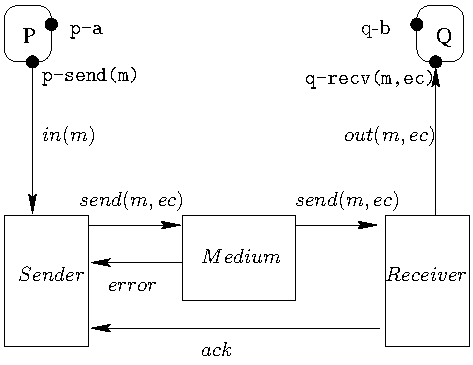
\includegraphics[width=5.5cm]{XFIG/SimpleProt-Schema}
%%    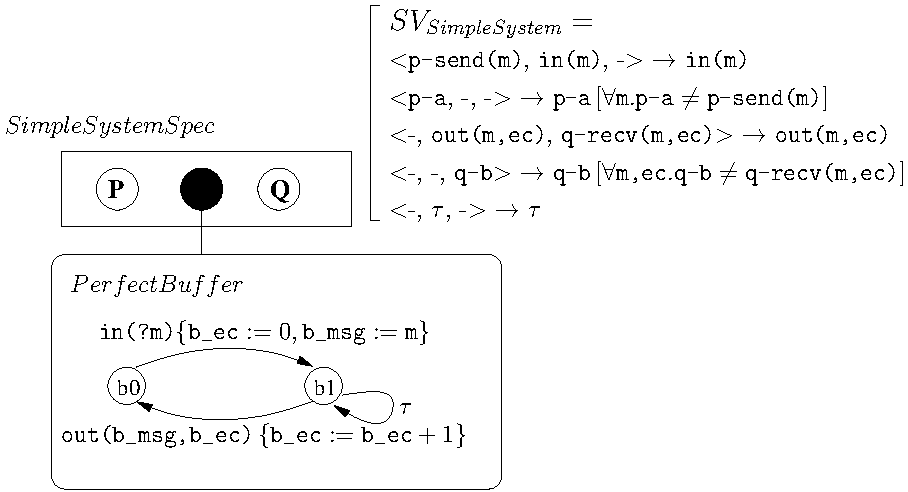
\includegraphics[width=6.5cm]{XFIG/SimpleProt2-Spec}
%%    \caption{Specification pNet Schema and Specification}
%%    \label{App:SimpleProt:Spec}

%% \end{figure}

  
%% \begin{figure}[t]
%%   \centerline{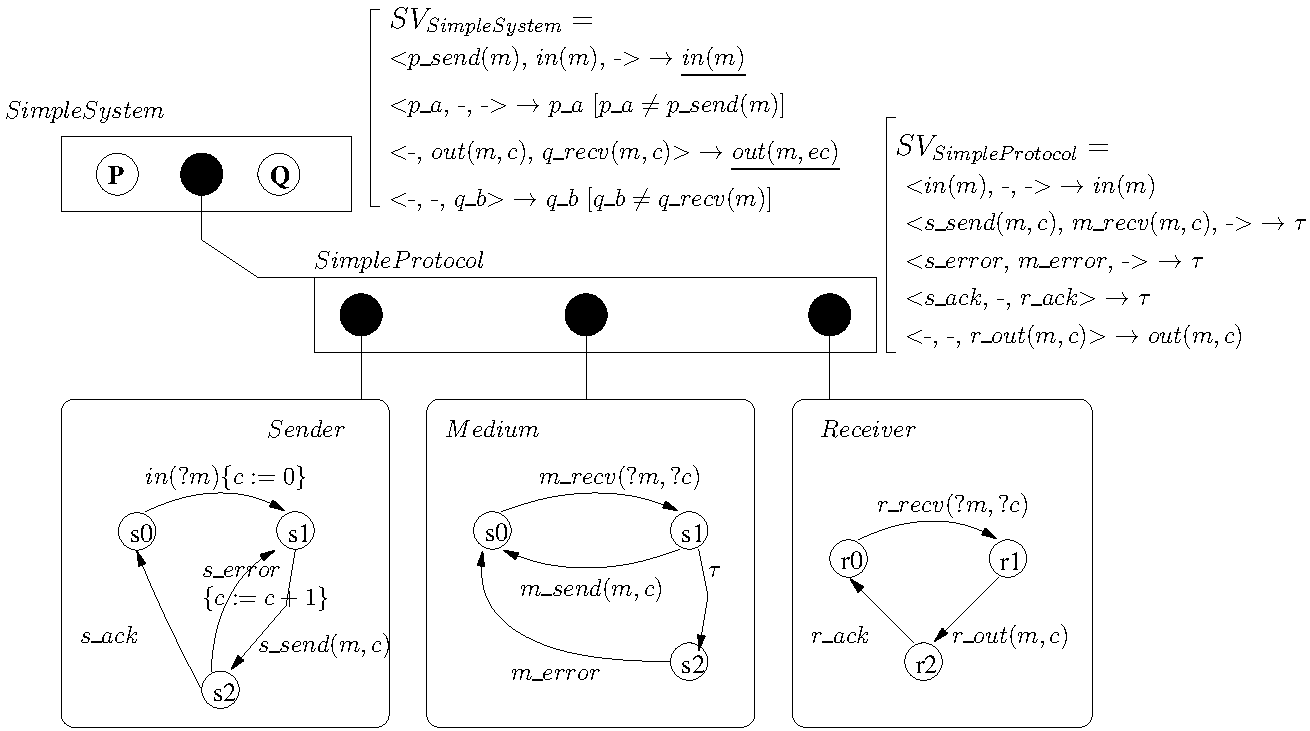
\includegraphics[width=12cm]{XFIG/SimpleProt2-pNet}}
%%   \caption{Composed pNet with the Simple Protocol Implementation}  \label{App:SimpleProt:Impl}
%% \end{figure}

The first piece of code is the textual definition of the SimpleProtSec
pNet, that was drawn in Figure \ref{SimpleProt:Impl}, page \pageref{SimpleProt:Impl}. This code should be intuitive enough to read, with the following
conventions, that brings some user-friendly features that are maps by the editor into pure pNet constructs.

\begin{itemize}
  \item Constants of any type (including Action) must be declared as
    ``const''. They are used either as functions with argument, as
    typically \texttt{in(msg)}, or constants without argument, denoted
    as \texttt{\$tau}. Identifiers without the ``?'' marker are
    variables.
  \item Variables can be declared either: inside a pLTS state (normal
    state variable), as global variable of a pLTS (see e.g. ...), or
    as an input variable in a transition, as \texttt{?msg} in pLTS M1
    here.
  \item the variables in the guards of synchronisation vectors do not need to be explicitely quantified: all variable in a guard that does not appear inside the vector actions will be recognised as bound by a \emph{foral} quantifier inside the guard.
    \item the tools will check that everything is correctly declared, and that variables are used properly, that vectors have coherent length, etc.
\end{itemize}

\TODO{Check coherency, the use-case figures have been modified}
%% \TODO{keep ?}
%% \paragraph{Variable management.}
%% The variables in each synchronisation vector are considered local:
%% for a given pNet expression, we must have fresh local variables for
%% each occurrence of a vector (i.e. each time we instantiate rule
%% \TrDeux). Similarly the state variables of each copy of a
%% given pLTS in the system, must be distinct, and those created for each
%% application of \TrDeux\ have to be fresh and all distinct. 
%% This is implemented within the open-automaton generation algorithm,
%% using name generation using a global counter as a suffix.

\begin{lstlisting}[basicstyle=\scriptsize\ttfamily, language=java, frame=single]
SimpleProtSpec2:
import "Data_Alg.algp"
root SimpleProtSpec2
const in, out:Action
const p_send, q_recv: Action
const tau:Action

pLTS M1
initial a0 
vars ?msg:Data

state a0
transition in(msg) -> a1 {a1_msg:=msg, m1_ec:=0}

state a1
vars a1_msg:Data m1_ec:Int
transition out(a1_msg, m1_ec) -> a0
transition synchro($tau)  -> a1 {m1_ec:=m1_ec+1}

pNet SimpleProtSpec2
holes P,Q
subnets P,M1,Q
vars p_a,q_a:Action m:Data ec:Int

vector SV0 <p_send(m), in(m),_>->synchro(in(m))
vector SV1 <p_a,_,_>->p_a [p_a != p_send(m)]
vector SV2 <_, out(m,ec), q_recv(m)>->synchro(out(m,ec))
vector SV3 <_,_,q_a>->q_a [q_a != q_recv(m)]

  \end{lstlisting}

The corresponding generated Open Automaton was given in Figure \ref{SimpleProtCounter:SpecOA},
page \pageref{SimpleProtCounter:SpecOA}.

Next is the code for the SimpleProtImpl pNet:

\begin{lstlisting}[basicstyle=\scriptsize\ttfamily, language=java, frame=single]
SimpleProtImpl2:
import "Data_Alg.algp"
root SimpleProtImpl2

const in,out:Action
const tau,p_send,q_recv,m_recv,m_send,m_error: Action
const s_recv,s_send,s_ack,s_error,r_recv,r_ack,r_send: Action

pLTS M1
  initial a0
  vars ?msg:Data ?c:Int

state a0
transition m_recv(msg,c) -> a1 {a1_msg:=msg, a1_ec:=c}

state a1
vars a1_msg:Data a1_ec:Int
transition m_send(a1_msg, a1_ec) -> a0 
transition synchro($tau) -> a2

state a2
transition $m_error -> a0

pLTS Sender
  initial s0
  vars ?msg:Data

state s0
transition s_recv(msg) -> s1 {s1_msg:=msg, s1_ec:=0}

state s1
vars s1_msg:Data s1_ec:Int
transition s_send(s1_msg, s1_ec) -> s2 {s2_ec:=s1_ec}

state s2
vars  s2_ec:Int
transition $s_ack -> s0
transition $s_error -> s1 {s1_ec:=s2_ec+1}

pLTS Receiver
  initial r0
  vars ?msg:Data ?c:Int

state r0
transition r_recv(msg,c) -> r1 {r1_msg:=msg, r1_ec:=c}

state r1
vars r1_msg:Data r1_ec:Int
transition r_send(r1_msg, r1_ec) -> r2

state r2
transition $r_ack -> r0

pNet medium
  subnets Sender, M1, Receiver
  vars m:Data c:Int
vector SV0 <s_recv(m), _, _>->in(m)
vector SV1 <s_send(m,c), m_recv(m,c), _>->synchro($tau)
vector SV2 <_, m_send(m,c), r_recv(m,c)>->synchro($tau)
vector SV3 <$s_ack, _, $r_ack>->synchro($tau)
vector SV4 <$s_error, $m_error, _>->synchro($tau)
vector SV5 <_, _, r_send(m,c)>->out(m,c)

pNet SimpleProtImpl2
  holes P,Q
  subnets P,medium,Q
  vars p_a,q_a:Action  m:Data c:Int
vector SV0 <p_send(m), in(m),_>->synchro(in(m))
vector SV1 <p_a,_,_>->p_a [p_a != p_send(m)]
vector SV2 <_, out(m,c), q_recv(m,c)>->synchro(out(m,c))
vector SV3 <_,_,q_a>->q_a [q_a != q_recv(m,c)]
\end{lstlisting}

%% From this code,A more compact view (maybe more readable ???) is given
%% by the pretty-printer of VerCors:

%% \begin{lstlisting}[basicstyle=\scriptsize\ttfamily, language=java, frame=single]
%% SimpleProtImpl2
%% --------------------
%% SV6 SVs: <p_send(m), in(m), _>-->in(m)
%% SV7 SVs: <p_a, _, _>-->p_a, p_a!=(p_send(m))
%% SV8 SVs: <_, out(m, c), q_recv(m, c)>-->out(m, c)
%% SV9 SVs: <_, _, q_a>-->q_a, q_a!=(q_recv(m, c))
%% SV11 SVs: <_, _tau_, _>-->_tau_
%% Holes: P
%% Subnets: medium
%% - medium
%% - SV0 SVs: <in(m), _, _>-->in(m)
%% - SV1 SVs: <s_send(m, c), m_recv(m, c), _>-->_tau_
%% - SV2 SVs: <_, m_send(m), r_recv(m)>-->_tau_
%% - SV3 SVs: <s_ack, _, r_ack>-->_tau_
%% - SV4 SVs: <s_error, m_error, _>-->_tau_
%% - SV5 SVs: <_, _, out(m, c)>-->out(m, c)
%% - SV10 SVs: <_, _tau_, _>-->_tau_
%% - pLTS: Sender
%% - - Transition: s0---in(msg)-->s1, { s1_msg := msg s1_ec := 0}
%% - - Transition: s1---s_send(s1_msg, s1_ec)-->s2, {}
%% - - Transition: s2---s_ack-->s0, {}
%% - - Transition: s2---s_error-->s1, { s1_ec := s2_ec+1}
%% - - Variable: s1_ec, State: s1, Value(s) = 0,s2_ec+1,
%% - - Variable: s1_msg, State: s1, Value(s) = msg,
%% - pLTS: M1
%% - - Transition: a0---m_recv(msg, c)-->a1, { a1_msg := msg a1_ec := c}
%% - - Transition: a1---m_send(a1_msg, a1_ec)-->a0, {}
%% - - Transition: a1---_tau_-->a2, {}
%% - - Transition: a2---m_error-->a0, {}
%% - - Variable: a1_msg, State: a1, Value(s) = msg,
%% - - Variable: a1_ec, State: a1, Value(s) = c,
%% - pLTS: Receiver
%% - - Transition: r0---r_recv(msg, c)-->r1, { r1_msg := msg r1_ec := c}
%% - - Transition: r1---out(r1_msg, r1_ec)-->r2, {}
%% - - Transition: r2---r_ack-->r0, {}
%% - - Variable: r1_msg, State: r1, Value(s) = msg,
%% - - Variable: r1_ec, State: r1, Value(s) = c,
%% Holes: Q
%% \end{lstlisting}

Finaly, we list here in raw format, the 19 OTs computed by the tool for the SimpleProtImpl pNet.
This view uses variable names very close to the internal representation in the tool, allowing for tracability of generated fresh variables. For example:
\begin{itemize}
\item m:SV6:1:1 refers to a variable named ``m'' in the synchronisation vector ``SV6''; the last 2 numbers allows to distinguish different clones.
\item the other variable names reflect our naming policy: state variables are prefixed by the name of the state, holes actions by the name of the hole.
\end{itemize}

\TODO{To be updated completely}

\begin{lstlisting}[basicstyle=\scriptsize\ttfamily, language=java, frame=single]

{P|->p_send(m:SV6:1:1)},
[(msg=m:SV0:12:1)/\((s_recv(msg))=(s_recv(m:SV0:12:1)))], {s1_msg := msg, s1_ec := 0}
	OT:1 ------------------------------------------------------------
		<s0_a0_r0>-----_in(m:SV6:1:1)_----><s1_a0_r0>

{P|->p_a:SV7:1:2},
[(forall:m:SV7:1:2. (p_a:SV7:1:2!=(p_send(m:SV7:1:2)))], {}
	OT:2 ------------------------------------------------------------
		<s0_a0_r0>-----p_a:SV7:1:2----><s0_a0_r0>

{Q|->q_a:SV9:1:4},
[(forall:m:SV9:1:4,c:SV9:1:4. (q_a:SV9:1:4!=(q_recv(m:SV9:1:4, c:SV9:1:4)))],   {}
	OT:3 ------------------------------------------------------------
		<s0_a0_r0>-----q_a:SV9:1:4----><s0_a0_r0>

INFO  SimpleProtImpl2 - 
{P|->p_a:SV7:1:2},
[(forall:m:SV7:1:2. (p_a:SV7:1:2!=(p_send(m:SV7:1:2)))],   {}
	OT:4 ------------------------------------------------------------
		<s1_a0_r0>-----p_a:SV7:1:2----><s1_a0_r0>

{Q|->q_a:SV9:1:4},
[(forall:m:SV9:1:4,c:SV9:1:4. (q_a:SV9:1:4!=(q_recv(m:SV9:1:4, c:SV9:1:4)))],   {}
	OT:5 ------------------------------------------------------------
		<s1_a0_r0>-----q_a:SV9:1:4----><s1_a0_r0>

{},   [(s1_msg=m:SV1:114:2)/\(s1_ec=c:SV1:114:2)
  /\((s_send(s1_msg, s1_ec))=(s_send(m:SV1:114:2, c:SV1:114:2)))
  /\(msg=m:SV1:114:2)/\(c=c:SV1:114:2)
  /\((m_recv(msg, c))=(m_recv(m:SV1:114:2, c:SV1:114:2)))],
{s2_ec := s1_ec, a1_msg := msg, a1_ec := c}
	OT:6 ------------------------------------------------------------
		<s1_a0_r0>-----_tau_----><s2_a1_r0>

{P|->p_a:SV7:1:2},
[(forall:m:SV7:1:2. (p_a:SV7:1:2!=(p_send(m:SV7:1:2)))],   {}
	OT:7 ------------------------------------------------------------
		<s2_a1_r0>-----p_a:SV7:1:2----><s2_a1_r0>

{Q|->q_a:SV9:1:4},
[(forall:m:SV9:1:4,c:SV9:1:4. (q_a:SV9:1:4!=(q_recv(m:SV9:1:4, c:SV9:1:4)))],   {}
	OT:8 ------------------------------------------------------------
		<s2_a1_r0>-----q_a:SV9:1:4----><s2_a1_r0>

{},   [(a1_msg=m:SV2:114:3)/\(a1_ec=c:SV2:114:3)
  /\((m_send(a1_msg, a1_ec))=(m_send(m:SV2:114:3, c:SV2:114:3)))
  /\(msg=m:SV2:114:3)/\(c=c:SV2:114:3)
  /\((r_recv(msg, c))=(r_recv(m:SV2:114:3, c:SV2:114:3)))],
{r1_msg := msg, r1_ec := c}
	OT:9 ------------------------------------------------------------
		<s2_a1_r0>-----_tau_----><s2_a0_r1>

		{},   [],   {}
	OT:10 ------------------------
		<s2_a1_r0>-----_tau_----><s2_a2_r0>

{P|->p_a:SV7:1:2},
[(forall:m:SV7:1:2. (p_a:SV7:1:2!=(p_send(m:SV7:1:2)))],   {}
	OT:11 ------------------------------------------------------------
		<s2_a0_r1>-----p_a:SV7:1:2----><s2_a0_r1>

{Q|->q_recv(m:SV8:1:3, c:SV8:1:3)},
[(r1_msg=m:SV5:18:6)/\(r1_ec=c:SV5:18:6)
  /\((r_send(r1_msg, r1_ec))=(r_send(m:SV5:18:6, c:SV5:18:6)))],   {}
	OT:12 ------------------------------------------------------------
		<s2_a0_r1>-----_out(m:SV8:1:3, c:SV8:1:3)_----><s2_a0_r2>

{Q|->q_a:SV9:1:4},
[(forall:m:SV9:1:4,c:SV9:1:4. (q_a:SV9:1:4!=(q_recv(m:SV9:1:4, c:SV9:1:4)))],   {}
	OT:13 ------------------------------------------------------------
		<s2_a0_r1>-----q_a:SV9:1:4----><s2_a0_r1>

{P|->p_a:SV7:1:2},
[(forall:m:SV7:1:2. (p_a:SV7:1:2!=(p_send(m:SV7:1:2)))],   {}
	OT:14 ------------------------------------------------------------
		<s2_a2_r0>-----p_a:SV7:1:2----><s2_a2_r0>

{Q|->q_a:SV9:1:4},
[(forall:m:SV9:1:4,c:SV9:1:4. (q_a:SV9:1:4!=(q_recv(m:SV9:1:4, c:SV9:1:4)))],   {}
	OT:15 ------------------------------------------------------------
		<s2_a2_r0>-----q_a:SV9:1:4----><s2_a2_r0>

		{},   [],   {s1_ec := s2_ec+1}
	OT:16 --------------------------------------
		<s2_a2_r0>-----_tau_----><s1_a0_r0>

{P|->p_a:SV7:1:2},
[(forall:m:SV7:1:2. (p_a:SV7:1:2!=(p_send(m:SV7:1:2)))],   {}
	OT:17 ------------------------------------------------------------
		<s2_a0_r2>-----p_a:SV7:1:2----><s2_a0_r2>

{Q|->q_a:SV9:1:4},
[(forall:m:SV9:1:4,c:SV9:1:4. (q_a:SV9:1:4!=(q_recv(m:SV9:1:4, c:SV9:1:4)))],   {}
	OT:18 ------------------------------------------------------------
		<s2_a0_r2>-----q_a:SV9:1:4----><s2_a0_r2>

		{},   [],   {}
	OT:19 ------------------------
		<s2_a0_r2>-----_tau_----><s0_a0_r0>


Assignements of state variables:

Global State: <s0_a0_r0>
===================
pLTS States: <s0 vars: {}> <a0 vars: {}> <r0 vars: {}>

Global State: <s1_a0_r0>
===================
pLTS States: <s1 vars: { s1_msg <-{msg} s1_ec <-{0, s2_ec+1}}> <a0 vars: {}> <r0 vars: {}>

Global State: <s2_a1_r0>
===================
pLTS States: <s2 vars: { s2_ec <-{s1_ec}}> <a1 vars: { a1_msg <-{msg} a1_ec <-{c}}> <r0 vars: {}>

Global State: <s2_a0_r1>
===================
pLTS States: <s2 vars: { s2_ec <-{s1_ec}}> <a0 vars: {}> <r1 vars: { r1_ec <-{c} r1_msg <-{msg}}>

Global State: <s2_a2_r0>
===================
pLTS States: <s2 vars: { s2_ec <-{s1_ec}}> <a2 vars: {}> <r0 vars: {}>

Global State: <s2_a0_r2>
===================
pLTS States: <s2 vars: { s2_ec <-{s1_ec}}> <a0 vars: {}> <r2 vars: {}>

INFO  SimpleProtImpl2 - Total: 19 SATISFIABLE OTs
INFO  SimpleProtImpl2 -        185 UNSATISFIABLE OTs
INFO  SimpleProtImpl2 - Total Time: 1105 ms

\end{lstlisting}

%% And here is a  drawing of this open automaton, slightly simplified for readability:

%% \begin{figure}[h]
%%   \centerline{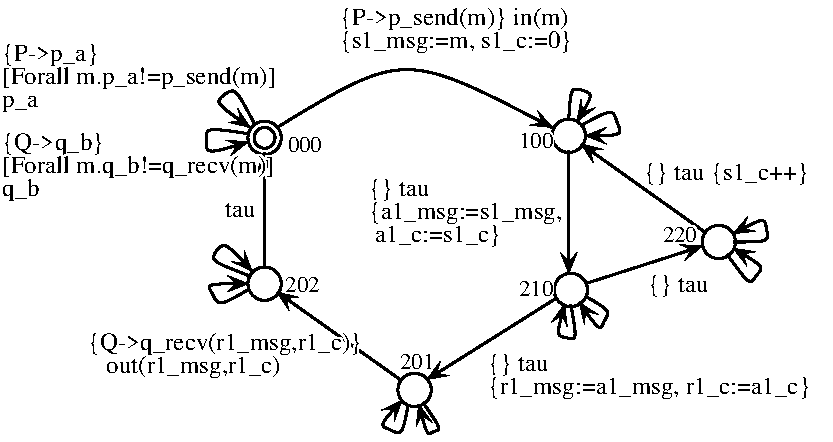
\includegraphics[width=10cm]{ATG/SPImplOpen}}
%%   \caption{Open Automaton of the Simple Protocol Implementation}  \label{Annex:SimpleProtCounter:ImplOA}
%% \end{figure}

%% And a partially saturated Automaton:

%% \begin{figure}[h]
%%   \centerline{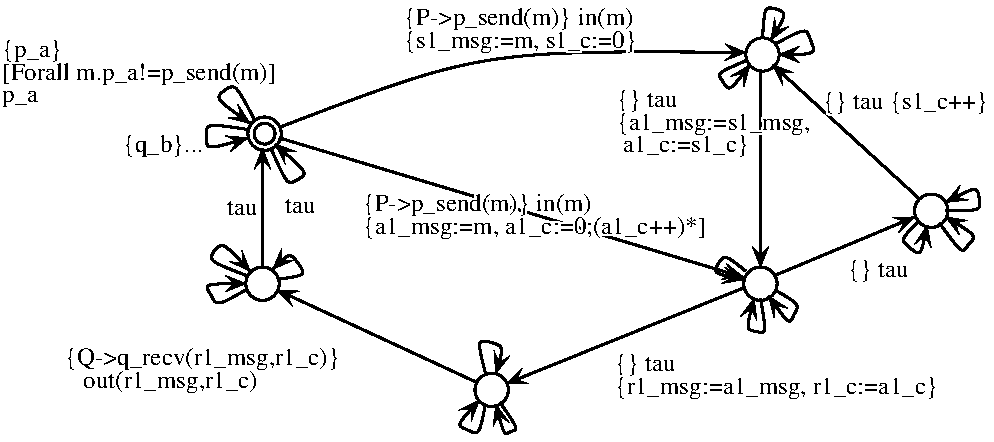
\includegraphics[width=13cm]{ATG/SPImplWeakOpen}}
%%   \caption{Weak Open Automaton, partial}  \label{SimpleProtCounter:ImplWOA}
%% \end{figure}

%% In Figure \ref{Annex:SimpleProtCounter:ImplWOA}, we have added some of the weak transitions generated by the saturation, namely:
%% - a tau-loop on each state
%% - a transition from <s0\_a0\_r0> to <s2\_a1\_r0>, resulting from the sequence OT\-1;OT\-6 followed by any number of the loop (OT\_9;ot\_12;OT\_6).
%%
%%Many weak should be added, e.g. Tau loops on states <s2\_a1\_r0>, <s2\_a2\_r0>, 
%%<s2\_a0\_r0>, encoding the loop.

\begin{figure}[h]
   \centerline{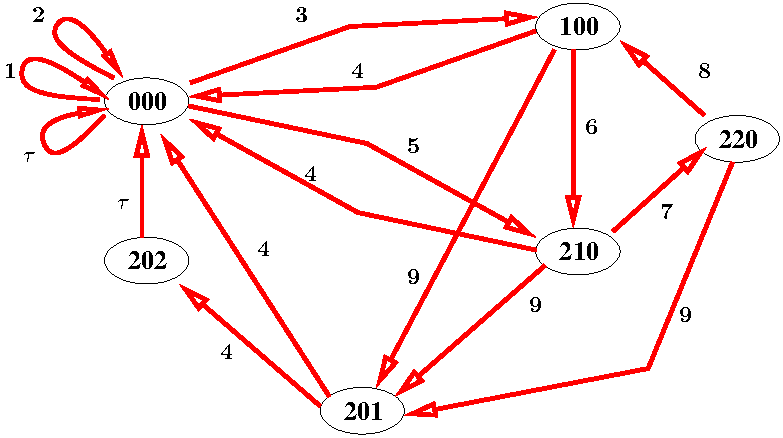
\includegraphics[width=9cm]{XFIG/SimpleProtImpl-WOA}}
  \caption{Weak Open Automaton of the implementation}
   \label{Appendix:SpecOA-partial}
\end{figure}

In Figure \ref{Appendix:SpecOA-partial} we show the weak open automaton of our implementation pNet. Details of the weak transitions is listed here:


$ WI_1 = \openrule
{\{\texttt{P}\mapsto \texttt{p-a}\}, [\forall \texttt{m}. \texttt{p-a} \neq \texttt{p-send(m)} ], ()}
{000 \OTWeakarrow {\tau} 000}$

$ WI_3(n) = \openrule
  {\{\texttt{P}\mapsto \texttt{p-send(m)}\}, True,
    (\texttt{s1\_msg}\gets \texttt{m}, \texttt{s1\_ec}\gets n)}
  {000 \OTWeakarrow {\underline{\texttt{in(m)}}} 100}
  \ \forall n\ge 0$

  $ WI_4(n) = \openrule
         {\{\}, True, (\texttt{m1\_msg}\gets \texttt{s1\_msg}, \texttt{m1\_ec}\gets \texttt{s1\_ec}+n, \texttt{s2\_ec}\gets \texttt{s1\_ec}+n)}
         {100 \OTWeakarrow {\tau} 210}
         \ \forall n\ge 0$

$Post_{8'''}= post_{8}\shortotimes\ post_{7}\shortotimes\ post_{4}\shortotimes\ Post_{456}^*\shortotimes\ post_{6} = (\texttt{r1\_msg}\gets \texttt{s1\_msg}, \texttt{r1\_ec}\gets \texttt{s2\_msg}+1+n), \forall n\ge 0$
         
$ WI_{8'''}(n) = \openrule
         {\{\texttt{Q}\mapsto \texttt{q-recv(s1\_msg,s2\_ec}+n)\}, True, ()}
         {210 \OTWeakarrow {\underline{\texttt{out(s1\_msg,s2\_ec+n)}}} 202}
         \ \forall n\ge 1$

\TODO{no yet checked...:}
         $ 1 = \openrule
{\{\texttt{P}\mapsto \texttt{p-a}\}, [\forall \texttt{m}. \texttt{p-a} \neq \texttt{p-send(m)} ], ()}
{000 \OTWeakarrow {\tau} 000}$

$ 2 = \openrule
{\{\texttt{Q}\mapsto \texttt{q-b}\}, [\forall \texttt{m}. \texttt{q-b} \neq \texttt{q-recv(m)} ], ()}
{000 \OTWeakarrow {\tau} 000}$


$ 5 = \openrule
         {\{\}, True, (\texttt{m2\_ec}\gets \texttt{m1\_ec}+n)}
         {210 \OTWeakarrow {\tau} 220}
         \ \forall n\ge 0$

$ 6 = \openrule
         {\{\}, True, (\texttt{s1\_ec}\gets \texttt{m2\_ec}+n)}
         {220 \OTWeakarrow {\tau} 100}
         \ \forall n\ge 0$

$ 7 = \openrule
         {\{\}, True, (\texttt{r1\_msg}\gets \texttt{s1\_msg}, \texttt{r1\_ec}\gets \texttt{s1\_ec}+n)}
         {100 \OTWeakarrow {\tau} 201}
         \ \forall n\ge 0$
         
$ 7' = \openrule
         {\{\}, True, (\texttt{r1\_msg}\gets \texttt{m1\_msg}, \texttt{r1\_ec}\gets \texttt{m1\_ec}+n)}
         {210 \OTWeakarrow {\tau} 201}
         \ \forall n\ge 0$
         
$ 7'' = \openrule
         {\{\}, True, (\texttt{r1\_msg}\gets \texttt{m1\_msg}, \texttt{r1\_ec}\gets \texttt{m2\_ec}+n)}
         {220 \OTWeakarrow {\tau} 201}
         \ \forall n\ge 1$
         
$ WI_8(n) = \openrule
         {\{\texttt{Q}\mapsto \texttt{q-recv(r1-msg,r1-ec +n)}\}, True, ()}
         {201 \OTWeakarrow {\underline{\texttt{out(r1-msg,r1-ec +n)}}} 202}
         \ \forall n\ge 0$

$ WI_9(n) = \openrule
         {\{\}, True, (\texttt{m1\_ec}\gets \texttt{m1\_ec}+n)}
         {210 \OTWeakarrow {\tau} 210}
         \ \forall n\ge 0$



         \subsection{Details of the Bisimulation Checking}
         \TODO{To be added}
         
\end{document}


%% \section{Examples of Lotos laws}
%% Possible Lotos small examples:

%% Strong bisim:\\
%% 1) Hiding:\\
%% \centerline{hide \{g\} in a;B  ==  a; hide \{g\} in B  iff gatename(a)$\neq$g}\\
%% \centerline{hide \{g\} in a;B  ==  i; hide \{g\} in B  iff gatename(a)$=$g}
%% 2) Disabling:\\
%% \centerline{B1[>(B2[>B3) == (B1[>B2)[>b3}\\
%% \centerline{(B1[>B2)[]B3 == B1[>B2}\\
%% \centerline{B[>stop == B}\\
%% \centerline{stop[>B == B}\\
%% \centerline{exit(...)[>B == exit(...)[]B}\\
%% 3) Enabling:\\
%% \centerline{B1>>(B2>>B3) == (B1>>B2)>>b3}\\
%% \centerline{B>>stop == B|||stop}\\
%% \centerline{stop>>B == stop}\\
%% \centerline{exit>>B == i;B}\\
%% 4) Choice:\\
%% \centerline{B1[](B2[]B3) == (B1[]B2)[]b3}\\
%% \centerline{B1[]B2 == B2[]B1}\\
%% \centerline{B[]stop == B}\\
%% \centerline{B[]B == B}\\

%% 5) Others:\\
%% \centerline{B1|[]|B2 == B1|||B2}\\


      
%% Weak congruence:\\
%% \centerline{a;i;B == a;B}\\
%% \centerline{B[]i;B == i;B}\\
%% and many others, often not easy to express without syntax for set operations,
%% like e.g.:
%% \centerline{}


%% Weak equivalence:\\
%% \centerline{i;B == B}

